\documentclass[a4paper, 12pt, oneside]{book}

\usepackage[utf8]{inputenc}
\usepackage{lmodern}
\usepackage{layout}
\usepackage{emptypage}
\usepackage{fancyhdr}
\usepackage[spanish,es-tabla]{babel}
%\usepackage[Conny]{fncychap}
%\usepackage{graphicx}
\usepackage{subfigure} % subfiguras
\usepackage{caption}
\usepackage{mathtools}
\usepackage{hyperref}
\usepackage[a4paper,top=3cm, bottom=3cm, inner=2.5cm, outer=2.5cm]{geometry}
\usepackage{listings}
\usepackage[spanish]{babel}
\usepackage{url}
\usepackage{float}
\usepackage{multirow}
\usepackage{rotating} 
\usepackage{color}
\usepackage{colortbl}
\usepackage[table]{xcolor}
\usepackage[spanish]{babel}
\usepackage{enumerate}
\usepackage{natbib}
\usepackage[acronym, nonumberlist]{glossaries}
\makeglossaries
\newacronym{hdf5}{HDF5}{Hierarchichal Data Format version 5}
\newacronym{ia}{IA}{Inteligencia Artificial}
\newacronym{ice}{ICE}{Internet Communications Engine}
\newacronym{rna}{RNA}{Redes Neuronales Artificiales}
\newacronym{va}{VA}{Visión Artificial}
\newacronym{xml}{XML}{Extensible Markup Language}
\newacronym{yolo}{YOLO}{You only look once}
\newacronym{coco}{COCO}{Common Objects in Context}
\newacronym{tfm}{TFM}{Trabajo de Fin de Máster}
\newacronym{cuda}{CUDA}{Compute Unified Device Architecture}
\newacronym{cntk}{CNTK}{The Microsoft Cognitive Toolkit}
\newacronym{opencv}{OpenCV}{Open Source Computer  Vision Library}
\newacronym{gmm}{GMM}{Gaussian mixture models}
\newacronym{mog}{MOG}{Mixture of Gaussian}
\newacronym{mei}{MEI}{Motion Energy Images}
\newacronym{em}{EM}{Expectation Maximization}
\newacronym{rcnn}{R-CNN}{Region-based Convolutional Neural Network}
\newacronym{cnn}{CNN}{Convolutional Neural Network}
\newacronym{svm}{SVM}{Support Vector Machine}
\newacronym{hog}{HOG}{Histogram of Oriented Gradients}
\newacronym{kaa}{KAA}{Kernel Auto Associator}
\newacronym{eoh}{EOH}{(Edge Orientation Histogram}
\newacronym{mbf}{MBF}{Measurement Based Features}
\newacronym{iphog}{IPHOG}{Intensity-based on a Pyramid of Histogram of Gradient Orientations}
\newacronym{sift}{SIFT}{Scale-Invariant Feature Transform}
\newacronym{klt}{KLT}{Kanade–Lucas–Tomasi }
\newacronym{sad}{SAD}{Sum of Absolute Differences}
\newacronym{gram}{GRAM-RTM}{GRAM Road-Traffic Monitoring}
\newacronym{ssd}{SSD}{Single Shot Detector}
\newacronym{nms}{NMS}{Non-Maximum Suppression} % Archivo que contiene los acrónimos

\makeatletter
\renewcommand{\@makeschapterhead}[1]{%
%  \vspace*{50\p@}%
  \vspace*{0\p@}%
  {\parindent \z@ \raggedright
    \normalfont
    \interlinepenalty\@M
    \Huge \bfseries  #1\par \nobreak
%    \vskip 40\p@
    \vskip 15\p@
  }}
\makeatother

\renewcommand{\baselinestretch}{1.4}
\setlength{\headheight}{16pt} 
\captionsetup{justification=justified}
\pretolerance=1000

\chead[]{}
\rhead[]{}
\renewcommand{\headrulewidth}{0.5pt}

\pagestyle{empty}

\title{Titulo}
\author{Jessica Fernández Martínez}

\lstset{
	float=hbp,
	basicstyle=\ttfamily\small,
	columns=flexible,
	tabsize=4,
	frame=single,
	extendedchars=true,
	showspaces=false,
	showstringspaces=false,
	numbers=none,
	numberstyle=\tiny,
	breaklines=false,
	breakautoindent=true,
	captionpos=b
}
\setcounter{tocdepth}{4}
\setcounter{secnumdepth}{4}

\definecolor{lightgray}{gray}{0.9}

\begin{document}
%%%%%%%%%%%%%%% Portada %%%%%%%%%%%%%%%%%%%%
\begin{titlepage}
	\begin{center}
		\vspace*{3mm}
		\begin{center}
			
\includegraphics[width=0.4\linewidth]{figures/logo.jpg}
		\end{center}
		\vspace{6.5mm}
		
		\fontsize{15.5}{14}\selectfont ESCUELA TÉCNICA SUPERIOR DE INGENIERÍA DE INFORMÁTICA
		\vspace{13mm}
		
		\fontsize{14}{14}\selectfont MÁSTER UNIVERSITARIO EN VISIÓN ARTIFICIAL 
		
		\vspace{55pt}
		
		\fontfamily{lmss}\fontsize{15.7}{14}\selectfont \textbf{TRABAJO FIN DE MÁSTER} 
		
		\vspace{20mm}
		\begin{huge}
			Monitorización Visual de Tráfico Rodado usando DeepLearning
		\end{huge}
		
		\vspace{20mm}
		
		\begin{large}
			Autor: Jessica Fernández Martínez
			
			Tutor: José María Cañas Plaza
			
			Co-tutor: Redouane Kachach
			
			
			\vspace{10mm}
		\end{large}
		\begin{normalsize}
			Curso académico 2018/2019		
		\end{normalsize}
		\vspace{10mm}
		
	\end{center}
	
\end{titlepage}

\pagenumbering{Roman}

%%%%%%%%%%%%%%% Agradecimientos %%%%%%%%%%%%
\chapter*{Agradecimientos}

Me  gustaría  dedicar  este  proyecto  a  toda  la  gente  que  me  ha  apoyado  durante  su realización. Sobre todo  a mis padres  y hermana que siempre están ahí y me ayudan en todo lo que necesito, pues sin ellos no hubiese sido posible conseguirlo.

Agradecer a mi familia todo el interés que han mostrado y como han conseguido que el trabajo fuera más sencillo.También quiero mencionar a mis amigos, los cuales siempre me han dado ánimos e incluso ideas para poder realizar el proyecto.

Por  último,  y  no  menos  importante,  quiero  agradecer  a  mi  tutor  José María todo el apoyo y sabiduría que me ha dado durante el proceso. Sin su dedicación y paciencia nada hubiera sido posible.


%%%%%%%%%%%%%%% Resumen %%%%%%%%%%%%%%%%%%%%
\chapter*{Resumen}

La gestión del tráfico es un tema muy complejo, pero com mucha importancia pues tiene grandes repercusiones. Esta gestión siempre se ha realizado de forma \textit{clásica}, mediante una cámara que se centraba únicamente en capturar imágenes y un operario era el encargado de extraer información de estas. En las últimas décadas se está tratando de automatizar todas aquellas cosas que pueden realizarse sin necesidad de que el ser humano actue tan activamente.

Las cámaras son el sensor principal en la gestión del tráfico, ya que son las que capturan las imágenes de donde se extraerá la información. Por tanto se puede decir que las imágenes son las que saben que está ocurriendo realmente en todo momento. Partiendo de esta premisa cada  vez se está tendiendo más a diseñar algoritmos capaces de extraer información de dichas imágenes, pues como se ha dicho son las principales fuentes de información. Por supesto, esto puede extenderse a la monitorización de vehículos.

El objetivo de este trabajo es crear un sistema capaz de extraer información de las imágenes con el objetivo de llegar a monitorizar una carretera mediante una única cámara. Este sistema se llama \textit{Smart-Traffic-Sensor} y parte de un sistema previo denominado \textit{Traffic-Sensor}~\cite{traffic_monitor_redo}, en el cual se llevaba a cabo la monitorización del tráfico haciendo uso de técnicas clásicas.

\textit{Smart-Traffic-Sensor} se centra en técnicas modernas como Deep Learning para la detección y clasificación de vehículos. La monitorización se fundamenta en criterios  de  proximidad  espacial  y \acrfull{klt}. Para poder realizar todo el proyecto ha sido necesario crear una base de datos con suficiente información y una serie de videos donde poder evaluarlo.

El sistema se ha evaluado con diversos videos en condiciones diferentes con el fin de saber como se comportaría ante posibles cambios o en condiciones en cuanto a calidad peores.





\cleardoublepage

%%%%%%%%%%%%%%% Índices %%%%%%%%%%%%%%%%%%%%
%\cleardoublepage
\renewcommand{\tablename}{Tabla}
%\renewcommand{\listtablename}{Índice de tablas}
%\tableofcontents

%\cleardoublepage % Í­ndice de figuras
%\addcontentsline{toc}{chapter}{\listfigurename}
%\listoffigures

%\cleardoublepage % Í­ndice de tablas
%\addcontentsline{toc}{chapter}{Índice de tablas}
%\listoftables 
\cleardoublepage
\tableofcontents % indice de contenidos

\cleardoublepage
\listoffigures % indice de figuras
\addcontentsline{toc}{chapter}{Índice de figuras} % para que aparezca en el indice de contenidos

\cleardoublepage
\listoftables % indice de tablas
\addcontentsline{toc}{chapter}{Índice de tablas} % para que aparezca en el indice de contenidos


%%%%%%%%%%%%%%% Acronimos %%%%%%%%%%%%%%%%%%%%

% Incluye el listado de acrónimos utilizados en el trabajo. 
\printglossary[type=\acronymtype,title={Acrónimos}]
% Añade el resto de acrónimos si así se desea. Si no elimina el comando siguiente
\glsaddallunused  
 
 
%%%%%%%%%%%%%%% Capí­tulos %%%%%%%%%%%%%%%%%%
\pagestyle{fancy}
\pagenumbering{arabic}
\setlength{\parindent}{6mm}

\lhead[]{CAPÍTULO \thechapter. INTRODUCCIÓN}
\chapter{Introducción}\label{cap.introduccion}

Debido al crecimiento en la población se ha visto incrementada la cantidad de vehículos que se encuentran en circulación. Este incremento en la densidad de vehículos ha afectado en el tráfico y en la contaminación. Por ello se han ido buscando formas de mejorar la seguridad vial y el rendimiento en las carreteras. En este punto es donde intervienen las nuevas tecnologías, las cuales son capaces de ofrecernos mucha información para poder mejorar el tráfico. Esta aplicación de sistemas avanzados de información y comunicación a las infraestructuras de transporte y a los vehículos para mejorar la seguridad vial, la eficiencia y el rendimiento de las carreteras se denomina Sistemas inteligentes de transporte (SIT). Este area está en continuo desarrollo y con ello se pretende dotar a los vehículos de inteligencia para aportarnos información con la cual mejorar nuestra seguridad y monitorizar las redes de transporte para detectar posibles incidencias y mejorar el tráfico.


\begin{figure}[H]
  \begin{center}
    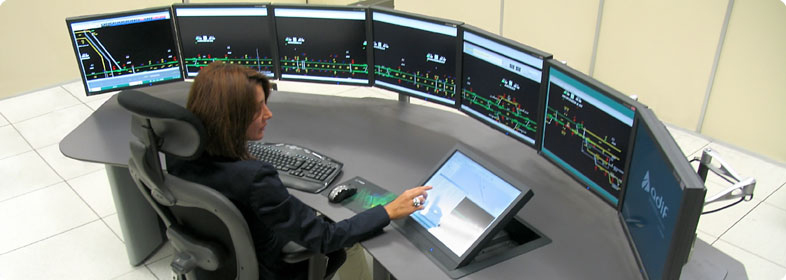
\includegraphics[width=0.6\textwidth]{figures/Introduccion/Indra.jpg}
		\caption{Centro de monitorización de tráfico}
		\label{fig.monitorizacion}
		\end{center}
\end{figure}

Los sistemas tradicionales de monitorización ofrecen una información muy limitada, pues normalmente es un humano el que analiza toda la información que le aportan las cámaras y con ello toma las decisiones. Gracias a los últimos avances en visión artificial muchas de las tareas que realizaba el humano se han podido automatizar. Con la visión artificial somos capaces de procesar todas las imágenes que recogen las cámaras y extraer información de ellas, como por ejemplo la cantidad de tráfico que hay, las condiciones meteorológicas que tenemos, la existencia de incidencias, etc.

Los principales sectores de los SIT son:
\begin{enumerate}
    \item Gestión avanzada del transporte
    \item Gestión avanzada del transporte público
    \item Sistemas de cobro automático
\end{enumerate}

El primer sector hace referencia a la gestión de carreteras a nivel global. Sus funciones principales son agilizar el tráfico, mejorar la movilidad, optimizar el uso de las infraestructuras y mejorar la seguridad de las redes de transporte. Para conseguir todo esto se emplea como sensor principal las cámaras. Con dichas cámaras se obtienen imágenes en todo momento, las cuales son procesadas y analizadas por seres humanos o automáticamente mediante algoritmos de visión artificial.  

El segundo sector tiene el mismo fin que el primer sector pero limitado a sistemas de transporte público. Entre sus funciones se encuentra gestionar de forma eficaz y optimizada las redes de transporte público, e informar  a los ciudadanos acerca de las distintas alternativas de transporte disponibles así como sus horarios o sus posibles incidencias en tiempo real. Este sector también se encarga de todo lo referente a los sistemas de cobro y el manejo de billetes en el transporte. Su objetivo es facilitar la integración y unificación de los sistemas de cobro para facilitar la creación de billetes multimodales y tarjetas de transporte subvencionadas por el estado.

El último sector (sector de cobro automático) se encarga de todos los sistema electrónicos de gestión de cuotas. La gestión de cobros automáticos en autopista con sistemas de telepeaje se basa en el empleo de sistemas inalámbricos de comunicación entre el sistema de gestión de cobro y el vehículo. En estos sistemas el vehículo debe disponer de un dispositivo, el cual permite identificarlos de manera segura y gestionar su cuota sin necesidad de que el vehículo se detenga en el telepeaje. Con esto se consigue reducir el atasco en los peajes.

A parte de la división a nivel sectorial de los SIT explicada, existe una división a nivel de aplicaciones. Esto puede verse en la Figura \ref{fig.division_SIT}.

\begin{figure}[H]
  \begin{center}
    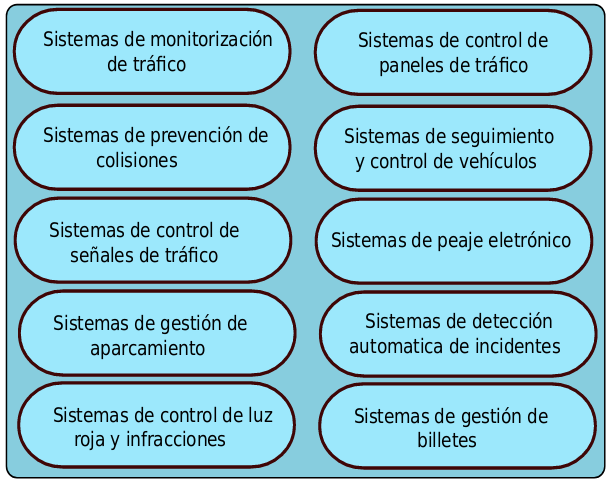
\includegraphics[width=0.6\textwidth]{figures/Introduccion/Division_SIT.png}
		\caption{División del sector SIT a nivel de aplicación}
		\label{fig.division_SIT}
		\end{center}
\end{figure}

\section{Cámaras en tecnologías automóviles y su entorno}

Si pensamos en una ciudad inteligente lo primero que nos viene a la cabeza son cámaras. Actualmente las cámaras se emplean en muchos ámbitos debido a la gran calidad que ofrecen, lo económicas que son y su reducido tamaño. Esto hace que sean uno de los mejores sensores de los que disponemos. Con las imágenes que nos ofrecen las cámaras necesitamos implementar algoritmos que sean capaces de procesarlas, extraer información y analizarla. Una de las aplicaciones pioneras donde la visión artificial ha demostrado ser una solución práctica frente a otras alternativas es la detección de matrículas. Este caso en concreto se usa en muchas puertas de acceso a aparcamientos, pues ha demostrado que tiene una gran fiabilidad. Además el hecho de encontrarse en puertas de acceso a aparcamientos hace que se trata de escenarios muy controlados, pues conocemos la iluminación del lugar, la posición que toman los vehículos, etc. Esto es una gran ventaja, pues nos aporta información adicional facilitándonos la identificación de las matrículas.

\begin{figure}[H]
  \begin{center}
    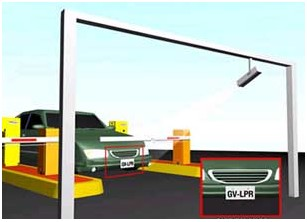
\includegraphics[width=0.6\textwidth]{figures/Introduccion/reconocimiento_matriculas.jpeg}
		\caption{Sistema de reconocimiento automático de matrículas}
		\label{fig.reconocimiento_matriculas}
		\end{center}
\end{figure}

Otra aplicación de las cámaras son los radares de tramo. En este caso se pretende calcular la velocidad media de cada vehículo haciendo uso del reconocimiento de matrículas. Las cámaras suelen situarse en los extremos de un túnel, ya que la trayectoria del vehículo está bajo control.

\begin{figure}[H]
  \begin{center}
    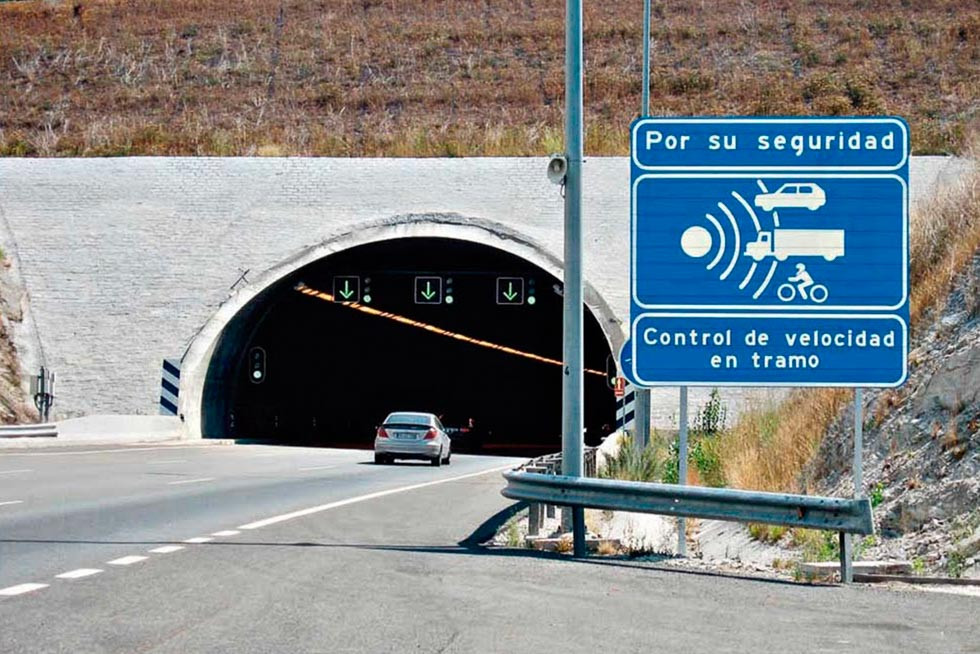
\includegraphics[width=0.6\textwidth]{figures/Introduccion/radartramo.jpg}
		\caption{Radar de tramo basado en reconocimiento de matrículas}
		\label{fig.radartramo}
		\end{center}
\end{figure}

Otro campo en el que cada vez tienen mayor relevancia las cámaras es en seguridad vial. Hoy en día hay varios modelos de coches capaces de detectar señales de tráfico de manera automática. De esta forma el vehículo puede avisar al conductor del exceso de velocidad, de la dirección de la próxima curva, etc. Este tipo de sistemas se encuentran incorporados en vehículos de marcas comerciales como BMW 7-series, Ford Focus, Toyota, Opel Insignia, etc.

\begin{figure}[H]
  \begin{center}
    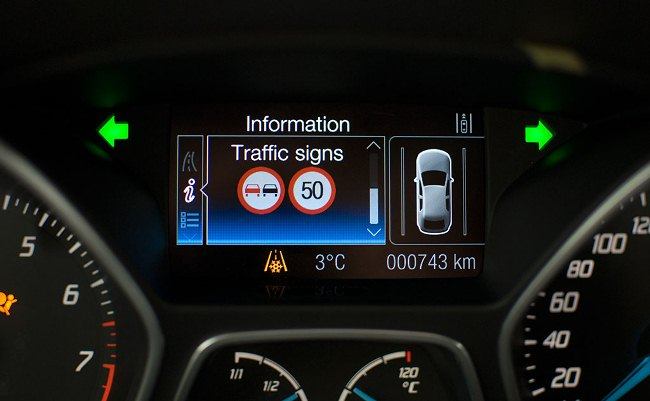
\includegraphics[width=0.6\textwidth]{figures/Introduccion/deteccion_senales.jpg}
		\caption{Sistema de ayuda a bordo del vehículo}
		\label{fig.deteccion_senales}
		\end{center}
\end{figure}

Disponer de cámaras en los vehículos ha hecho posible aumentar la seguridad, pues nos aportan mucha información. Actualmente existen modelos de vehículos que nos avisan de la presencia de peatones e incluso poseen mecanismos de frenado automático evitando posibles atropellos.

Una aplicación de las cámaras muy presente en los vehículos es el asistente para el aparcamiento.  En esta aplicación en concreto, las cámaras pueden aportar imágenes acerca de los alrededores de nuestro vehículo ,ofreciéndonos información acerca de como debemos aparcar, e incluso forman parte de  sistemas multisensoriales para aparcar automáticamente.

\begin{figure}[H]
  \begin{center}
    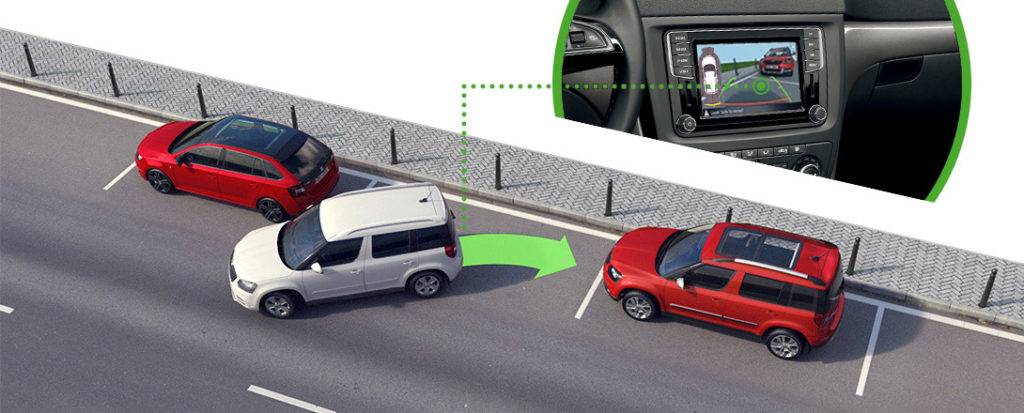
\includegraphics[width=0.6\textwidth]{figures/Introduccion/aparcamiento_automatico.jpg}
		\caption{Aparcamiento automático}
		\label{fig.aparcamiento_automatico}
		\end{center}
\end{figure}

Un ejemplo de asistencia en el aparcamiento es el sistema de ojo de pájaro de Nissan. Dicho sistema ofrece una vista aérea simulada de la escena del aparcamiento. En ella se incluye el vehículo y sus alrededores, ofreciéndole al conductor gran información acerca de la situación. Con lo que podrá realizar la maniobra de forma más sencilla y segura. Para conseguir esto, el vehículo dispone de 4 cámaras, las cuales emplea para generar la simulación. A parte de esta simulación, el conductor puede usar la cámara trasera para obtener más detalles de la escena.

\begin{figure}[H]
  \begin{center}
    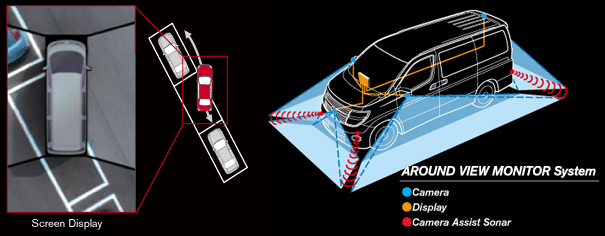
\includegraphics[width=0.6\textwidth]{figures/Introduccion/nissan.jpg}
		\caption{Sistema de visión de ojo de pájaro para asistencia en el aparcamiento}
		\label{fig.nissan}
		\end{center}
\end{figure}

BMW tiene un sistema un poco más evolucionado, pues  a parte del sistema de Nissan, posee una cámara trasera con sensores que miden las distancias con los obstáculos. En la imagen que ofrece proyecta una serie de líneas que ayudan en la orientación del vehículo durante la maniobra de aparcamiento. Estas imágenes son enriquecidas con marcas 3D que se basan en un código de color para marcar la distancia con los obstáculos. Además de todo esto, el sistema proporciona al conductor un mapa del vehículo y los obstáculos que le rodean en todo momento.

\begin{figure}[H]
  \begin{center}
    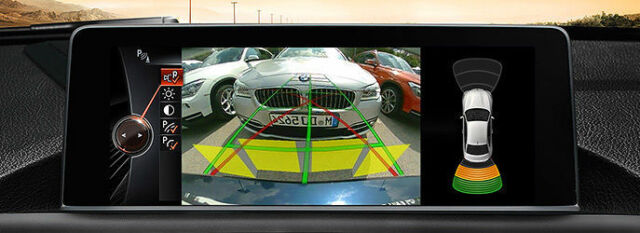
\includegraphics[width=0.6\textwidth]{figures/Introduccion/bmw.jpg}
		\caption{ Cámara trasera de BMW para asistencia en el aparcamiento}
		\label{fig.bmw}
		\end{center}
\end{figure}

Hoy en día uno de los campos en continua evolución es el de los coches autónomos, pues cada día hay más empresas interesadas en ello. Pero este tema no es tan actual, ya que en 1950 ya se trataba de crear coches autónomos. Y desde entonces se han conseguido continuos avances en su mayor medida destinados a aportar a los vehículos sistemas para navegar de forma autónoma.

Los coches autónomos disponen de un radar en la parte frontal para detectar vehículos próximos. Este sensor se emplea para mantener la distancia de seguridad con el vehículo que se encuentra delante y para posibles frenadas de emergencia si fueran necesarias. En las ruedas traseras tienen un sensor ultrasonido capaz de detectar obstáculos muy cercanos al vehículo, permitiendo con ello realizar maniobras muy precisas. Este sensor es muy práctico en el aparcamiento autónomo, pues ofrece información muy precisa en todo momento acerca de los obstáculos que se encuentren en la parte trasera. En la parte superior del vehículo se dispone de una antena GPS, una cámara Lidar y una cámara frontal. La antena GPS permite que el vehículo pueda localizarse con gran precisión en exteriores. La cámara Lidar (Light detection and ranging) realiza un barrido continuo de 360º para construir un mapa 3D de los alrededores del vehículo. La cámara frontal analiza todo lo que el vehículo tenga en frente, como por ejemplo señales de tráfico, peatones, otros vehículos, etc. A parte de todo lo comentado por supuesto contienen un ordenador a bordo que analiza la información captada por todos los sensores y en función a ella toma las decisiones que correspondan.Todos estos sensores pueden verse en la Figura \ref{fig.coche_autonomo}.

\begin{figure}[H]
  \begin{center}
    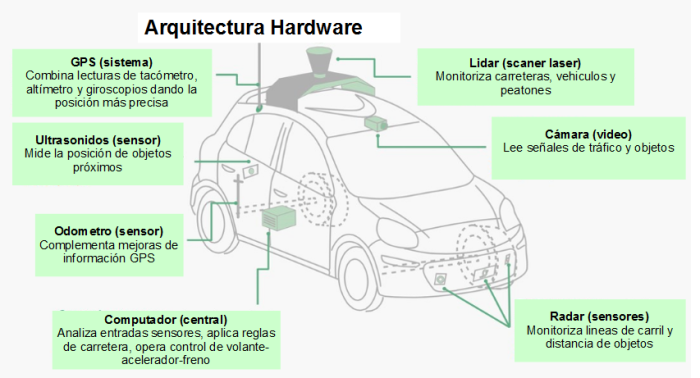
\includegraphics[width=0.6\textwidth]{figures/Introduccion/coche_autonomo.png}
		\caption{ Sensores en vehículos autónomos}
		\label{fig.coche_autonomo}
		\end{center}
\end{figure}

Si hablamos de conducción autónoma no nos podemos olvidar de mencionar al DARPA Grand Challenge. Se trata de una competición donde vehículos autónomos tratan de completar un circuito en el desierto en un tiempo determinado. En ella puede inscribirse cualquier entidad ya sea privada o pública. De hecho se pueden encontrar participando desde universidades hasta empresas privadas. Esta competición fue creada por la agencia de investigación DARPA con el objetivo de incentivar la creación y el desarrollo de vehículos autónomos capaces de  llevar a cabo misiones preplanificadas. Con ello se pretende poder emplear esta tecnología en misiones de exploración así como para aplicaciones militares.


La agencia DARPA también organiza la competición DARPA Urban Challenge. Esta competición tiene la misma dinámica que la mencionada anteriormente pero se desarrolla en un entorno urbano, el cual consta de 96km los cuales deben completarse en menos de 6 horas. Durante el trayecto los vehículos tienen que interactuar con otros vehículos autónomos o vehículos ocupados por conductores profesionales. En este caso la competición es más compleja que la comentada anteriormente, pues durante el circuito si tenemos señales de tráfico, las cuales deben respetarse. Con esto se pretende desarrollar vehículos que se puedan emplear en la vida cotidiana.

\begin{figure}[H]
  \begin{center}
    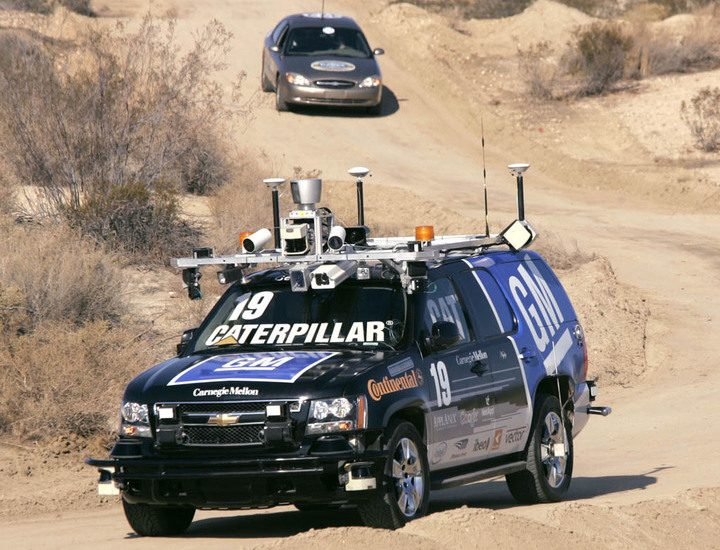
\includegraphics[width=0.6\textwidth]{figures/Introduccion/darpa.jpg}
		\caption{ Vehículo autónomo participante en el \textit{DARPA Grand Challenge}}
		\label{fig.darpa}
		\end{center}
\end{figure}


A pesar de todas las empresas implicadas en este desarrollo de vehículos autónomos la más famosa en este campo es Google. La división de coches autónomos de Google, conocida como Waymo, lleva varios años probando sus vehículos en situaciones reales. La única condición que tienen es que haya un conductor capaz de intervenir en caso de ser necesario ante una emergencia o posibles percances. Estos vehículos ofrecen continuamente información acerca de todo lo que les rodea, ya sea acerca de los peatones que hay, de los vehículos que les rodean, de las señales de tráfico, etc. Pues todo esto es por supuesto necesario para poder realizar una condución totalmente autónoma. El coche de Google además posee un sensor Lidar capaz de alcanzar una distancia máxima de 200 metros.

\begin{figure}[H]
  \begin{center}
    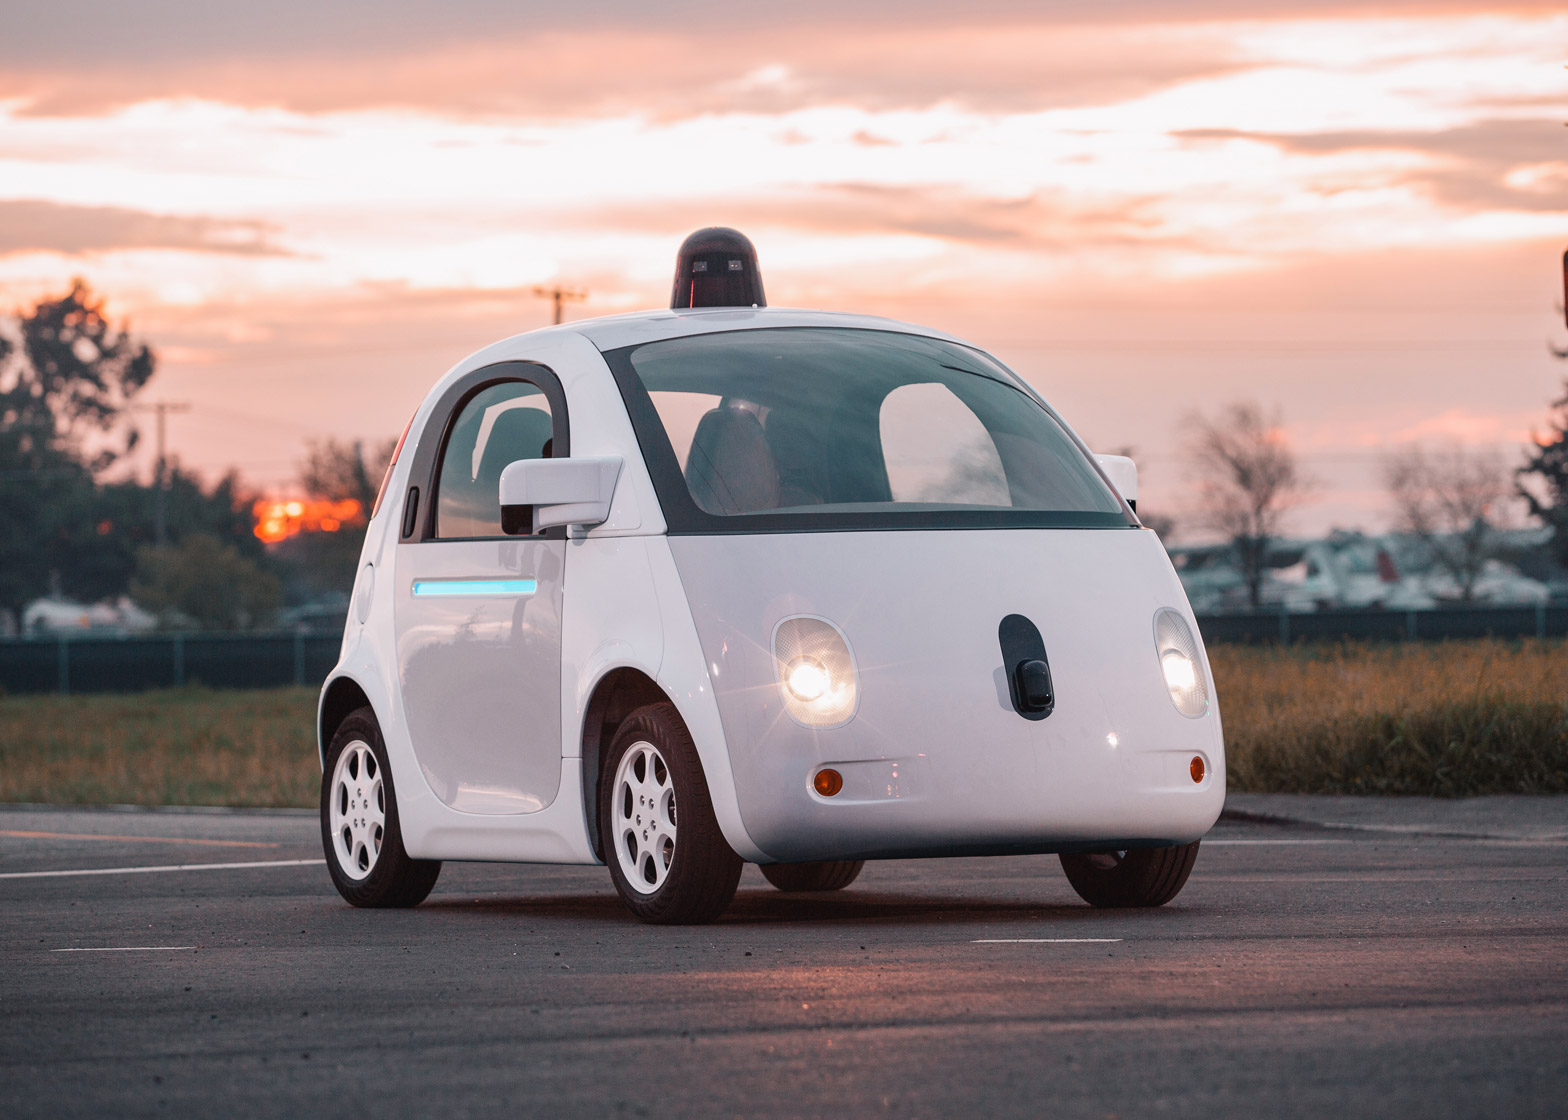
\includegraphics[width=0.6\textwidth]{figures/Introduccion/google_car.jpg}
		\caption{ Vehículo autónomo de Google}
		\label{fig.google_car}
		\end{center}
\end{figure}

Otra de las empresas más importantes en el desarrollo de vehículos autónomos es Tesla. Actualmente Tesla está comercializando el modelo S ,el modelo 3, el modelo X y el modelo Y, los cuales disponen de un piloto automático para activar la conducción autónoma, pero necesita una supervisión activa del conductor por si necesitará tomar el control en cualquier emergencia. A pesar de esto los nuevos vehículos Tesla tienen el hardware que será necesario en el futuro para una conducción completamente automática en la mayoría de situaciones. Pero la ley aún prohíbe dicha conducción autónoma sin supervisión del conductor. Además de esto poseen un asistente de aparcamiento, la posibilidad de aparcar automáticamente, un radar de largo alcance capaz de detectar peatones y obstáculos con una gran antelación, un sonar ultrasónico envolvente que monitoriza el coche desde todos los ángulos, cámaras que detectan señales de tráfico, peatones y otros vehículos, y un sistema de navegación GPS.

\begin{figure}[H]
  \begin{center}
    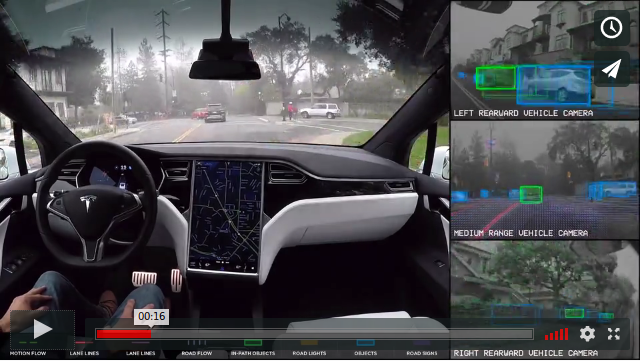
\includegraphics[width=0.6\textwidth]{figures/Introduccion/tesla.png}
		\caption{ Vehículo autónomo de Tesla}
		\label{fig.tesla}
		\end{center}
\end{figure}

\section{Las cámaras como sensor de tráfico}

En comparación con otras disciplinas, la aplicación de la visión computacional en el análisis del tráfico es un campo de estudio muy joven. Las primeras aplicaciones de este tipo fueron presentadas por Onoe  M.,  Ohba  K.~\cite{digital_analisis} y Hilbert~\cite{wide_area}. Pero hasta la década de los 80 no hubo una actividad constante de publicaciones. En este periodo ya podemos encontrar referencias a aplicaciones basadas en visión artificial y orientadas al análisis del tráfico de vehículos. Por ejemplo Hoose, N~\cite{queue_detection} en 1989 presentó una técnica para calcular de manera automática la longitud de la cola formada por vehículos parados o circulando a una velocidad muy reducida. Ese año J.M Blosseville, C. Krafft, F. Lenior,V. Motyka, S. Beucher~\cite{traffic_measurement} presentaron el sistema TITAN, el cual es capaz de analizar escenas de entre 100 hasta 300 metros de longitud, día y noche. Con ello extrae parámetros tales como el flujo de vehículos, la velocidad y la longitud de la cola en atascos, todo esto con una velocidad de procesamiento de 4 imágenes por segundo. Las características más importantes de este trabajo son las luces de noche y los techos, capós y sombras frontales de día. 

En 1989 Versavel, J. ;Lemaire, F. ; Van der Stede, D.~\cite{computer_aided} también presentó el sistema CCATS, el cual obtiene parámetros del tráfico como la ocupación de los carriles, el número de vehículos y la velocidad media de estos.

Además puede detectar anomalías en el flujo de vehículos como atascos o largas colas y alertar acerca de ello. Para mejorar el tráfico este sistema fue instalado en Bélgica.

Hasta finales de los 80 los trabajos se centraron en un macro análisis del tráfico para extraer datos relativamente simples. A partir de los 90 esto va a cambiar pues aumentará la investigación en este sector y se empezarán a realizar análisis más detallados de las escenas basándose en las características visuales de los vehículos. Es entonces cuando se empieza a usar plantillas 3D para la clasificación y seguimiento de vehículos. Baker, K.D Sullivan, G.D.~\cite{performance_assessment} se dedicaron a analizar la viabilidad del seguimiento del tráfico basándose en modelos 3D. Para este seguimiento de tráfico han empleado reconocimiento y estimación de posición en secuencias de imágenes. En esa época el reconocimiento y estimación de posición estaba pensado para una sola imagen , por lo que fueron pioneros al aplicarlo en secuencias de imágenes. En su trabajo disponían de información a priori acerca de la escena 3D, la cual obtenían mediante una cámara calibrada. A pesar de no funcionar en tiempo real este trabajo fue el que abrió las puertas hacia nuevos estudios relacionados con el seguimiento de vehículos.

Koller, D., Weber, J., Malik, J.~\cite{robust_multiple} presentaron un trabajo en el cual describían un sistema basado en el seguimiento de vehículos haciendo especial importancia en las oclusiones, uno de los grandes problemas en los sistemas de análisis de tráfico. En la Figura ~\ref{fig.koller_weber_walik_oclusion} podemos ver un ejemplo de su trabajo.

\begin{figure}[H]
  \begin{center}
    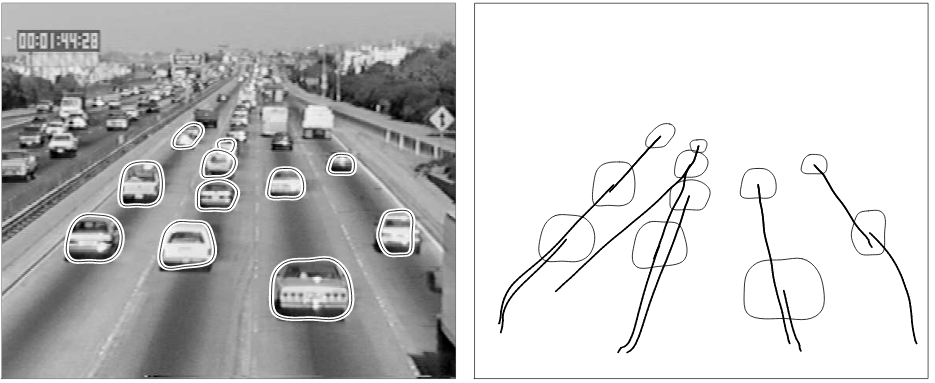
\includegraphics[width=0.9\textwidth]{figures/Introduccion/koller_weber_walik_oclusion.png}
		\caption{Ejemplo de detección y seguimiento de vehículos de~\cite{robust_multiple}}
		\label{fig.koller_weber_walik_oclusion}
		\end{center}
\end{figure}

G.D. Sullivan, K.D. Baker, A.D. Worral, C.I. Attwood, P.M. Remagnino~\cite{model_vehicle_detection} publicaron un sistema para la clasificación de vehículos empleando una combinación de plantillas en 1-D  y 2-D. Las plantillas 1-D se generaban sobre modelos de vehículos y las 2-D se empleaban para la verificación y aceptación de las hipótesis generadas en la primera fase del algoritmo de clasificación.Coifman et al.~\cite{areal_time} presentaron un algoritmo capaz de seguir un conjunto de características visuales de los vehículos ( en lugar del vehículo completo) con lo cual pretende ser más robusto ante oclusiones.

Las técnicas que se han ido publicando en las últimas décadas se presentan en dos escenarios (tráfico urbano y tráfico en autopistas). A continuación se explicará las situaciones que se encuentran en ambos escenarios.

\subsection{Visión computacional en tráfico urbano}\label{ap.vision_computacion_urbano}

En el análisis de tráfico urbano se pretende aplicar las técnicas de visión computacional en ciudades o entornos urbanos en general. En este caso la visión computacional se emplea para asegurar la aplicación de las normas de tráfico, para obtener información acerca del flujo de tráfico o para detectar posibles incidencias. El entorno urbano es un entorno muy complejo, pues existen demasiadas variables involucradas. Podemos tener peatones, ciclistas, edificios, señales de tráfico, árboles, otros vehículos, etc. Esto hace que sea más probable tener oclusiones en la imagen.

Una aplicación muy habitual en entornos urbanos es la detección de conductores que no respetan los semáforos en rojo. Para ello se   hace uso de cámaras que se encuentran conectadas a las luces del semáforo, y cada vez que éste se pone en rojo las cámaras se activan. Todo vehículo que sobrepasa la línea blanca una vez este el semáforo en rojo quedará fotografiado. Pero esto no siempre se tiene totalmente en cuenta, pues en muchas legislaciones es necesaria una prueba irrefutable de que el vehículo se ha saltado el semáforo. Esto se debe a que en muchos casos cuando un semáforo está en ambar los coches aceleran, corriendo el riesgo de pasar justo cuando el semáforo se ponga en rojo. Con el fin de evitar estos problemas, los sistemas han ido avanzando. Actualmente se graban toda la escena para poder asegurarse de si existe una infracción o no. La cámara se sitúa antes del semáforo para poder ver claramente a los vehículos infractores. Además se les ha incorporado un mecanismo para medir la velocidad de los vehículos que pasan y así poder ver si tienen alta probabilidad de saltarse los semáforos. Si superan cierta velocidad se considera que tienen una alta probabilidad de cometer una infracción y es entonces cuando la cámara se activa para grabarlo.
\begin{figure}[H]
  \begin{center}
    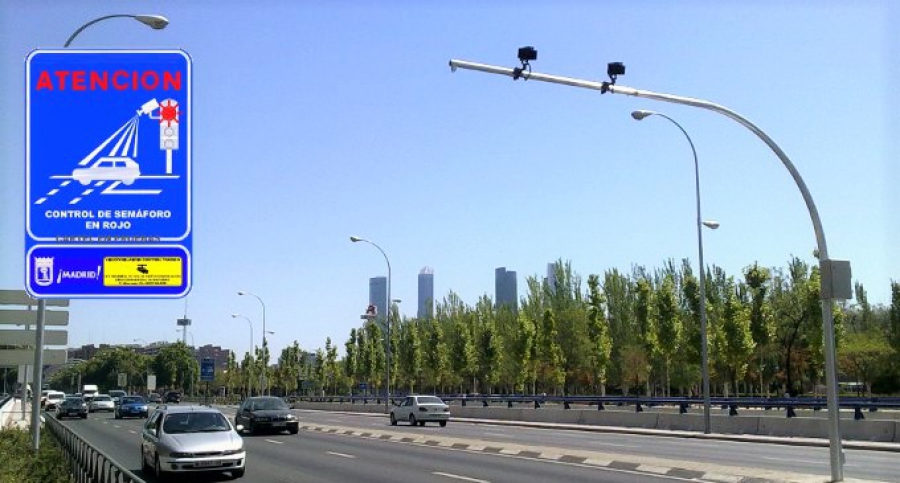
\includegraphics[width=0.6\textwidth]{figures/Introduccion/control_semaforo.jpg}
		\caption{Control de semáforos en rojo}
		\label{fig.control_semaforos}
		\end{center}
\end{figure}
En el tráfico interurbano una aplicación muy común es la detección de infracciones. Los centros de monitorización del tráfico disponen de muchas cámaras en las carreteras, pero el personal dedicado a revisar las imágenes que obtienen es bastante reducido, por lo que surge la necesidad de automatizar este proceso. A esta automatización de la detección de incidencias se le llama AID  y gracias a ella los trabajadores dedicados  a la monitorización del tráfico solo tienen que revisar las imágenes en las  cuales las cámaras han detectado una incidencia. El hecho de automatizar este proceso hace que el tiempo de intervención se vea reducido, pues son capaces de detectar las incidencias en menor tiempo, minimizando el tiempo de respuesta de los servicios sanitarios. Con esta información pueden actualizarse los paneles informativos, para avisar al resto de vehículos de la existencia de un accidente.

\begin{figure}[H]
  \begin{center}
    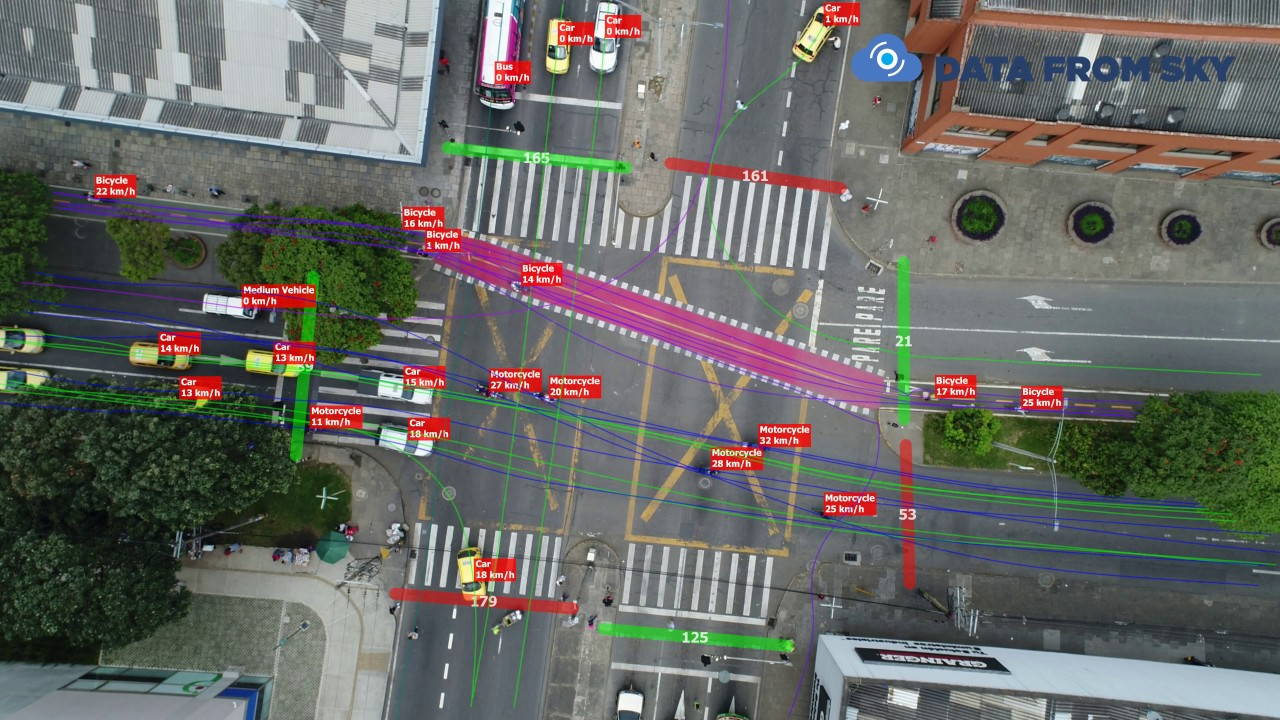
\includegraphics[width=0.75\textwidth]{figures/Introduccion/monitorizacion_trafico_urbano.jpg}
		\caption{Monitorización del tráfico urbano}
		\label{fig.monitorizacion_trafico_urbano}
		\end{center}
\end{figure}

Vermeulen~\cite{automatic_incident} para detectar incidentes combina la información visual con información obtenida por una cámara térmica. Con esto se consigue un sistema muy robustos ante las diferentes condiciones meteorológicas. Este sistema fue instalado en el puente de \textit{Rion} en Grecia. Chang et al~\cite{new_traffic_incident} presentó un sistema basado en la detección de matrículas para la identificación de incidencias. En este caso emplea la información del tiempo de viaje del vehículo para inferir incidencias en su trayectoria.

Otro tema en creciente desarrollo es el análisis del comportamiento de los vehículos en rotondas o bifurcaciones. A la hora de realizar modificaciones en las infraestructuras viales se realizan estudios acerca del flujo de vehículos que circulan por las redes de transporte, para ello es muy útil conocer el comportamiento de los vehículos. Nateghinia and Moradi~\cite{video_based_multiple} realizó un sistema capaz de seguir los vehículos en intersecciones y resolver el problema de las oclusiones. Para realizar las detecciones modelan cada píxel como una distribución gaussiana y lo combinan con el modelado dinámico de  textura. Shirazi and Morris~\cite{vision_based_turning} presentó un sistema un poco más evolucionado, pues a parte de seguir y contar los vehículos en cada intersección, era capaz de estimar la capacidad y el tiempo de espera en la intersección y reconstruir la trayectoria de los vehículos.

Finalmente, no hay que olvidarse de los túneles, los cuales juegan un papel importante dentro del tráfico urbano. De hecho en la M-30 en Madrid tenemos una longitud de 43 km de túneles, con el fin de reducir el flujo de tráfico sobre la superficie. Debido al gran uso de los túneles y la dificultad que existe para acceder a ellos en caso de accidentes, es necesario monitorizarlos. El uso de cámaras en los túneles hace que se pueda identificar la existencia de incidencias dentro de ellos, para actuar en el menor tiempo posible. En este caso una actuación rápida es esencial para evitar segundos accidentes o catástrofes en caso de incendios.

\begin{figure}[H]
  \begin{center}
    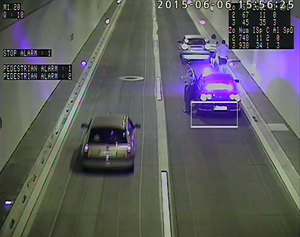
\includegraphics[width=0.6\textwidth]{figures/Introduccion/detection_tunel.png}
		\caption{Sistema de detección de incidencias en túnel}
		\label{fig.deteccion_tunel}
		\end{center}
\end{figure}

\subsection{Monitorización de autopistas basada en visión}

En este caso el análisis del tráfico se realiza en autopistas. Con ello se pretende obtener información acerca de la velocidad de los vehículos, el flujo de tráfico, la existencia de incidencias, etc. Este entorno es más sencillo que el comentado en el Apartado ~\ref{ap.vision_computacion_urbano}, ya que no hay que controlar tantas variables (peatones, edificios , etc), únicamente tendremos vehículos de diferentes tipos. 

\begin{figure}[H]
  \begin{center}
    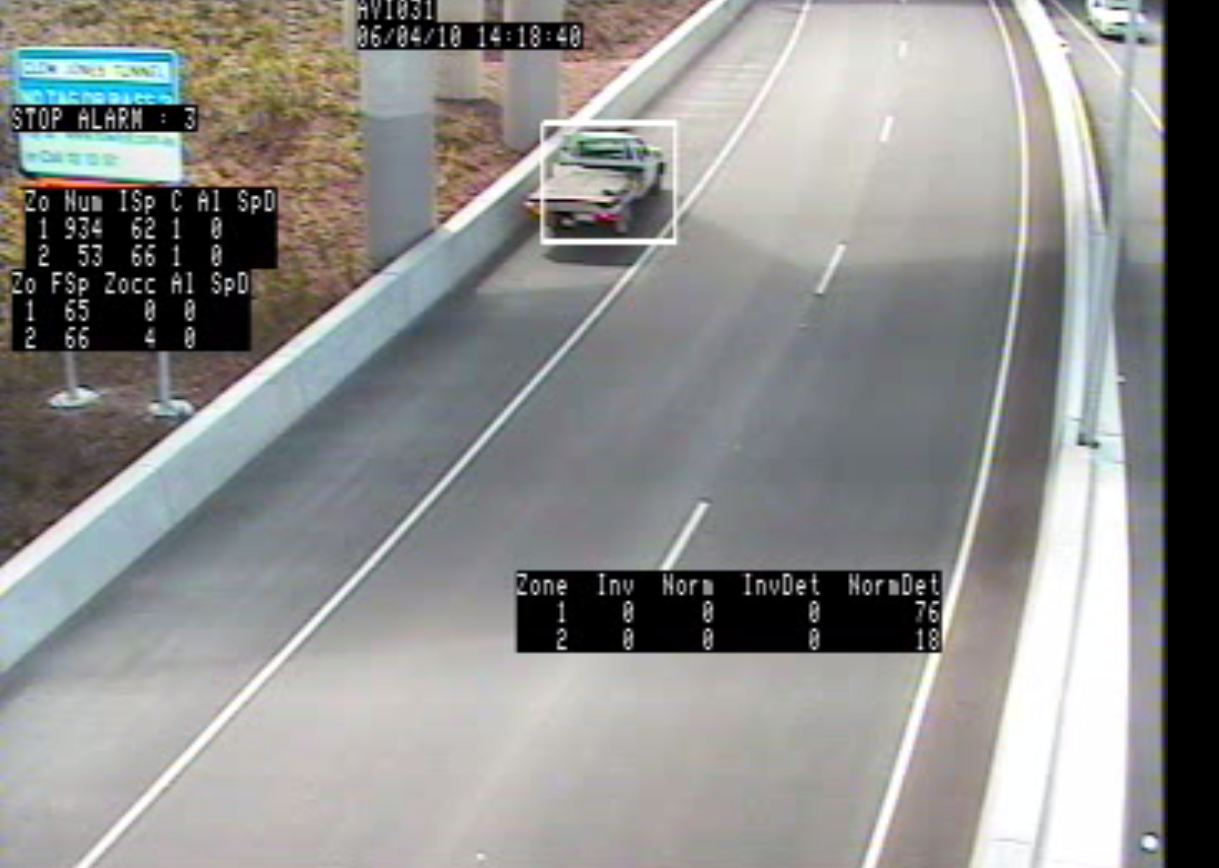
\includegraphics[width=0.6\textwidth]{figures/Introduccion/deteccion_autopistas.jpg}
		\caption{Sistema de detección de incidencias en autopistas}
		\label{fig.deteccion_autopistas}
		\end{center}
\end{figure}

La mayoría de los sistemas mencionados en el caso de entornos urbanos se emplean en las autopistas, ya que las incidencias que ocurren son similares. La principal diferencia entre ambos escenarios es la velocidad de los vehículos. En el tráfico urbano el límite de velocidad es bajo, pero en las autopistas es mucho más elevado y depende de cada país. En España el límite esta en 120km/h pero en Alemania la velocidad no está limitada. Esto se debe tener en cuenta a la hora de realizar el sistema de monitorización.

\section{Sistemas comerciales basados en visión}

Antiguamente la visión computacional solo se desarrollaba en el ámbito de la investigación pero actualmente se ha visto extendida hasta un ámbito comercial. Actualmente en el mercado hay numerosos sistemas basados en visión. Gracias a su reducido coste y su gran fiabilidad los sistemas basados en visión se han convertido en una alternativa perfecta a los sistemas clásicos de detección.

Desde los años 80 el empleo de la tecnología en los sistemas inteligentes de transporte ha ido creciendo. Esto se debe a que es un sector muy importante en los países en vías de desarrollo y en los países desarrollados. Algunas de las empresas que desarrollan este tipo de sistemas son: Flir (EEUU), Siemens (Alemania), Indra (España), Kapsch (Austria), Q-Free (Norguega), Thales (Francia), Sigtec(Austria).

Siemens es uno de los mayores proveedores de sistemas de control de tráfico a nivel mundial. Su familia de sistemas \textit{SitTraffic} ofrece un amplio abanico de funcionalidades.

FLIR es una empresa muy activa en este sector, pues ofrece sistemas con diversas funciones (detección automática de atascos, presencia de vehículos en las intersecciones, detección de peatones , etc).  Su sistema combina cámaras visuales y cámaras térmicas que le permiten regular las luces de tráfico. La serie de productos \textit{TrafiCam} realiza la detección y seguimiento de vehículos en intersecciones de forma automática; y permite posicionar y verificar con exactitud las zonas de detección de presencia de vehículos. Además este sistema mide la longitud de las colas que se forman en los atascos.

\begin{figure}[H]
  \begin{center}
    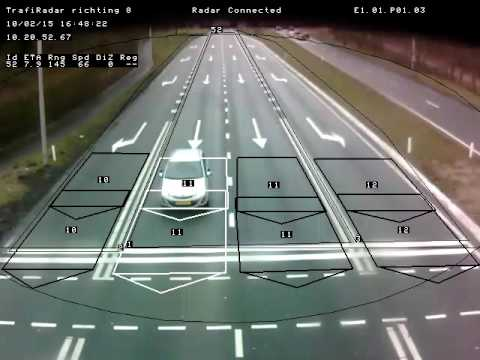
\includegraphics[width=0.6\textwidth]{figures/Introduccion/flir.jpg}
		\caption{Sistema \textit{TraffiCam} de FLIR}
		\label{fig.flir}
		\end{center}
\end{figure}

La empresa Morpho ha desarrollado un sistema basado en visión que pretende sustituir a los radares tradicionales. Se trata de su sistema \textit{Mesta Fusion}, el cual es capaz de detectar coches que circulen hasta a 300 km/h, puede controlar ocho carriles al mismo tiempo, supervisar 32 vehículos a la vez y discriminar entre ellos según sea un turismo, una moto, una furgoneta o un camión o autobús. Además es capaz de identificar casi cualquier acción indebida.  Todo eso lo hace un sistema perfecto en temas de monitorización de tráfico. Este sistema ya está operativo en Francia y Dubai.

\begin{figure}[H]
  \begin{center}
    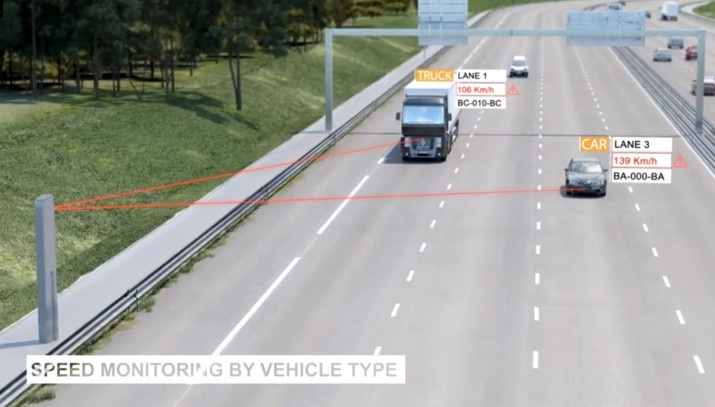
\includegraphics[width=0.6\textwidth]{figures/Introduccion/mesta_fusion.jpg}
		\caption{Sistema \textit{Mesta Fusion} de Morpho}
		\label{fig.mesta_fusion}
		\end{center}
\end{figure}

\section{Redes Neuronales}

Las \acrfull{rna} son un modelo matemático que pretende asemejarse al comportamiento biológico de las neuronas. Su objetivo principal es poder aprender al igual que lo hacen los seres humanos, para ello siguen una estructura jerárquica similar.

Las neuronas biológicas poseen un cuerpo celular que contiene un núcleo, una serie de ramas denominadas dendritas y un axón. Las dendritas transmiten la información de las células vecinas mediante sinapsis al cuerpo celular, y éste genera impulsos nerviosos para transmitir la información a otras neuronas a través del axón.

En las redes neuronales la sinapsis y las dendritas son las entradas, y el proceso interno es el cuerpo neuronal. Cada entrada tiene asociado un peso. Estos pesos se multiplican por las propias entradas. Normalmente se suma el resultados de estos productos y se genera un resultados que se transmite por la salida o axón. En la Figura ~\ref{fig.neurona} se puede ver una comparativa de las neuronas biológicas y las artificales.

\begin{figure}[H]
  \begin{center}
    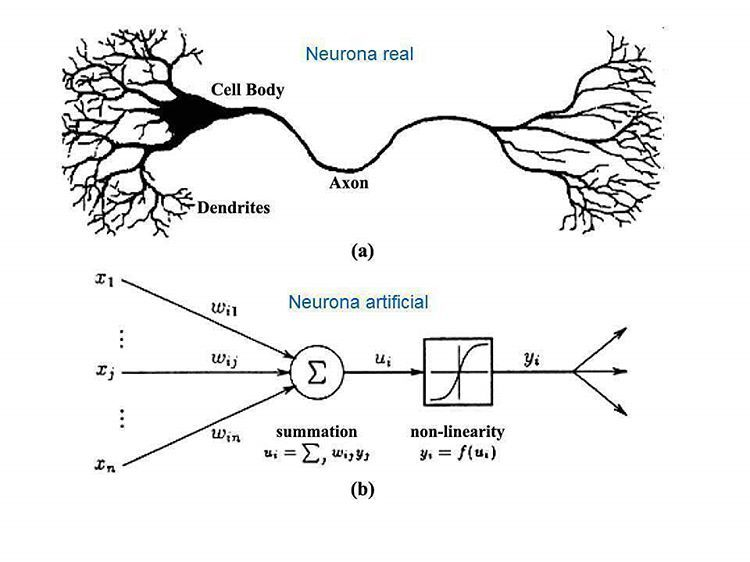
\includegraphics[width=0.7\textwidth]{figures/Introduccion/neurona.jpg}
		\caption{Neurona Biológica y Artificial}
		\label{fig.neurona}
		\end{center}
\end{figure}

Actualmente las \acrshort{rna} han tomado mucha relevancia en el mundo de la \acrfull{va} debido a sus grandes resultados. Pues se ha visto que son capaces de aprender gran cantidad de características.


\section{Objetivos}

Este \acrfull{tfm} se basa en la monitorización visual de vehículos mediante el uso de una cámara. El objetivo principal de este proyecto es obtener un sistema capaz de detectar, clasificar y realizar un seguimiento de vehículos en tiempo real. Para ello se ha partido de un sistema inicial realizado por Redouane Kachach~\cite{redo_tesis}(\textit{Traffic-Monitor~\cite{traffic_monitor_redo}} en su tesis doctoral. Dicho sistema se basa en técnicas clásicas. El objetivo es mejorar sus resultados con el uso de técnicas más actuales como el \textit{Deep Learning}.

La detección se basa en identificar la posisición de los vehículos en la imagen. Al hacer uso de \textit{Deep Learning} la detección y clasificación de vehículos van de la mano. En este trabajo se evaluaran diferentes  librerías relacionadas con el \textit{Deep Learning}, tales como \textit{TensorFlow}, \textit{Keras} y \textit{Darknet}, con el objetivo de emplear la que mejores resultados ofrezca.

La fase de clasificación debe categorizar los vehículos en función de 7 clases: Motocicletas, Coches, Furgonetas, Autobuses, Camiones Pequeños, Camiones y Camiones Cisterna. Esta es una mejora respecto al sistema del que se parte~\cite{redo_tesis}, pues en ese caso la clasificación se realizaba entre 5 tipos de vehículos. No existía la diferenciación entre los tres tipos de camiones, sino que se trataban como una única categoría.

En cuanto al seguimiento, el objetivo es tener la capacidad de realizar el tracking de cada vehículo durante todo el recorrido.

Para conseguir todos los objetivos mencionados es necesario recopilar una amplia base de datos que nos ofrezca datos de vehículos en diferentes condiciones meteorológicas, y con menor o mayor calidad de imagen, para tratar de conseguir un sistema lo más robusto posible.

Además el sistema debe cumplir los siguientes requisitos:
\begin{enumerate}
    \item El sistema tiene que emplear como sensor una cámara.
    \item El sistema debe funcionar en tiempo real.
    \item Las bases de datos que se han empleado durante el desarrollo del proyecto son de la parte trasera del vehículo, por lo que todos los videos que se evalúen tendrán esta característica. Para funcionar con otra orientación de la cámara tendríamos que emplear una base de datos mayor con diferentes orientaciones de los vehículos. Esto no se ha podido realizar debido a la falta de tiempo.
    \item  Los algoritmos están preparados para funcionar de día.
\end{enumerate}

Hay que decir que en la tesis de Redouane Kachach~\cite{redo_tesis} no se tuvieron en cuenta secuencias de video con diferentes tipos de condiciones meteorológicas, pero en este caso se pretende que el sistema sea capaz de funcionar con diferentes condiciones.  No obstante el sistema no se ha desarrollado para que sea capaz de funcionar por la noche.

\section{Estructura de la Memoria}

En el Capítulo~\ref{cap.introduccion} se comenta como la visión ha sido empleada en el campo de la monitorización del tráfico, y se realiza un breve repaso de la historia y evolución de esta disciplina.

El Capítulo~\ref{cap.estado} hace un repaso acerca de los trabajos científicos relacionados con la detección, clasificación y seguimiento de vehículos, los cuales sirven de referencia para nuestro estudio.

En el Capítulo~\ref{cap.herramientas} se da una explicación general de las herramientas empleadas a la hora de desarrollar el proyecto.

En el Capítulo~\ref{cap.diseno} se explica en detalle como se ha desarrollado todo el sistema de monitorización. Haciendo hincapié en cada parte de la monitorización: clasificación, detección y seguimiento de vehículos.

El Capítulo~\ref{cap.experimentos} engloba todas las pruebas realizadas a lo largo del \acrfull{tfm}. Así como la evaluación que se ha realizado para saber como de bien funcionaba el sistema realmente.

Finalmente el Capítulo~\ref{cap.conclusiones} recaba todas las conclusiones a las que se ha llegado durante el desarrollo del trabajo, así como posibles mejoras futuras.


\lhead[]{CAPÍTULO \thechapter. ESTADO DEL ARTE}
\chapter{Estado del arte}\label{cap.estado}

En este capítulo se revisará la bibliografía más relevante relacionada con la monitorización del tráfico obteniendo así información acerca de las diferentes técnicas propuestas. 

Nos centraremos en las técnicas propuestas para la detección, clasificación y seguimiento de vehículos en las cuales se haga uso únicamente de una cámara como sensor. Comentaremos cuales son los métodos empleados, asi como sus ventajas e inconvenientes.

En los últimos años el precio de las cámaras se ha visto reducido y la potencia de cómputo de nuestros dispositivos ha aumentado, favoreciendo al desarrollo de sistemas de análisis de tráfico. Debido a esto, se trata de un área en continuo desarrollo desde los años 90, en el cual se pretende dar una solución en tiempo real. 

En la monitorización del tráfico hay que tener en cuenta tres puntos principales:
\begin{enumerate}
    \item Detección de vehículos
    \item Clasificación de vehículos
    \item Seguimiento de vehículos
\end{enumerate}

La detección consiste en localizar la posición de cada vehículo en la imagen. La clasificación trata de identificar a que clase pertenece cada detección. Y el seguimiento consiste en asociar los vehículos en las sucesivas secuencias de video.

A continuación veremos las soluciones que plantean los diferentes autores para cada punto. Hay que decir que en muchas ocasiones la detección y la clasificación se hacen conjuntamente. No obstante vamos a comentar por separado cada fase.

\section{Detección de vehículos} \label{ap.deteccion_vehiculos}

La detección de vehículos trata de identificar donde se localizan los vehículos en los fotogramas. En la literatura hay numerosas técnicas que han sido planteadas para esta función, las cuales van a ser comentadas a continuación. 

Una técnica muy empleada en este problema es la sustracción del fondo. Se trata de restar la imagen del fondo de las sucesivas imágenes, con el fin de quedarnos con los objetos que se encuentran en movimiento, que en este caso en concreto serán los vehículos. S.I. Arroyo, F. Safar y D. Oliva ~\cite{probabilidad_infraccion}
 se basan en la diferencia entre el fotograma actual y la imagen referencia (imagen de fondo). Esta imagen referencia debe ajustarse a las condiciones de luminosidad en el tiempo.
 
 Otra técnica muy parecida a la sustracción de fondo es la diferencia absoluta (SAD) entre dos secuencias. A.F. Granados y J.I. Marin .H~\cite{deteccion_flujo_vehicular} presentan una técnica basada  en la diferencia absoluta (\acrfull{sad}) entre dos secuencias. Para ello aplican filtrado homomórfico con el fin de reducir el efecto de los cambios de iluminación. Tras esto realizan la diferencia absoluta (\acrshort{sad}), umbralizan y segmentan los objetos en movimiento. J. Portillo, G. Sánchez, J. Olivares y H. Pérez~\cite{deteccion_movimiento} también propusieron un método en el que se hacía uso de la \acrshort{sad} y complementariamente se realizaba un análisis de bordes en la región considerada en movimiento.

En la vida real tenemos situaciones más complejas, pues los cambios de iluminación y la aparición de objetos en la escena (por ejemplo ramas de los árboles, personas, etc) es muy probable. Por tanto, necesitamos un método que sea capaz de funcionar correctamente a pesar de estos problemas.

\acrfull{mog} es una técnica que aplicaron C.Stauffer and  W.E.  Grimson~\cite{adaptative_background} por primera vez al problema de la sustracción de fondo. Esta técnica se basa en el empleo de varias gaussianas para modelar cada píxel, permitiendo modelar varios estados del fondo a un mismo píxel. Es decir, esta técnica permite modelar un píxel cuyo valor cambia constantemente debido a movimientos periódicos.  La probabilidad actual de un píxel se calcula en función de los valores que ha tomado a lo largo de un tiempo X\textsubscript{1},...,X\textsubscript{t} mediante la fórmula:

\begin{equation}\label{gmm_formula}
P(X_{x}) = \sum_{i=1}^{k}\omega_{i,t}*\eta(X_{t},\mu_{i,t},\Sigma_{i,t}) 
\end{equation}

Donde \textit{k} es el número de gaussianas, $\eta$ es  una  gaussiana  de  media $\mu$\textsubscript{i,t} y cuya matriz de covarianza es $\Sigma$\textsubscript{i,t}. El valor $\omega$\textsubscript{i,t}, es una estimación de su peso y puede variar con el tiempo (hace referencia a la proporción que supone esta gaussiana en la decisión final). La función de densidad de probabilidad $\eta$ tiene la siguiente forma:

\begin{equation}\label{eta_formula}
\eta(X_{t},\mu,\Sigma) = \frac{1}{(2\pi)^{\frac{n}{2}}|\Sigma|^{\frac{1}{2}}}e^{-\frac{1}{2}(X_{t}-\mu_{t})^{T}\Sigma^{-1}(X_{t}-\mu_{t})}
\end{equation}

El número de gaussianas \textit{k} viene determinado por el número de \textit{modos} posibles para el fondo, los cuales dependen del escenario. Este número afecta de forma directa  al  tiempo  de  procesamiento. En una implementación básica de \acrshort{mog} se  asume que los canales (R,G,B) son independientes, obteniendo de esta forma una matriz de covarianza reducida:

\begin{equation}\label{covarianza_formula}
\Sigma_{k,t}=\sigma_{k}^2I
\end{equation}

En esta versión de \acrshort{mog} la pertenencia de cada nuevo píxel al fondo es evaluada contra las distintas gaussianas que lo forman. Si el valor de un píxel está en un rango de 2.5 la desviación estándar de la gaussiana se considera que pertenece a dicha gaussiana. El nuevo píxel será clasificado como fondo si pertenece a alguna de estas gaussianas y los parámetros $\mu$\textsubscript{k,t},$\Sigma$\textsubscript{k,t}\textsuperscript{2} y $\omega$\textsubscript{k,t} serán actualizados con el nuevo valor mediante las siguientes fórmulas:

\begin{equation}\label{gaussiana_formula1}
\omega_{k,t}=(1-\alpha)\omega_{k,t-1}+\alpha(M_{k,t})
\end{equation}
\begin{equation}\label{gaussiana_formula2}
\mu_{t}=(1-\rho)\mu_{t-1}+\rho(X_{t})
\end{equation}
\begin{equation}\label{gaussiana_formula3}
\sigma^2=(1-\rho)\sigma_{t-1}^2+\rho(X_{t}-\mu_{t})^T(X_{t}-\mu_{t})
\end{equation}

Donde $\rho$ se corresponde con:

\begin{equation}\label{ro_formula}
\rho=\alpha\eta(X_{t}|\mu_{k},\sigma_{k})
\end{equation}

M\textsubscript{k,t} vale 1 para la gaussiana que describe el píxel y 0 para el resto. El valor de $\mu$ y $\sigma$ no cambia para el resto de distribuciones. $\alpha$ es el factor de aprendizaje.

Tras esto, los valores de $\omega_{k,t}$ se normalizan entre las \textit{k} distribuciones que modelan al píxel. Si  el píxel  no  pertenece  a  ninguna  de  las  distribuciones,  la  distribución  de menor peso será remplazada por otra con una varianza inicial grande, una media igual al valor del nuevo píxel y un peso inicial bajo.

Lo normal es que no todas las gaussianas sean empleadas para formar parte del modelo de un píxel, sino que se escoge un número \textit{T} de gaussianas para formarlo. Debido a los grandes cambios que puede sufrir el fondo no todas las gaussianas que formen parte del modelo representarán algún modo del fondo.

Para realizar todo este proceso se ordenarán las distribuciones en función del valor de $\omega$/$\sigma$. Los componentes con un alto peso en la mezcla de gaussianas y poca desviación serán los primeros en ser utilizados a la hora de evaluar la pertenencia de un píxel al fondo.

La mezcla de gaussianas es muy utilizada en detecciones de fondo, esto se puede ver reflejado en la cantidad de trabajos que hacen uso de esta técnica. De hecho el trabajo del que se ha partido en este caso~\cite{redo_tesis} hace uso de una versión mejorada de \acrshort{mog} propuesta por Zoran Zivkovic~\cite{zoran_zivkovic}. El avance de este método es que para cada píxel se puede adaptar el número de gaussianas que se van a emplear.


P. Barcellos, C. Bouvié, F.L. Escouto and  J. Scharcanski~\cite{gmm_mei_article} propusieron un método para la detección de vehículos que se basaba en una combinación de \acrfull{gmm} y \acrfull{mei}~\cite{mei_article}. \acrshort{mei} es la imagen de energía de movimiento e indica en cuales píxeles se detecto movimiento a lo largo de una secuencia de fotogramas. Esta técnica se incluye para introducir información temporal del primer plano, ya que gracias a ello tendremos una máscara binaria con los píxeles del primer plano que han sufrido movimiento.

Xia et al.~\cite{gmm_em_article} combinaron \acrshort{gmm} y \acrfull{em}. \acrshort{em} comienza prediciendo los parámetros de las distribuciones y los usa para calcular las probabilidades de que cada objeto pertenezca a una clase. Esas probabilidades se usan para re-estimar los parámetros de las probabilidades hasta que consigamos que converjan. 

Buch et al.~\cite{3dhog_article}  presentaron un sistema que combina  puntos de interés 3D y HOG para detectar el fondo presentando así 3DHOG.


Bjorn Johansson, Johan Wiklund, Per-Erik Forssén and Gösta  Granlund~\cite{combining_shadow} emplean el método estadístico de J.Wood~\cite{wood} para identificar si un píxel pertenece al fondo o al primer plano. El método es una modificación del conocido método de sustracción de fondo de  C.Stauffer and  W.E.  Grimson~\cite{adaptative_background}, con una regla de actualización algo diferente y un límite de regularización más bajo para las desviaciones estándar de Gauss. Principalmente lo que se hace es usar un modelo de mezcla de gaussianas en cada píxel para estimar la distribución de color a lo largo del tiempo, detectándose como píxeles de primer plano aquellos cuyo color sea improbable que pertenezca a la distribución. Además los píxeles de primer plano pueden ser clasificados como sombras. Si el color de un píxel se encuentra en una región cilíndrica entre el negro (el origen) y cualquiera de los colores centrales de los gaussianos de fondo se considerará sombra.


Otra técnica empleada a la hora de detectar el fondo es hacer uso de los denominados \textit{codebooks}. Originalmente esta clase de técnicas fueron empleadas en la clasificación de texto. A la hora de clasificar texto es muy importante disponer de un diccionario de palabras que se ajuste al contenido que tendrá dicho texto. Estas palabras forman lo que se llama  \textit{codebooks} o vocabulario. Este mismo planteamiento se puede emplear a la hora de clasificar imágenes, pero en lugar de palabras tendremos vectores de elementos que describen las características de dichas imágenes.
En este caso se está planteando esta técnica para la detección del fondo pero por supuesto se puede usar a la hora de clasificar los propios vehículos. Al ser una técnica no paramétrica estas palabras no pueden asociarse con distribuciones gaussianas. Hay que decir que este planteamiento no es muy usado en la detección de fondo.

K. Kim, T.H. Chalidabhongse, D. Harwood and L. Davis~\cite{real_time_foreground_background} dicen que 6 palabras son suficientes para clasificar un píxel. Como palabra los autores han empleado un vector RGB $\upsilon i$ = (R\textsubscript{i}, G\textsubscript{i}, B\textsubscript{i}) y una tupla $aux$\textsubscript{i} = [$I$\textsubscript{min}, $I$\textsubscript{max}, $f$\textsubscript{i}, $\lambda$\textsubscript{i}, $p$\textsubscript{i}, $q$\textsubscript{i}] donde:

\begin{itemize}
    \item $I$\textsubscript{min}, $I$\textsubscript{max}: es el mínimo y máximo valor del brillo, para cada píxel asignado a una palabra.
    \item $f$\textsubscript{i}: es la frecuencia con la cual aparece una palabra.
    \item $\lambda$\textsubscript{i}: se trata del máximo intervalo en el cual no ha aparecido la palabra.
    \item $p$\textsubscript{i}, $q$\textsubscript{i}: es la primera y la última vez respectivamente que ha aparecido la palabra.
\end{itemize}

Gracias a $\lambda$\textsubscript{i} podemos saber que valores pertenecen o no al fondo. Si se tiene un valor grande de $\lambda$\textsubscript{i} quiere decir que el objeto en cuestión aparece cada mucho tiempo. Esto puede indicar que se trate de un objeto que ha aparecido de forma temporal y por tanto no pertenece al fondo. Para estimar el fondo se comparará cada píxel de la nueva imagen con la palabra cuya media es más cercana. Si el píxel pertenece a la palabra, querrá decir que pertenece al fondo y por tanto se actualizará la palabra en cuestión con esta nueva información. Si por el contrario, no perteneciera a la palabra se trataría de un objeto en movimiento.

En el planteamiento de M. Mazaheri and S. Mozaffari~\cite{real_time_adaptative_background} la detección esta basada en \textit{codebooks}.

Otro de los métodos empleados en la detección de fondo son los basados en la estimación no paramétrica de la función de densidad a partir de un número de muestras determinadas. Un caso muy popular de este método son los histogramas, los cuales representan la frecuencia de cada valor de forma gráfica a través de barras. Con ello se puede ver la distribución de los datos. Esto tiene un problema y es que en función del rango de la cuantización el resultado puede variar. Para evitarlo, se hace uso de una función matemática llamada \textit{núcleo}, que obtiene una representación más suave de los datos. Dado un conjunto de valores de entrada (X\textsubscript{1},X\textsubscript{2},...,X\textsubscript{n}), los cuales vienen de una distribución desconocida \textsubscript{f}, su \textit{núcleo} se calcula de la siguiente forma:

\begin{equation}\label{nucleo_formula}
\widehat{f}_{h}(x) = \frac{1}{n}\sum_{i=1}^{n}K_{h}(x - x_{i}) = \frac{1}{nh}\sum_{i=1}^{n}K(\frac{x - x_{i}}{h})
\end{equation}

\textit{K} es una función no negativa que integra a uno. La \textit{h} es el \textit{ancho de ventana} y siempre toma valores positivos. 
A. Elgammal, D. Harwood and L. Davis~\cite{non_parametric_model} han aplicado este método para la estimación del fondo. En concreto plantean como \textit{núcleo} una gaussiana N(0,$\Sigma$), donde $\Sigma$ hace referencia al \textit{ancho de ventana}. Por tanto la ecuación \ref{nucleo_formula} quedará de la siguiente manera:

\begin{equation}\label{nucleo_formula_new}
{P}_{r}(x_{t}) = \frac{1}{N}\sum_{i=1}^{N}\frac{1}{(2\pi)^\frac{d}{2}|\Sigma|^\frac{1}{2}} e^{-\frac{1}{2}(x_{t}-x_{i})^{T}\Sigma^{-1}(x_{t}-x_{i})}
\end{equation}

Si asumimos que el ancho de ventana $\sigma$\textsubscript{j} es distinto para cada canal porque los canales de color son independientes tenemos que $\Sigma$ es:

\begin{equation}\label{matriz_sigma}
   \Sigma = \begin{bmatrix}
            \sigma_{1}^2 & 0 & 0 \\
            0 & \sigma_{2}^2 & 0 \\
            0 & 0 & \sigma_{3}^2 \\
\end{bmatrix}
\end{equation}

Quedando la función de densidad como:

\begin{equation}\label{funcion_densidad}
{P}_{r}(x_{t}) = \frac{1}{N}\sum_{i=1}^{N}\prod_{j=1}^{d}\frac{1}{\sqrt{2\pi\sigma_{j}^2}} e^{-\frac{(x_{tj}-x_{ij})^2}{2\sigma_{j}^2}}
\end{equation}

En función del valor de $P_{
r}(x_{t})$ podemos saber si el píxel pertenece a un objeto en movimiento o no. Si  $P_{
r}(x_{t})$ se encuentra por debajo de un umbral fijado consideraremos que se trata de un píxel perteneciente a un objeto en movimiento.
\\

Todas las técnicas que se han ido comentando a lo largo de esta sección basan la detección de vehículos en la detección del fondo. En función de este fondo pueden saber cuales son los objetos que se encuentran en movimiento. Actualmente ha tomado mucha popularidad el deep learning, gracias a lo cual podemos ser capacez de detectar objetos con grandes resultados, sin necesidad de tener que detectar el fondo. 

Rigoberto Vizcay~\cite{tesis_rigoberto} se basa en redes \acrshort{cnn} para la detección de vehículos y peatones. Una red neuronal convolucional es una red que presenta una o varias capas convolucionales.

Y. Abdullah, G. Mehmet, A. Iman and B. Erkan~\cite{rcnn_detection}  plantean el uso de fast \acrfull{rcnn}r y \acrfull{rcnn} para la detección de vehículos. 
\\

\acrshort{rcnn} para realizar las detecciones realiza tres fases:
\begin{enumerate}
    \item Se emplear el algoritmo Selective Search, el cual solo realiza las pruebas de detección a las regiones candidatas a tener una posible detección. Con ello se extraen aproximadamente 2000 regiones de la imagen (Region Proposal).
    \item Se implementa una red neuronal \acrfull{cnn} en la parte superior de cada región.
    \item Se extrapola la salida de cada \acrshort{cnn} y se ingresa en una \acrfull{svm} para clasificar la región. Además se realiza una regresión lineal para restringir el cuadro de la detección.
\end{enumerate}

Estas fases pueden verse en la Figura ~\ref{fig.rcnn}.

\begin{figure}[H]
  \begin{center}
    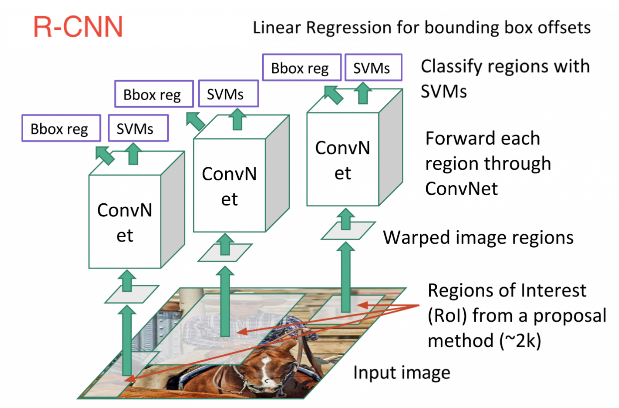
\includegraphics[width=0.7\textwidth]{figures/Estado_arte/rcnn.png}
		\caption{Fases de \acrshort{rcnn}}
		\label{fig.rcnn}
		\end{center}
\end{figure}

Fast \acrshort{rcnn} es una versión más rápida que \acrshort{rcnn}, en la que se modifican algunos aspectos para conseguirlo:
\begin{enumerate}
    \item Antes de extraer las regiones de interés se extraen las características. Para ello se emplea una única \acrshort{cnn} para toda la imagen en vez de 2000.
    \item \acrshort{svm} se remplaza por la función de softmax.
\end{enumerate}

\begin{figure}[H]
  \begin{center}
    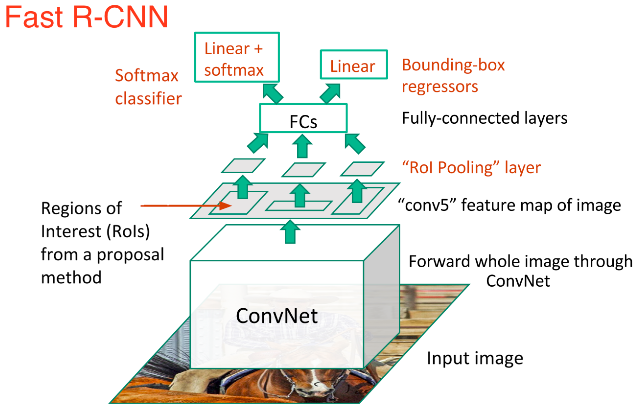
\includegraphics[width=0.7\textwidth]{figures/Estado_arte/fast_rcnn.png}
		\caption{Fases de Fast \acrshort{rcnn}}
		\label{fig.fast_rcnn}
		\end{center}
\end{figure}

Ignacio Arriola~\cite{tesis_ignacio_arriola} hace uso de Faster \acrshort{rcnn}, una versión aún más rápida que Fast \acrshort{rcnn}.




\section{Clasificación de vehículos}

La clasificación de vehículos trata de determinar a que clase pertenece cada objeto detectado. Analizando los trabajos que se centran en este problemas se ha podido ver que son tres los métodos más empleados:
\begin{itemize}
    \item Técnicas basadas en características.
    \item Técnicas basadas en modelos 3D.
\end{itemize}

Las técnicas basadas en características se centran en extraer propiedades de la imagen que permitan poder clasificar cada objeto. En el caso de la clasificación de vehículos, tratarán de definir un conjunto de características, con las cuales pueda quedar bien descrito el vehículo en cuestión. Para ello se necesitará mucha información, cuantas más características tengamos del objeto será más fácil de identificar. En esta familia de técnicas se requiere una fase de entrenamiento previa donde el sistema sea capaz de aprender las diferentes características. Una vez tengamos el sistema entrenado le pasaremos los objetos detectados, para que estime a que clase pertenecen. Dicha clase será siempre la que más características tenga en común con el objeto que pretendemos clasificar.
 
Las características pueden ser visuales o geométricas (longitud, área, relación  entre el alto y el ancho, etc). En el caso de las características geométricas Shih-Hao Yu et al.~\cite{an_Automatic_traffic} presentaron un sistema que er capaz de distinguir entre tres clases: camiones, autobuses y coches. Para ello se basaba en dos características (tamaño y linealidad). La linealidad se empleaba para distinguir entre autobuses y camiones.

Jin-Cyuan Lai, Shih-Shinh Huang and Chien-Cheng Tseng~\cite{image_based_vehicle} definieron las mismas clases que en ~\cite{an_Automatic_traffic}(coches, camiones y autobuses). Ellos se basaban en la compacidad y la proporción entre el ancho y el alto de los cuadros detectados. Además filtran los blobs en función de estas restricciones con el fin de eliminar ruido y blobs muy pequeños.

H. Asaidi , A. Aarab and M. Bellouki~\cite{shadow_elimination} definieron tres categorías: furgonetas, coches y camiones. Para definir cada vehículo determinaron 7 características geométricas. En función a estas 7 características calculaban la distancia euclídea entre el vehículo detectado y las categorías definidas. El vehículo será clasificado a la categoría con la que se obtenga una menor distancia.

Las características visuales son más complejas que las geométricas, pues tratan de definir la forma y el aspecto de cada objeto.Para ello emplean descriptores.

Dos descriptores que tienen muca relevancia son el descriptor \acrfull{hog} y el descriptor Haar. C.P. Papageorgiou, M. Oren and T. Poggio~\cite{haar_paper} fueron quien introducieron los descriptores Haar para la detección de caras humanas. Navneet Dalal and Bill Triggs~\cite{hog_paper} propusieron el descriptor \acrshort{hog} para detectar peatones.

A partir del descriptor \acrshort{hog} hay alguna variante como por ejemplo el descriptor 3DHOG. Buch et al.Buch et al.~\cite{3dhog_article}  para detectar el fondo ya emplearon este descriptor, el cual combina puntos de interés 3D y \acrshort{hog}.

Estos descriptores son muy aplicados en el mundo de la clasificación de objetos gracias a los buenos resultados que se ha visto que obtienen. \acrshort{hog} suele mezclarse con algun otro clasificador, pues se ha visto que da muy buenos resultados.

Bailing Zhang, Yifan Zhou and Hao PanTammam Tillo~\cite{hybrid_model} presentan un método basado en \acrfull{kaa} para la clasificación de vehículos. A la hora de detectar los vehículos emplean \acrshort{hog} combinado con clasificadores \acrfull{svm} en cascada. Para la clasificación también hace uso de \acrfull{eoh} como característica discriminante.

Otra técnica que ha sido aplicada a la hora de clasificar vehículos es la ténica eigenfaces, la cual fue introducida por L. Sirovich and M. Kirby~\cite{low_dimensional} para detectar y reconocer caras. Wei Wang, Yulong Shang, Jinzhi Guo and Zhiwei Qian~\cite{real_time_vehicle} fueron unos de los autores que aplicaron la técnica de eigenfaces (se trata de construir con características un subespacio de vectores) para la clasificación de vehículos. En este trabajo en concreto tan solo clasificaban las detecciones como coches o no coches. Inicialmente es necesario entrenar al sistema con una base de datos. Tras este aprendizaje ya se podrán clasificar los vehículos. Para ello se captura la parte frontal del vehículo y se le aplican operaciones de post-procesado para emplearlas en la entrada del clasificador. Esta proyección de la parte frontal del vehículo es comparada con las proyecciones recopiladas en el entrenamiento. Si la comparacion se encuentra por debajo de un umbral fijado se considerará que la clasificación se ha realizado correctamente. 

Hasta ahora hemos hablado de sistemas que empleaban o técnicas basadas en características geométricas o visuales. Las características visuales ofrecen grandes ventajas frente a las geométricas, las cuales son muy suceptibles ante cambios de posición de la cámara o vehículos con geometrías similares. Por el contrario las características visuales son muy complejas y requieren de una fase de entrenamiento. Por ello lo ideal es hacer uso de ambas características, para asi conseguir un sistema muy robusto. Dentro de este contexto tenemos a Zezhi Chen and Tim Ellis~\cite{multi_shape_descriptor}, los cuales presentan un sistema que emplea dos conjuntos de características. Uno de ellos \acrfull{mbf} formado por hasta 13 características, entre las cuales tenemos el perímetro, el área, etc. Y otro conjunto llamado \acrfull{iphog}, los cuales codifican la forma y la distribución de los objetos dentro de la imagen. Las características son introducidas en un clasificador \acrshort{svm}, el cual realiza un entrenamiento para aprender dichas características. En la Figura \ref{fig.multi_shape_descriptor} podemos ver un ejemplo de detecciones de este sistema.

\begin{figure}[H]
  \begin{center}
    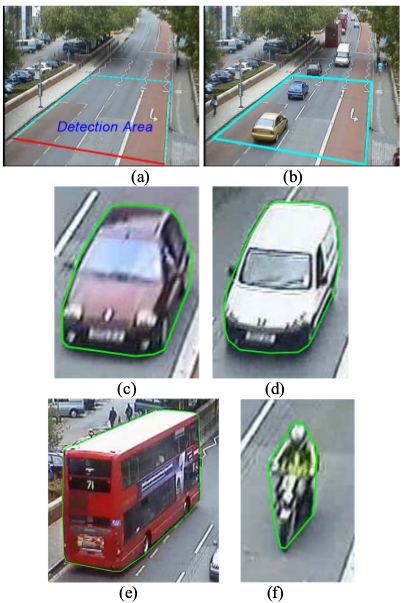
\includegraphics[width=0.4\textwidth]{figures/Estado_arte/svm_iphog.png}
		\caption{Detecciones del sistema de  Zezhi Chen and Tim Ellis~\cite{multi_shape_descriptor}}
		\label{fig.multi_shape_descriptor}
		\end{center}
\end{figure}

En las técnicas basadas en modelos 3D es necesario conocer los parámetros de la cámara que se emplee. En este caso tendremos una plantilla por cada clase y compararemos dicha plantilla con el objeto a clasificar para ver cual es la clase que más se le ajusta.
Wook-Sun Shin, Doo-Heon Song and Chang-Hun Lee~\cite{vehicle_classification_by_road} presenta  un  sistema  basado  en  plantillas  3D  que  no necesita una cámara calibrada. Este sistema se bada en los puntos de fuga de los carriles para reconstruir la forma 3D de cada vehículo. Un ejemplo de esta reconstrucción se puede ver en la Figura \ref{fig.3d_fuga}

\begin{figure}[H]
  \begin{center}
    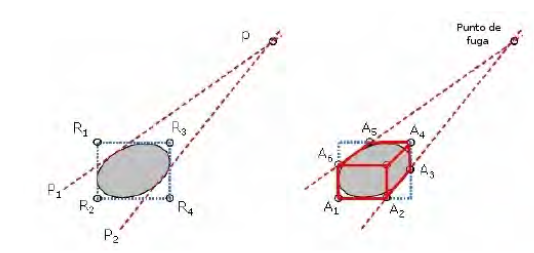
\includegraphics[width=0.6\textwidth]{figures/Estado_arte/3d_puntos_fuga.png}
		\caption{Reconstrucción 3D empleando puntos de fuga}
		\label{fig.3d_fuga}
		\end{center}
\end{figure}

Este sistema se basa en el algoritmo C4.5 de Quinlan~\cite{c4_5} a la hora de clasificar. Este algoritmo emplea la construcción de árboles de decisión para clasificar y aprender las siluetas de los vehículos. Un ejemplo de esta técnica puede verse en la Figura \ref{fig.c4_5}.

\begin{figure}[H]
  \begin{center}
    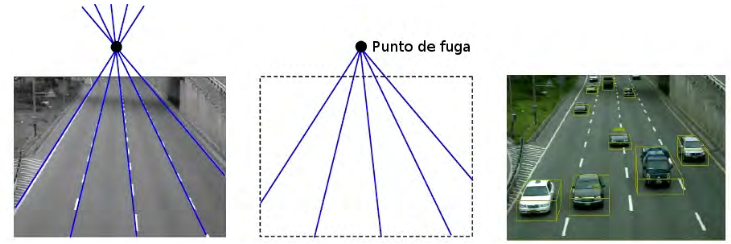
\includegraphics[width=1\textwidth]{figures/Estado_arte/c4_5.png}
		\caption{Clasificación de vehículos basada en modelos 3D construidos mediante el uso de puntos de fuga}
		\label{fig.c4_5}
		\end{center}
\end{figure}

Buch et al.~\cite{3dhog_article} presentaron un sistema que combinaba plantillas 3D con \acrshort{hog} para clasificar los diferentes vehículos y los peatones. Este sistema se llama 3DHOG, y en el aplican descriptores \acrshort{hog} a plantillas 3D que definen los vehículos. Para cada categoría se define una plantilla 3D que permita definirla. En la Figura ~\ref{fig.3dhog} se puede ver un ejemplo de dichas plantillas.

\begin{figure}[H]
  \begin{center}
    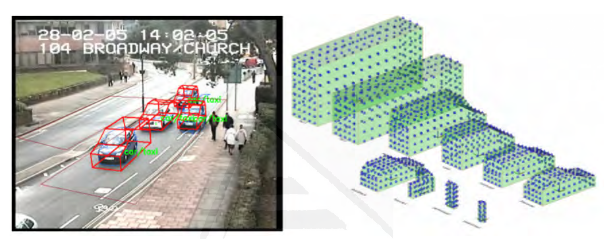
\includegraphics[width=0.8\textwidth]{figures/Estado_arte/3dhog.png}
		\caption{Plantillas 3DHOG para la clasificación de vehículos}
		\label{fig.3dhog}
		\end{center}
\end{figure}

En este sistema es necesario un previo entrenamiento. A la hora de realizar las clasificaciones se proyectan las plantillas 3D sobre los vehículos detectados y se les aplica transformaciones afines para ajustarlas al vehículo en cuestión. Tras esto se calculan sus histograma 3DHOG y se comparan con los que se han aprendido en la fase de entrenamiento. Esta reconstrucción de los histogramas 3DHOG puede verse en la Figura ~\ref{fig.3d_fuga}.

\begin{figure}[H]
  \begin{center}
    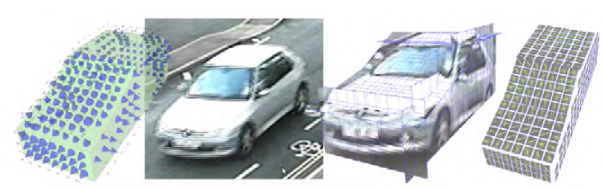
\includegraphics[width=0.7\textwidth]{figures/Estado_arte/3dhog_plantilla.png}
		\caption{Reconstrucción  del  histograma  3DHOG}
		\label{fig.3dhog_histograma}
		\end{center}
\end{figure}

Tal y como se ha comentado en la Seccion ~\ref{ap.deteccion_vehiculos} actualmente se ha extendido mucho el uso de Deep Learning tanto para la detección como para la clasificación de objetos. 
A.F. Granados y J.I. Marin.H~\cite{deteccion_flujo_vehicular} extraen los descriptores de Fourier de los vehículos detectados y los clasifican mediante una red neuronal. Dicha red neuronal consta de cuatro capas: una capa deentrada con una neurona por característica, dos capas ocultas con siete neuronas cada una y una capa de salida con una neurona clase. 


\section{Seguimiento de vehículos}

El seguimiento es la localización de un objeto a medida que va moviéndose por la imagen. Para el ser humano es una tarea muy sencilla, pero para la visión artificial se trata de un tema complejo, pues pueden cambiar muchas características en el objeto  a medida que avanza en la imagen. Tales como la forma, la iluminación, el tamaño, cambios en la perspectiva, oclusiones, movimiento de la cámara, etc.

Las técnicas más empleadas en el seguimiento de vehículos son:

\begin{itemize}
    \item Seguimiento basado en regiones
    \item Seguimiento basado en características
    \item Seguimiento basado en modelos
\end{itemize}

Las ténicas basadas en las regiones se centran en el seguimiento de regiones conexas del objeto. Normalmente la propiedad que suele emplearse es el color. En los diferentes artículos publicados se puede ver el uso de diferentes espacios de color como RGB, el espacio CEI lab o CEI LUV, el espacio HSV, etc. Lo más común es el uso de histogramas de color que nos permiten representar las regiones. Estas ténicas fueron introducidas por D. Comaniciu, V. Ramesh and P. Meer~\cite{kernel_based_object}. El seguimiento se basa en la comparación de los histogramas de las nuevas imágenes con el histograma de las regiones de interés calculadas en imágene sprevias. Para ver el parecido entre los histogramas se emplea una medida similar a la distancia de Bhattacharyya y mean-shift para optimizar la selección del candidato.

Stefan Duffner and Christophe Garcia~\cite{pixeltrack} presentó un algoritmo llamado PixelTrack, el cual combina la transformada de Hough con un modelo genérico de detección de fondo. Para ello necesita inicializar una ventana sobre el objeto. Gracias a esta técnica son capaces de seguir objetos en tiempo real con fondo cambiante, oclusiones y condiciones desfavorables.
Lili Huang and M. Barth~\cite{real_time_vehicle} plantean un algoritmo para llevar a cabo el seguimiento de vehículos y la resolución de oclusiones. En este algoritmo emplean un modelo de color basado en mean-shift para identificar a que vehículo pertenece cada parche de 3x3 píxeles cuando existe una oclusión.

El seguimiento basado en características, tal y como su nombre indica se centra en seguir los objetos en función a las características que se crean oportunas. Cada autor hace uso de unas características. Entre estas características tenemos puntos característicos como esquinas, el perímetro del objeto, sus dimensiones, etc. Si lo comparamos con el seguimiento basado en regiones podemos ver que es más robusto, pues en el caso de las regiones trataban de seguir el objeto en función del color o la textura, lo cual es muy suceptible ante el cambio de iluminación. Entre las técnicas más empleadas en este ámbito podemos encontrar \acrfull{sift}(D.G. Lowe~\cite{article_sift}), \acrfull{klt} (J. Shi and C. Tomasi~\cite{article_klt}). Otra ténica muy empelada en la literatura es \acrshort{hog}(Dalal and Bill Triggs~\cite{hog_paper}), la cual en muchas ocasiones ha sido combinada con \acrshort{svm}, tal y como se ha comentado en la seccion anterior, Zezhi Chen and Tim Ellis~\cite{multi_shape_descriptor} ya hicieron uso de ambos métodos.


El seguimiento basado en modelos trata de beneficiarse del conocimiento que tenemos de los objetos para poder realizar plantillas 2D y 3D para detectar objetos en la imagen y poder realizar su seguimiento. M.J. Leotta and J.L. Mundy~\cite{vehicle_surveillance_3d} emplean esta técnica para detectar vehículos haciendo uso de una plantilla deformable que se ajusta para identificar diferentes formas de vehículos. En la literatura también se ha combinado esta técnica con filtros de Kalman.


\section{Bases de Datos para la detección de vehículos}
\label{sec:dataset}

La detección de vehículos pretende encontrar un vehículo en una imagen o en un vídeo y determinar qué tipo de vehículo es. Dado que queremos encontrar el vehículo en cuestión bajo diferentes circunstancias, es decir, en diferentes entornos y diferentes iluminaciones, necesitaremos entrenar el modelo con un conjunto de imágenes representativo. Por este motivo, a lo largo de los últimos años han surgido diferentes datasets con el fin de solucionar este problema.

\subsection{GRAM Road-Traffic Monitoring}

GRAM Road-Traffic Monitoring (GRAM-RTM) \cite{gram-tracking} \cite{gram} es un conjunto de datos para el seguimiento de vehículos en tiempo real. Consiste en 3 secuencias de video (Figura \ref{fig.gram}), grabadas bajo diferentes condiciones y con diferentes plataformas.

El primer video, llamado M-30 (7520 \textit{frames}), se grabó en un día soleado con una cámara Nikon Coolpix L20, con una resolución de 800 x 480 @ 30 fps. La segunda secuencia, llamada M-30-HD (9390 \textit{frames}), se grabó en una ubicación similar pero durante un día nublado, y con una cámara de alta resolución: una Nikon DX3100 a 1200 x 720 @ 30 fps. La tercera secuencia de video, llamada Urban1 (23435 \textit{frames}), se grabó en una intersección concurrida con una cámara de tráfico de video vigilancia con una resolución de 600 x 360 @ 25fps.

Todos los vehículos en el conjunto de datos GRAM-RTM fueron anotados manualmente. Este conjunto posee las siguientes categorías de clases: coches, camiones, furgonetas y camiones grandes. El número total de objetos diferentes en cada secuencia es: 256 para M-30, 235 para M-30-HD y 237 para Urban1. Todas las anotaciones en el conjunto GRAM-RTM se crearon en un formato XML compatible con PASCAL VOC.

\begin{figure}
\begin{center}
	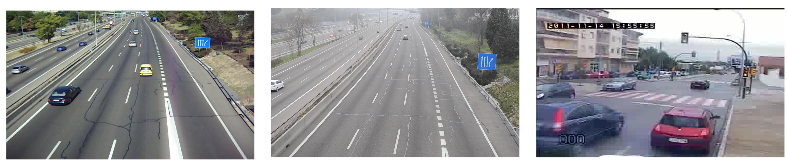
\includegraphics[width=1\textwidth]{figures/Estado_arte/gram.png}
   \caption{Imágenes de ejemplo del dataset GRAM Road-Traffic Monitoring}
	\label{fig.gram}
\end{center}
\end{figure}

\subsection{BIT-Vehicle Dataset}

El conjunto de datos BIT-Vehicle \cite{bit} contiene 9850 imágenes de vehículos. Contiene imágenes con tamaños de 1600 x 1200 y 1920 x 1080. Estas imágenes (Figura \ref{fig.bit}) fueron capturadas desde dos cámaras en diferentes momentos y lugares. Las imágenes contienen cambios en las condiciones de iluminación, la escala, el color de la superficie de los vehículos y el punto de vista. Las partes superior o inferior de algunos vehículos no están incluidas en las imágenes debido a la demora en la captura y al tamaño del vehículo. 

En cada imagen puede haber uno o dos vehículos y la ubicación de cada vehículo está previamente anotada. Además, el conjunto de datos se puede utilizar para evaluar el rendimiento de la detección de vehículos.

Los vehículos del conjunto de datos se dividen en seis categorías: bus, microbus, minifurgoneta, Sedan, SUV y camión. El número de vehículos por tipo de vehículo es de 558 para bus, 883 para microbus, 476 para minifurgoneta, 5922 para Sedan, 1392 para SUV, y 82 para camiones.

\begin{figure}[H] 
\begin{center}
	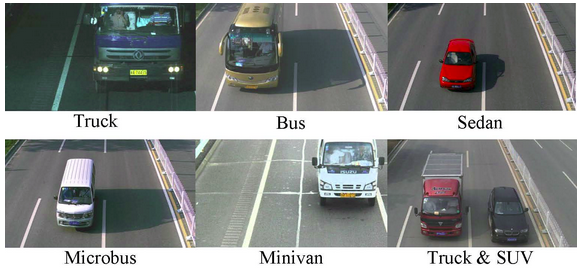
\includegraphics[width=0.9\textwidth]{figures/Estado_arte/bit.png}
   \caption{Imágenes de ejemplo del dataset BIT-Vehicle}
	\label{fig.bit}
\end{center}
\end{figure}

\subsection{CarND-Vehicle-Detection}

CarND-Vehicle-Detection \cite{carnd1} es un proyecto dedicado a la detección de vehículos en vídeo, por ello crearon dos conjuntos de datos que se pueden encontrar en \cite{carnd2}.

El \textit{dataset} 1 incluye datos de conducción en Mountain View California y las ciudades vecinas durante el día. Contiene más de 65000 etiquetas en 9423 imágenes almacenadas por una cámara de investigación Point Grey que se ejecuta a una resolución máxima de 1920x1200 a 2Hz. El conjunto de datos fue anotado mediante CrowdAI utilizando una combinación entre aprendizaje automático y el trabajo de personas. Este conjunto de datos ocupa un total de 1.5 GB, y las clases que contiene son: coche, camión y peatón.

El \textit{dataset} 2 es similar al conjunto de datos 1, pero contiene campos adicionales para la oclusión y una etiqueta adicional para los semáforos. El conjunto de datos fue anotado en su totalidad por humanos usando Autti y es un poco más grande que el anterior con 15000 imágenes (ocupa 3.3 GB). Este conjunto incluye las clases: coche, camión, peatón y farolas.
\begin{figure}[H] 
\begin{center}
	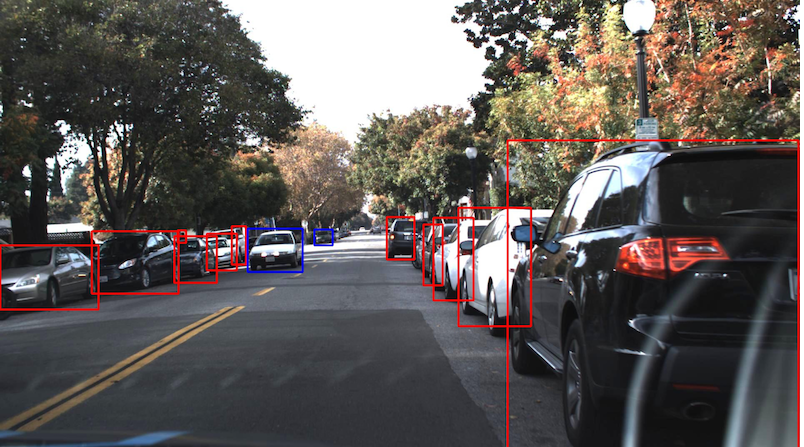
\includegraphics[width=0.8\textwidth]{figures/Estado_arte/carnd_dataset2.png}
   \caption{Imágenes de ejemplo del dataset 2 de CarND-Vehicle-Detection}
	\label{fig.carnd}
\end{center}
\end{figure}

\lhead[]{CAPÍTULO \thechapter. HERRAMIENTAS}
\chapter{Herramientas utilizadas}\label{cap.herramientas}
En este capítulo se van a explicar las diferentes bibliotecas software y entornos que se van a emplear.

Como lenguajes de programación se ha hecho uso de \textit{Python} y \textit{C++}. La aplicación se ha desarrollado casi en su totalidad en \textit{C++}, aunque la integración de \textit{TensorFlow} y \textit{Keras} se ha realizado con la versión 2.7.12 de \textit{Python}.
Para el desarrollo del modelo de \textit{Deep Learning} que se empleará para la detección, se han realizado pruebas con \textit{TensorFlow}, \textit{Keras} y \textit{Darknet}. \textit{OpenCV} se ha usado para todo lo relacionado con el tratamiento de imágenes. Finalmente la evaluación experimental de la eficacia de la aplicación desarrollada se ha realizado con la herramienta \textit{DetectionSuite}.

La interfaz gráfica de la aplicación implementada se ha hecho con \textit{gtkmm} en \textit{C++}, herramienta que permite crear interfaces de usuario con múltiples funcionalidades.



\section{DetectionSuite}
En este proyecto se ha hecho uso de la herramienta \textit{DetectionSuite}~\cite{detectionsuite} para evaluar los resultados de las redes neuronales entrenadas y de nuestra aplicación de monitorización visual de tráfico rodado.

\textit{DetectionSuite} es una herramienta que permite evaluar diferentes tipos de redes neuronales sobre un conjunto de datos. La idea es ofrecer una infraestructura genérica para evaluar los algoritmos de detección de objetos contra un conjunto de datos estandarizado y calcular las estadísticas más comunes:
\begin{itemize}
    \item \textit{\acrfull{iou}}
    \item Precisión
    \item \textit{Recall}
\end{itemize}

La \textit{\acrfull{iou}} en la detección de objetos mide la precisión de un detector en un conjunto de datos en particular y sigue la siguiente fórmula:

\begin{equation}\label{iou}
IoU = \frac{AreaofOverlap}{AreaofUnion}
\end{equation}

Donde \textit{AreaofOverlap} es el área que pertenece a la intersección entre la predicción y la realidad, mientras que \textit{AreaofUnion} es el área suma (sin repetición del solape) de la predicción y la realidad según muestra la Figura \ref{fig.formula_iou}.

En la Figura \ref{fig.ejemplo_iou} se puede ver un ejemplo visual del \textit{ground-truth} y la predicción obtenida. En este caso el \textit{AreaofOverlap} es el área que incluye únicamente la intersección entre lo que hemos predecido y el \textit{ground-truth}. Y el \textit{AreaofUnion} es el área que se forma entre el \textit{ground-truth} y la predicción.

\begin{figure}[H]
  \begin{center}
    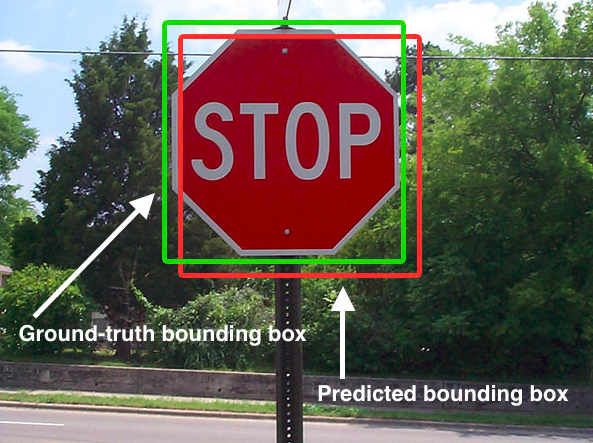
\includegraphics[width=0.6\textwidth]{figures/Herramientas/iou.png}
		\caption{Ejemplo de \acrshort{iou}}
		\label{fig.ejemplo_iou}
		\end{center}
\end{figure}


\begin{figure}[H]
  \begin{center}
    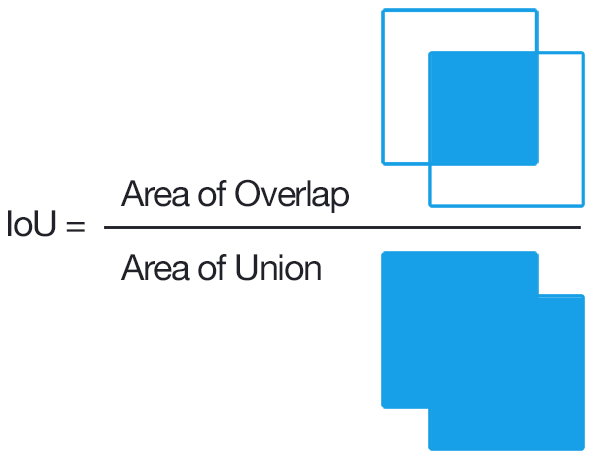
\includegraphics[width=0.4\textwidth]{figures/Herramientas/iou_formula.png}
		\caption{Fórmula \acrshort{iou}}
		\label{fig.formula_iou}
		\end{center}
\end{figure}

Antes de explicar la precisión y el \textit{recall} hay que aclarar algunos términos empleados a la hora de evaluar los resultados de las detecciones. 

\begin{itemize}
    \item \textit{True Positive (TP)}: son los verdaderos positivos, es decir aquellas detecciones que se han hecho correctamente.
    \item \textit{False Positive (FP)}: falsos positivos. Son aquellas detecciones que se han hecho pero son erróneas.
    \item \textit{False Negative (FN)}: falsos negativos. Es la proporción de casos positivos que la prueba detecta como negativos, es decir objetos que no se han detectado y deberían haberse detectado.
    \item \textit{True Negative (TN)}: verdadero negativo. Se refiere a los \textit{boundingbox} que no deben detectarse en la imagen y no se han detectado. Este valor no se emplea en las métricas.
\end{itemize}

La precisión se trata del total de detecciones correctas entre la cantidad de detecciones obtenidas. La precisión que obtiene \textit{DetectionSuite} es la promediada (\textit{\acrfull{map}}), para aquellas predicciones que tienen un \acrshort{iou} mayor que un umbral (0.5).

\begin{equation}\label{precision}
Precision = \frac{TP}{TP + FP}
\end{equation}

El \textit{recall} es la cantidad de detecciones correctas entre la cantidad de detecciones reales, es decir las detecciones del \textit{ground-truth}. Al igual que la precisión, se obtiene un promediado (\textit{\acrfull{mar}}) de las detecciones que tienen un \acrshort{iou} superior a 0.5.

\begin{equation}\label{recall}
Precision = \frac{TP}{TP + FN}
\end{equation}

Volviendo a \textit{DetectionSuite}, es una herramienta que puede emplearse tanto en Linux como en MacOS. Permite evaluar modelos entrenados en \textit{Tensorflow}, \textit{Keras}, \textit{Caffe} y \textit{Darknet}. Los formatos de \textit{dataset} que admite son:  \acrshort{yolo}, \acrshort{coco}, \textit{ImageNet Pascal VOC}, etc. A continuación se enumeran las entradas de imágenes soportadas:

\begin{itemize}
    \item WebCamera/ USB Camera
    \item Vídeos
    \item Streams from ROS
    \item Streams from ICE
    \item JdeRobot Recorder Logs
\end{itemize}

En este \acrshort{tfm} en concreto se va a hacer uso de la herramienta \textit{AutoEvaluator} de \textit{DetectionSuite}, la cual es capaz de evaluar múltiples redes en un solo conjunto de datos o múltiples conjuntos de datos en una sola ejecución. Todo lo que necesita es un archivo de configuración que contenga detalles sobre los conjuntos de datos y las redes. Los resultados se escriben en archivos CSV en el directorio de salida especificado.

\section{Entorno TensorFlow}
Para el desarrollo de la red neuronal que queremos aplicar en nuestra aplicación \textit{Smart-Traffic-Sensor} se  han probado diferentes plataformas de desarrollo de \textit{Deep Learning}, entre ellas \textit{TensorFlow} \footnote{https://www.tensorflow.org/}. Es una plataforma de código abierto \textit{end-to-end} para el \textit{Machine Learning} que fue liberada bajo licencia de \textit{Apache} 2 a finales de 2015 y que está disponible en github~\cite{github_tensorflow}. Fue desarrollada por el equipo de investigación en \textit{Machine Learning “Google Brain”}  en \textit{C++} y \textit{Python}, y es usada en multitud de productos y servicios de Google como Gmail o \textit{Google Translation}. Google ofrece en su plataforma \textit{Cloud} ejecutar \textit{Tensorflow} en \textit{Tensor Processing Unit} (TPU), un nuevo tipo de procesadores en \textit{Cloud} optimizados para ejecutar \acrfull{ia}.  \textit{TensorFlow} está orientado a problemas de \textit{Deep Learning} y permite entrenar y construir redes neuronales. 

\textit{TensorFlow} puede correr tanto en CPUs como en GPUs (haciendo uso de \textit{\acrfull{cuda}}). Está disponible en \textit{Linux} de 64 bits, \textit{MacOS}, y plataformas móviles que incluyen \textit{Android} e \textit{iOS}. Actualmente es el entorno más popular en \textit{Deep Learning}.

Puede ejecutar de forma rápida y eficiente gráficos de flujo. Un gráfico de flujo está formado por operaciones matemáticas representadas sobre nodos, y cuya entrada y salida es un vector multidimensional o tensor de datos, por este motivo recibe el nombre de \textit{TensorFlow}.

Las ventajas de este software se extienden a muchas disciplinas a parte de la tecnología TIC. Se emplea en imágenes médicas para la detección de tumores por ejemplo, también se usa en la detección y combinación de estilos artísticos en la pintura, etc.

En este \acrshort{tfm} se emplea la versión 1.12.0 de \textit{Tensorflow}.

\section{Entorno Keras}

Al igual que se ha empleado \textit{TensorFlow} como plataforma de desarrollo de la red neuronal, se ha hecho uso de \textit{Keras} \footnote{https://keras.io/}. Es un entorno de alto nivel para el aprendizaje, escrito en \textit{Python} y capaz de correr sobre \textit{TensorFlow}, \acrshort{cntk}, o \textit{Theano}. Fue desarrollado con el objetivo de facilitar el proceso de experimentación en redes neuronales de forma rápida y eficiente. Puede correr tanto en CPU como en GPU. Permite crear de forma sencilla y rápida los modelos de las redes neuronales (a través de su facilidad de uso, su modularidad y su extensibilidad). Admite redes convolucionales y redes recurrentes, así como combinaciones de las dos.

Inicialmente fue desarrollada en el proyecto de investigación ONEIROS (Open--ended Neuro--Electronic Intelligent Robot Operating System). Su creador es Fran\c{c}ois Chollet, ingeniero de \textit{Google}.
En 2017, el equipo de \textit{TensorFlow} de Google decidió dar soporte a \textit{Keras} en la biblioteca de core de \textit{TensorFlow}.

Al igual que \textit{TensorFlow}, \textit{Keras} se encuentra en github~\cite{keras_github}, pues es de código abierto. 

Las principales ventajas de \textit{Keras} son que es fácil de usar, modular, y relativamente fácil de extender, haciendo muy simple su uso. Con \textit{Keras} puedes realizar redes neuronales de forma sencilla y con muy pocas líneas de código, a diferencia de \textit{TensorFlow} que es algo más complejo. 

En este proyecto se hace uso de la versión 2.2.4 de \textit{Keras}.


\section{Entorno Darknet}\label{sec.yolo}

\textit{Darknet} \footnote{https://pjreddie.com/darknet/} es un entorno para redes neuronales de código abierto escrito en C y \acrshort{cuda}. Es rápido, fácil de instalar y admite el empleo de CPU y GPU. El código se puede encontrar en github~\cite{darknet_github}.

\textit{Darknet} se creó con el fin de emplearse en el diseño, ejecución y entrenamiento de redes neuronales profundas para la clasificación y detección de objetos. Las principales ventajas de este sistema son su simplicidad en términos de uso y su tama\~{n}o reducido.

En nuestro proyecto haremos uso de \acrfull{yolo}, que es un sistema de detección de objetos que funciona sobre \textit{Darknet}. \acrshort{yolo} utiliza \textit{Deep Learning} y \acrshort{cnn} para detectar objetos, y se distingue de sus competidores porque requiere de ver la imagen una sola vez, permitiéndole ser mucho más rápido que el resto de algoritmos. Gracias a su gran rapidez es capaz de detectar objetos en tiempo real en vídeos (hasta 30 \textit{\acrshort{fps}}).

A la hora de realizar la detección, \acrshort{yolo} en primer lugar divide la imagen en una cuadrícula de SxS. En cada una de sus celdas se estiman sus N posibles \textit{bounding boxes} con sus respectivas probabilidades de acierto. Teniendo así SxSxN \textit{bounding boxes}. Aquellas predicciones que tengan una probabilidad por debajo de un umbral quedarán eliminadas. A las que superen dicho umbral se les aplicará \textit{non--max suppression}, lo cual sirve para eliminar objetos detectados por duplicado. Este proceso puede verse en la  Figura \ref{fig.yolo}.

\begin{figure}[H]
  \begin{center}
    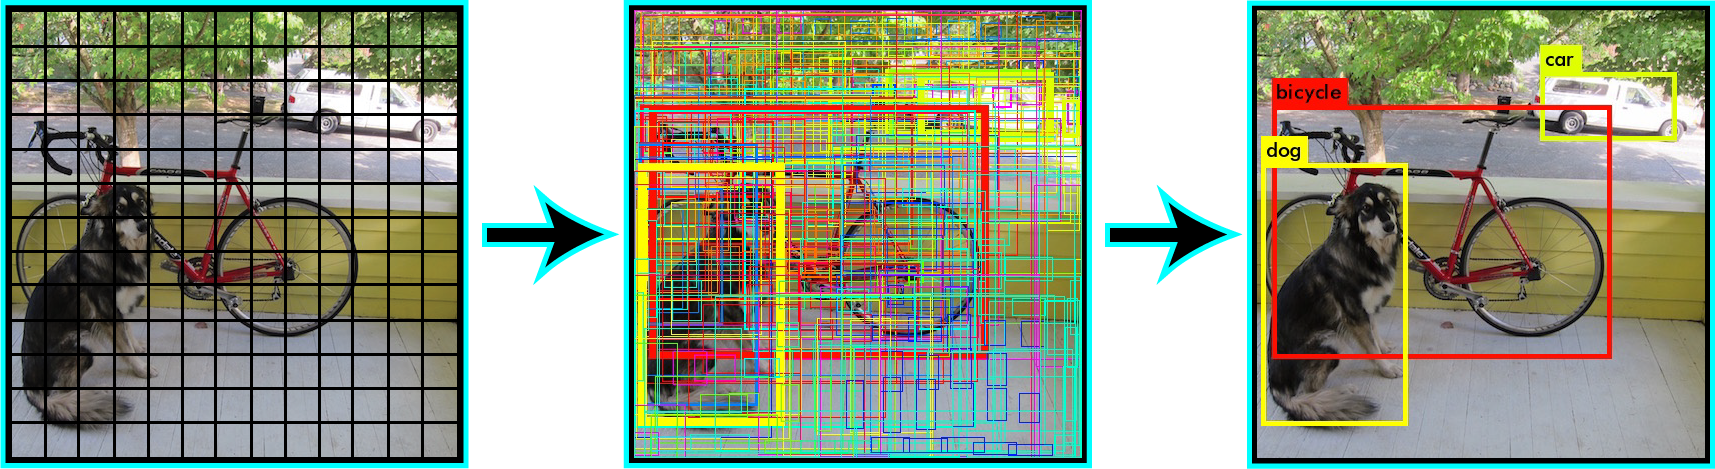
\includegraphics[width=0.9\textwidth]{figures/Herramientas/yolo.png}
		\caption{Proceso de Yolo}
		\label{fig.yolo}
		\end{center}
\end{figure}

En este \acrshort{tfm} se ha usado \textit{Darknet} para el desarrollo de una red neuronal. La versión que se ha empleado es \textit{YOLOv3}, es decir, la última versión existente hasta la fecha.

\section{Biblioteca OpenCV}

\textit{OpenCV} \footnote{https://opencv.org/} es una librería de código abierto desarrollada por \textit{Intel} y publicada  bajo licenciade BSD. Esta librería implementa gran variedad de herramientas para la interpretación de la imagen. Sus  siglas  provienen  de  los  términos anglosajones ``\textit{Open Source Computer  Vision Library}", y tal y como se puede deducir es una librería destinada a aplicaciones de visión por computador en tiempo real. Puede ser empleada en MacOS, Windows y Linux, y existen versiones para \textit{C\#}, \textit{Python} y \textit{Java}, a pesar de que originalmente era una librería en \textit{C/C++}. Además hay interfaces para \textit{Ruby}, \textit{Python}, \textit{Matlab} y otros lenguajes. 

\textit{OpenCV} implementa algoritmos para técnicas de calibración, detección de rasgos, rastreo, análisis de la forma, análisis del movimiento, reconstrucción 3D, segmentación de objetos y reconocimiento, etc. Los algoritmos se basan  en  estructuras de datos flexibles acopladas con estructuras IPL (\textit{Intel  Image Processing Library}), aprovechándose de la arquitectura de Intel en la optimización de más de la mitad de las funciones. Incorpora funciones básicas para modelar el fondo, sustraer dicho  fondo y generar imágenes de movimiento MHI  (\textit{Motion  History  Images}).  Además  incluye  funciones para determinar dónde hubo movimiento y en qué dirección. 

\begin{figure}[H]
  \begin{center}
    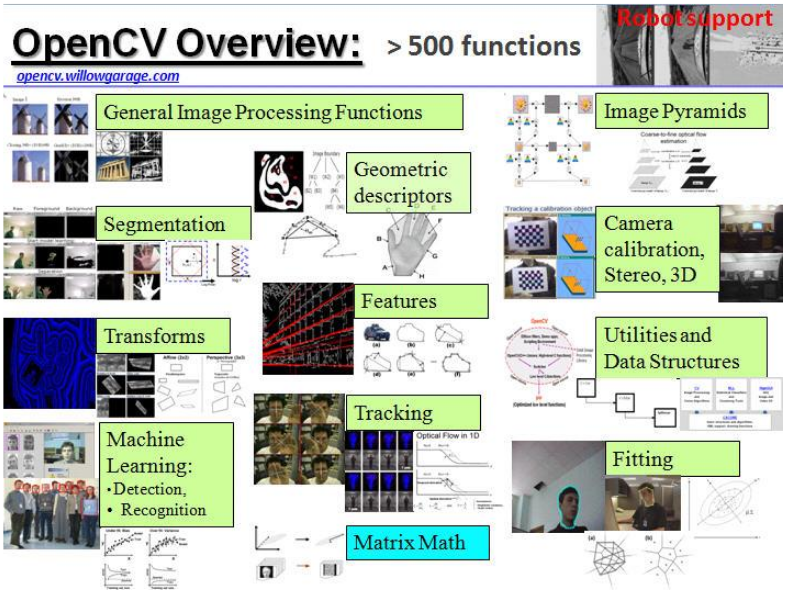
\includegraphics[width=0.6\textwidth]{figures/Herramientas/opencv.png}
		\caption{Funciones de OpenCV}
		\label{fig.opencv}
		\end{center}
\end{figure}

Fue diseñado para tener una alta eficiencia computacional, está escrito en C y puede aprovechar las ventajas de los procesadores multinúcleo. Contiene más  de  2500  funciones  que  abarcan  muchas  áreas  de  la  visión  artificial.  También  tiene  una librería   de   aprendizaje   automático   (MLL,  \textit{Machine   Learning   Library})   destinada   al reconocimiento  y agrupación de patrones estadísticos.

Desde su aparición \textit{OpenCV} ha sido usado en numerosas aplicaciones. Entre las cuales se encuentra la unión de imágenes de satélites y mapas web, la reducción de ruido en imágenes  médicas,  los  sistemas  de  detección  de movimiento,  la  calibración  de  cámaras,  el manejo  de  vehículos  no  tripulados, el  reconocimiento  de  gestos, etc. \textit{OpenCV} es empleado también en reconocimiento de música y sonido, mediante la aplicación de técnicas de reconocimiento de visión en imágenes de espectrogramas del sonido.

Hay  una  gran  cantidad  de  empresas    y  centros  de  investigación  que  emplean  estas técnicas como IBM, Microsoft, Intel, SONY, Siemens, Google, Stanford, MIT, CMU, Cambridge e INRIA.

En este proyecto se hace uso de la versión \textit{OpenCV} 3.2.


\section{Biblioteca Gtkmm}

\textit{Gtkmm} \footnote{http://www.gtkmm.org} es una encapsulación en \textit{C++} de \textit{Gtk+}. Dicha encapsulación ofrece todos los beneficios de la orientación a objetos, e incorpora otras cualidades como una mejora en la comprobación de tipos, código más reducido y legible, y un menor uso de los punteros. 

Se trata de un \textit{toolkit} para desarrollar interfaces gráficas de usuario. Es un software libre distribuido bajo la Licencia Pública General Reducida de GNU (LGPL).

\textit{Gtkmm} se organiza por medio de ventanas, las cuales contienen \textit{widgets}, como por ejemplo botones, etiquetas, cuadros de texto, etc.  Para cada \textit{widget} debemos tener un objeto C++ con el cual controlar su funcionamiento, es decir si por ejemplo nuestro \textit{widget} es un botón, necesitaremos funciones para saber si se ha pulsado o no, y acerca de que realizar si se hubiera pulsado. Para todo ello se emplea un objeto de C++. 

Aunque se puede especificar el diseño y apariencia de las ventanas y \textit{widgets} con C++, resulta más conveniente usar \textit{Glade} para el diseño de la interfaz de usuario y cargarlos en tiempo de ejecución con \textit{Gtk::Builder}. Con  \textit{Glade} podemos desarrollar las interfaces de usuario, guardarlas en formato .glade y luego cargarlas desde \textit{gtkmm} empleando \textit{ Gtk::Builder}.

En este caso se hace uso de la versión \textit{gtkmm} 3.0.




\lhead[]{CAPÍTULO \thechapter. DISENO GLOBAL DEL SISTEMA}
\chapter{Aplicación Smart-Traffic-Sensor para Monitorización de Tráfico Rodado}\label{cap.diseno}

En este capítulo se hace una descripción del sistema desarrollado para llevar a cabo la monitorización visual de vehículos.

\section{Bases de Datos de Entrenamiento}

Dado que queremos encontrar los vehículos en cuestión bajo diferentes circunstancias, es decir, en diferentes entornos y con diferentes iluminaciones, necesitaremos entrenar el modelo neuronal con un conjunto de imágenes representativo. Por este motivo, a lo largo de los últimos años han surgido diferentes \textit{datasets} públicos con el fin de permitir el entrenamiento de redes neuronales. Para el caso de la detección de vehículos hay pocos \textit{datasets}, por ello ha sido necesario crear una base de datos propia que tuviera un número suficiente de muestras y una variación amplia de tipos de escenarios, de vehículos, condiciones de luz, etc.

Esta base de datos propia consta de:
\begin{itemize}
    \item La base de datos recopilada por Redouane Kachach en su tesis doctoral, para la aplicación \textit{TrafficMonitor}, que es antecesor directo de este TFM~\cite{traffic_monitor_lab}. Dicha base de datos consta de 3460 imágenes de buena calidad.
    \item La base de datos \acrfull{gram} creada por R. Guerrero-Gomez-Olmedo, R. J. Lopez-Sastre, S. Maldonado-Bascon and A. Fernandez-Caballero~\cite{guerrero2013iwinac}. Esta base de datos está formada por imágenes extraídas de tres vídeos. El primer vídeo, llamado M-30 (7520 fotogramas), se grabó en un día soleado. El segundo, llamado M-30-HD (9390 fotogramas), se grabó en una ubicación similar pero durante un día nublado. El tercero, llamado Urban1 (23435 fotogramas) se grabó en una intersección concurrida. De esta gran base de datos se emplearon 3646 imágenes del vídeo M-30-HD y 1348 del vídeo M-30.
    \item Imágenes recopiladas de cámaras en abierto de forma online durante este TFM. 615 se trataban de situaciones de lluvia y 705 de imágenes con mala calidad.
\end{itemize} 

Se ha tratado que la base de datos construida abarcara la mayor diversidad de vehículos posibles y en diferente tipos de escenarios. Hay que tener en cuenta que toda la base de datos tiene vehículos vistos por la parte trasera. En total consta de 9774 imágenes y está formada por 7 clases: \textit{Car}, \textit{Motorcycle}, \textit{Van}, \textit{Bus}, \textit{Truck}, \textit{Small-truck} y \textit{Tank-truck}.


En estas 9774 imágenes tenemos un total de 48914 muestras repartidas tal y como se muestra en la Tabla ~\ref{tabla_muestras}.

\begin{table}[htbp] 
\begin{center}
\begin{tabular}{|l|l|}
\hline
Clases & Muestras \\
\hline \hline
Car & 38976 \\ \hline
Motorcycle & 1886 \\ \hline
Van & 5631 \\ \hline
Bus & 401 \\ \hline
Truck & 963 \\ \hline
Small-Truck & 938 \\ \hline
Tank-Truck & 119 \\ \hline
\end{tabular}
\caption{Muestras de la Base de Datos}
\label{tabla_muestras}
\end{center}
\end{table}

Para intentar conseguir un sistema robusto ante diferentes condiciones, se ha han etiquetado en la base de datos imágenes en condiciones meteorológicas buenas, imágenes en condiciones meteorológicas malas (con niebla y lluvia) e imágenes de mala calidad. En la Tabla ~\ref{tabla_img_base_datos} se puede ver la cantidad de imágenes que hay para cada tipo.
\begin{table}[htb]
\begin{center}
\begin{tabular}{|l|l|}
\hline
\cline{2-2}& Nº de Imágenes\\
\hline \hline
Buena calidad & 8406 \\ \hline
Malas Condiciones Meteorológicas & 663\\ \hline
Mala Calidad & 705\\ \hline
\end{tabular}
\caption{Imágenes de la Base de Datos}
\label{tabla_img_base_datos}
\end{center}
\end{table}

En la Figura~\ref{fig.base_datos} se pueden ver algunas imágenes de nuestra base de datos.

\begin{figure}[H]
\begin{center}
	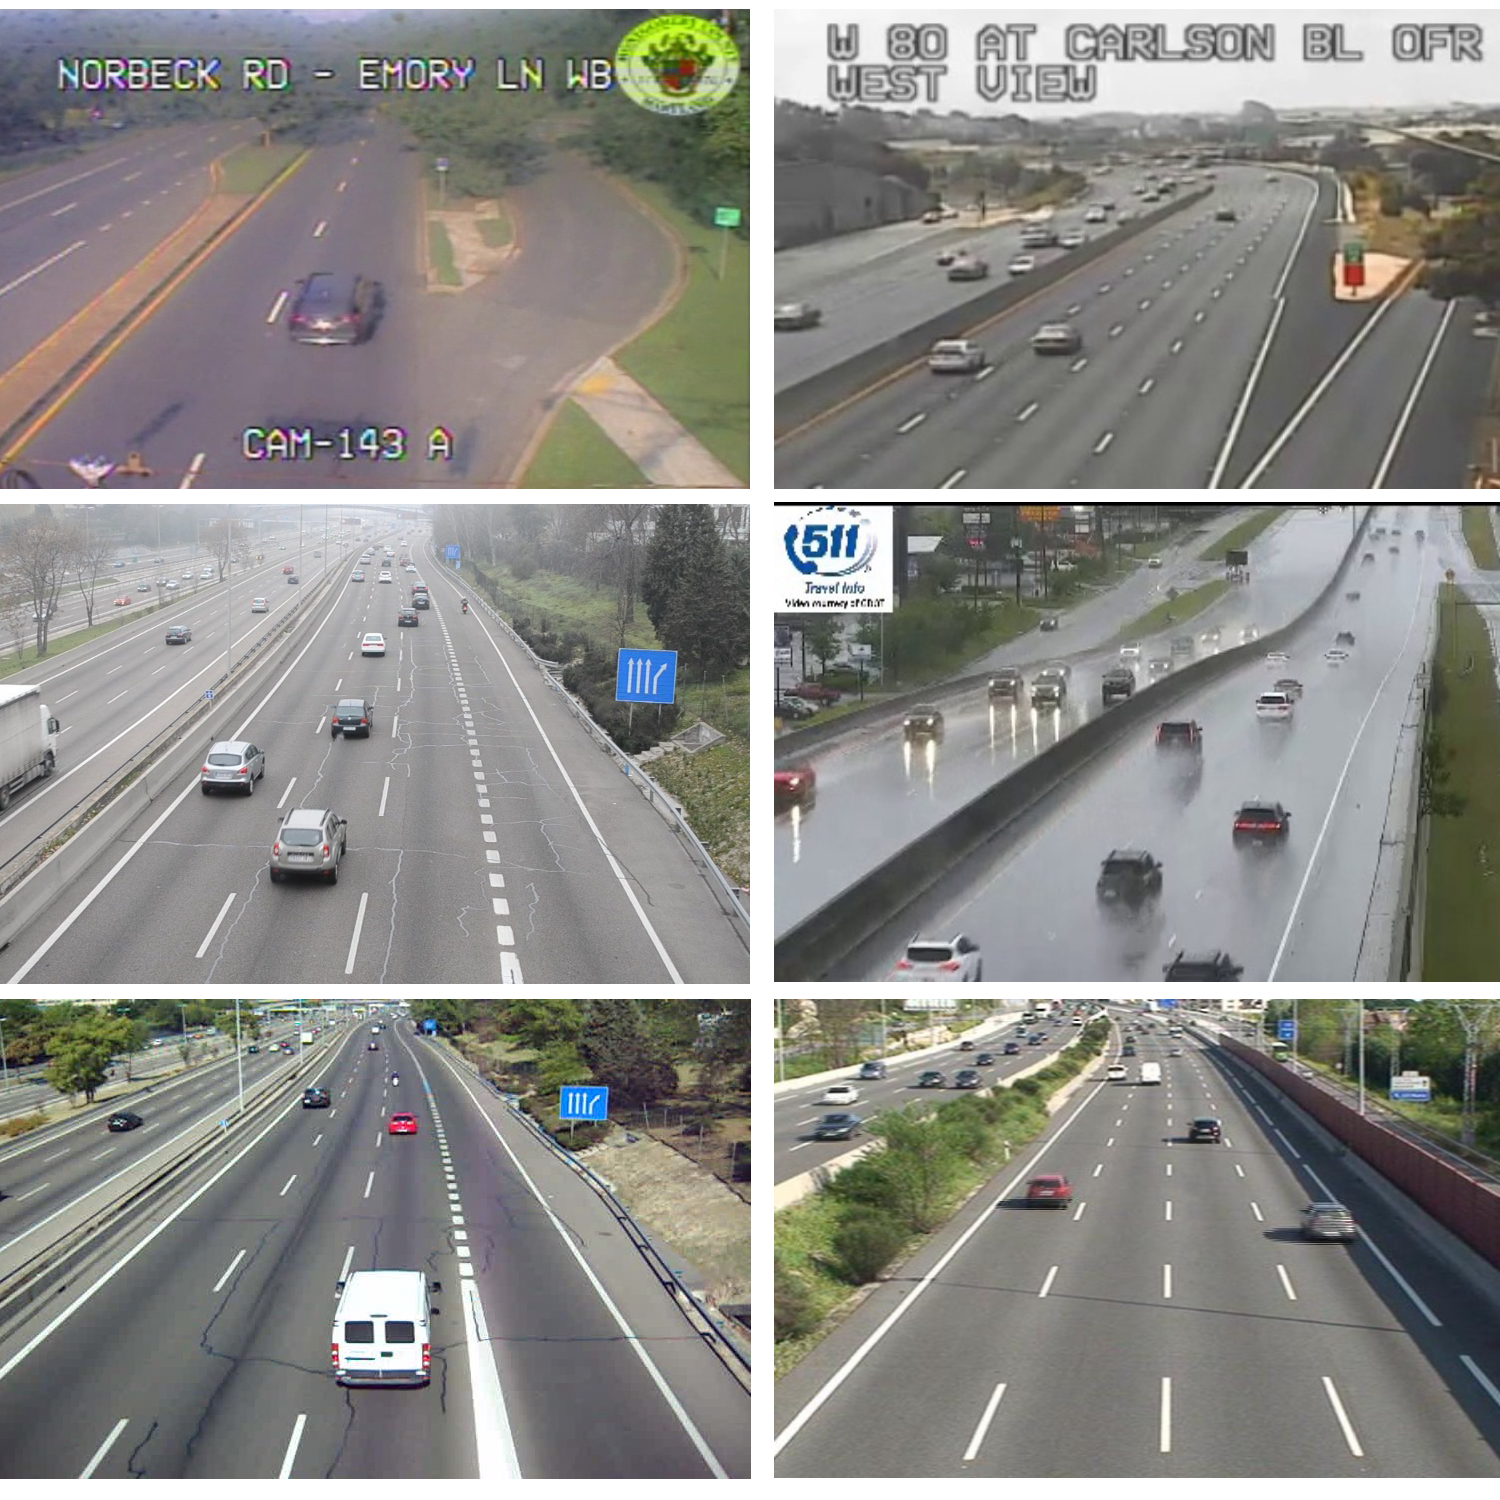
\includegraphics[width=0.6\textwidth]{figures/Diseno_global/base_datos.png}
   \caption{Base de Datos}
	\label{fig.base_datos}
\end{center}
\end{figure}

Hay que decir que todas las imágenes han sido etiquetadas a mano haciendo uso de la herramienta labelImg ~\cite{labelimg}, la cual permite guardar las etiquetas en archivos xml en formato PASCAL VOC (formato usado por ImageNet) o en formato \acrshort{yolo} en txt.

\section{Diseño de la Aplicación}

Nuestra aplicación es una especie de caja negra donde entran fotogramas de una secuencia de video y salen dichas imágenes con los vehículos detectados e identificados en función del seguimiento y la clasificación. En la Figura~\ref{fig.caja_negra} se puede ver esta caja negra.

\begin{figure}[H] 
\begin{center}
	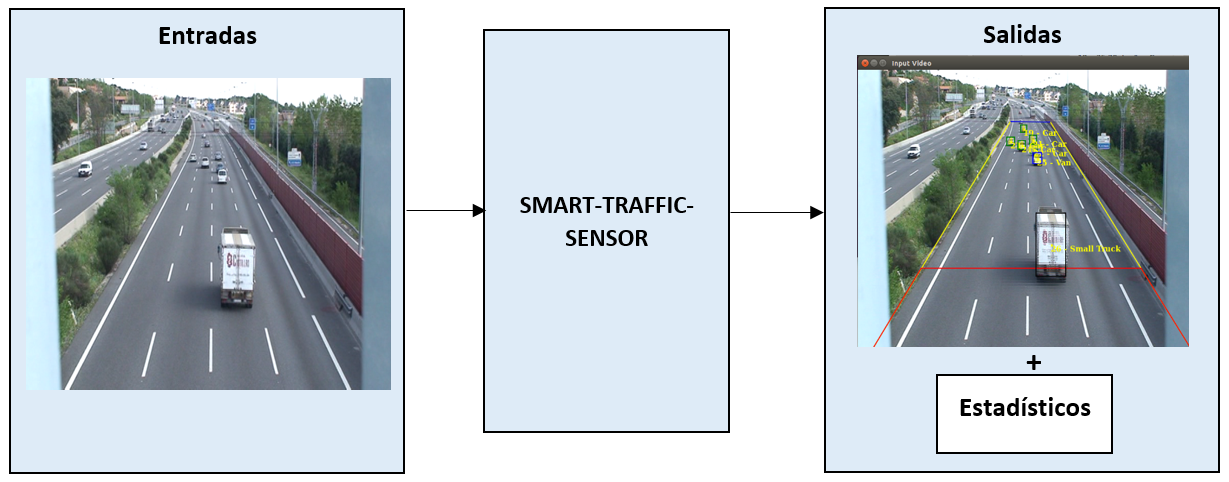
\includegraphics[width=1\textwidth]{figures/Diseno_global/caja_negra.PNG}
   \caption{Caja Negra}
	\label{fig.caja_negra}
\end{center}
\end{figure}

\textit{Smart-Traffic-Sensor} es un sistema que se realizó con el objetivo de monitorizar tráfico rodado en tiempo real. Esta monitorizacion consta de tres elementos principales:

\begin{itemize}
    \item Detección de vehículos
    \item Clasificación de vehículos
    \item Seguimiento de vehículos
\end{itemize}

En la Figura~\ref{fig.diagrama_bloques} se puede ver un diagrama de bloques que indica los elementos principales de los que se compone \textit{Smart-Traffic-Sensor}, es decir, en que se fundamenta para funcionar.

\begin{figure}[H]
\begin{center}
	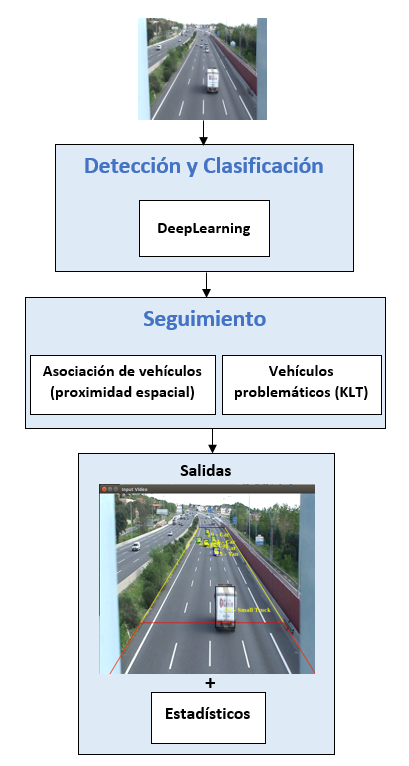
\includegraphics[width=0.5\textwidth]{figures/Diseno_global/diagrama_bloques.PNG}
   \caption{Diagrama de Bloques}
	\label{fig.diagrama_bloques}
\end{center}
\end{figure}

Las detecciones y la clasificación van de la mano, pues se realizan con \textit{Deep Learning}. En concreto con una red de \acrshort{yolo}. Los vehículos que detectemos los clasificaremos en función a 7 clases:  \textit{car, motorcycle, van, bus, truck, small-truck} y \textit{tank-truck}. 
El seguimiento se centra en la proximidad espacial, y si esta falla se utIliza \acrshort{klt}. A todos los \textit{blob} detectados se les realizará un seguimiento a lo largo del tiempo. 

El sistema del que partíamos (\textit{Traffic-Monitor}~\cite{traffic_monitor_redo}) definía en la imagen una zona de entrada y otra de seguimiento. Esto puede verse en la Figura ~\ref{fig.zonas}.

\begin{figure}[H] 
\begin{center}
	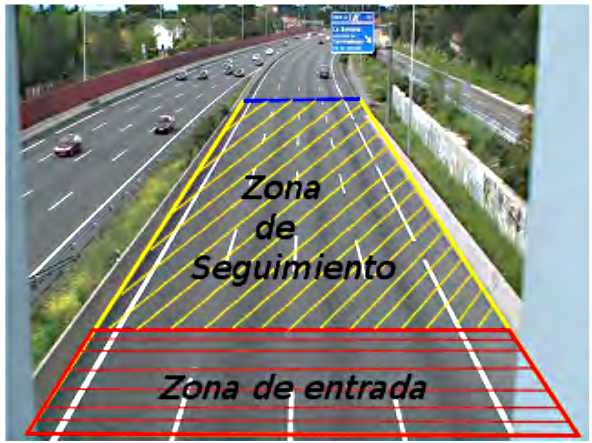
\includegraphics[width=0.5\textwidth]{figures/Diseno_global/zonas.jpg}
   \caption{Zonas de entrada y seguimiento}
	\label{fig.zonas}
\end{center}
\end{figure}

En la zona de entrada se realizan las detecciones y en la de seguimiento es donde se lleva a cabo la clasificación y el tracking de los vehículos.

Este concepto de separar zona de entrada y seguimiento va a perder relevancia en nuestro sistema, pues ya no va a ser necesario hacer esta distinción. Tendremos una única zona en la que se lleve a cabo la detección, la clasificación y el \textit{tracking}. Vamos a continuar teniendo una zona marcada en la imagen para identificar en qué parte de la carretera queremos centrar nuestras detecciones (por si existiesen carriles de diferente sentido). A esta zona de detección, clasificación y seguimiento vamos a llamarle zona de evaluación. En la Figura ~\ref{fig.nueva_zona} se puede ver la zona  de evaluación.

\begin{figure}[H] 
\begin{center}
	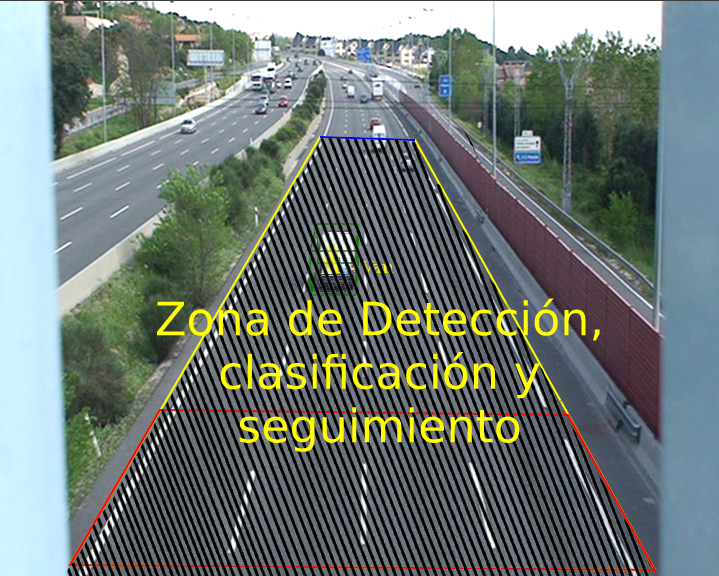
\includegraphics[width=0.5\textwidth]{figures/Diseno_global/nueva_zona.png}
   \caption{Zona Evaluación}
	\label{fig.nueva_zona}
\end{center}
\end{figure}


Este trabajo se ha basado principalmente en el uso de \textit{Deep Learning} para la clasificación y detección de vehículos. Además se ha apoyado en \acrfull{klt}, en los casos que pudiera haber pérdidas en la detección debido a oclusiones, o cuando los vehículos se encontraban muy alejados. Es decir, se ha apoyado en \acrshort{klt} cuando las condiciones a la hora de detectar eran algo complejas y por tanto el \textit{Deep Lerning} no era capaz de realizar correctamente la detección.

A la hora de realizar el \textit{tracking} se hace uso de la proximidad espacial, pero esto se explicará con más detalle en las siguientes secciones.


En resumen se puede decir que tenemos dos grandes bloques:
\begin{itemize}
    \item Detección y Clasificación de vehículos: para llevarlo a cabo se invoca a una red \acrshort{yolo} sobre la imagen completa. Dicha red fue entrenada con una base de datos propia de 9246 imágenes, las cuales fueron etiquetadas a mano.   
    \item Tracking de vehículos: se basa en la proximidad espacial para emparejar cada vehículo detectado con los vehículos detectados del instante anterior. Si un vehículo de los que está registrado no fuera detectado mediante \textit{Deep Learning} en el instante actual se haría uso de \acrshort{klt} para estimar su posición. \acrshort{klt} permite determinar el movimiento de un objeto dentro de una secuencia de imágenes.
\end{itemize}

El conjunto total de detección, clasificación y seguimiento de vehículos tarda 50 ms, con lo cual se podría esperar que la aplicación funcione a unos 20 fotogramas por segundo. Las pruebas fueron realizadas mediante un servidor por lo que el tiempo de actualización de los gráficos es mayor, obteniendo con ello que \textit{Smart-Traffic-Sensor} funciona a 10 fotogramas por segundo. No obstante esto debería probarse con un ordenador con GPU propia para ver realmente la velocidad a la que funciona. Todo esto se comentará más a fondo en el Capítulo \ref{cap.experimentos}.

A continuación se muestran dos diagramas de flujo, en los cuales se indica el planteamiento que se ha llevado a cabo en \textit{Smart-Traffic-Sensor}. En el primer diagrama~\ref{fig.diagrama_flujo_blob} se indica los pasos que se realizan una vez hemos detectado un blob en la imagen. En el segundo~\ref{fig.diagrama_flujo_vehiculos} se muestra que es lo que se hace con los vehículos ya registrados, es decir, con los que se les está llevando un seguimiento.

\begin{figure}[H] 
\begin{center}
	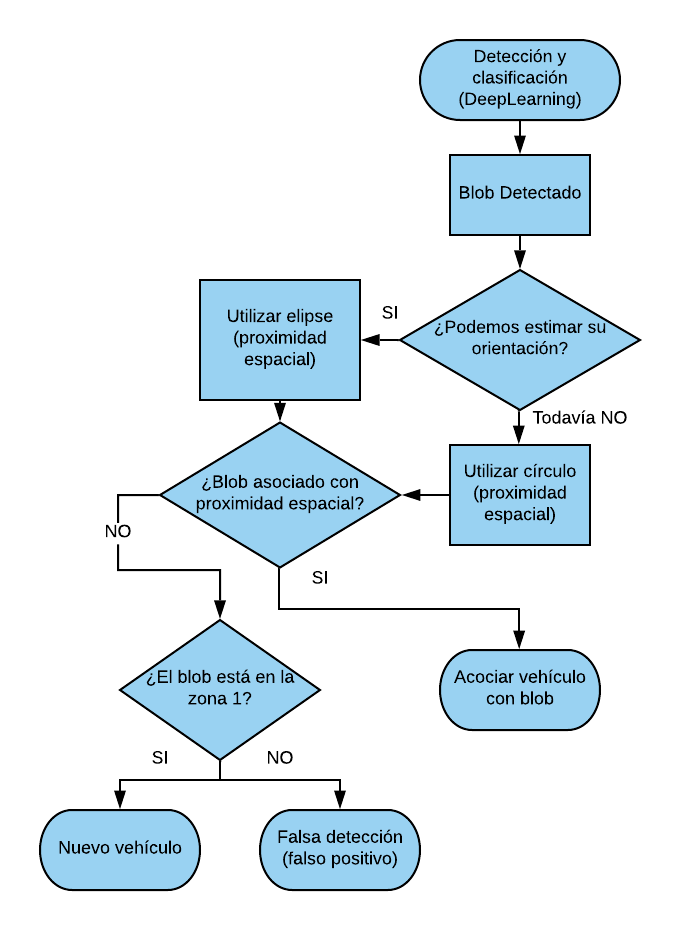
\includegraphics[width=0.8\textwidth]{figures/Diseno_global/diagrama_flujo.png}
   \caption{Diagrama de Flujo de  los Blobs Detectados}
	\label{fig.diagrama_flujo_blob}
\end{center}
\end{figure}

\begin{figure}[H] 
\begin{center}
	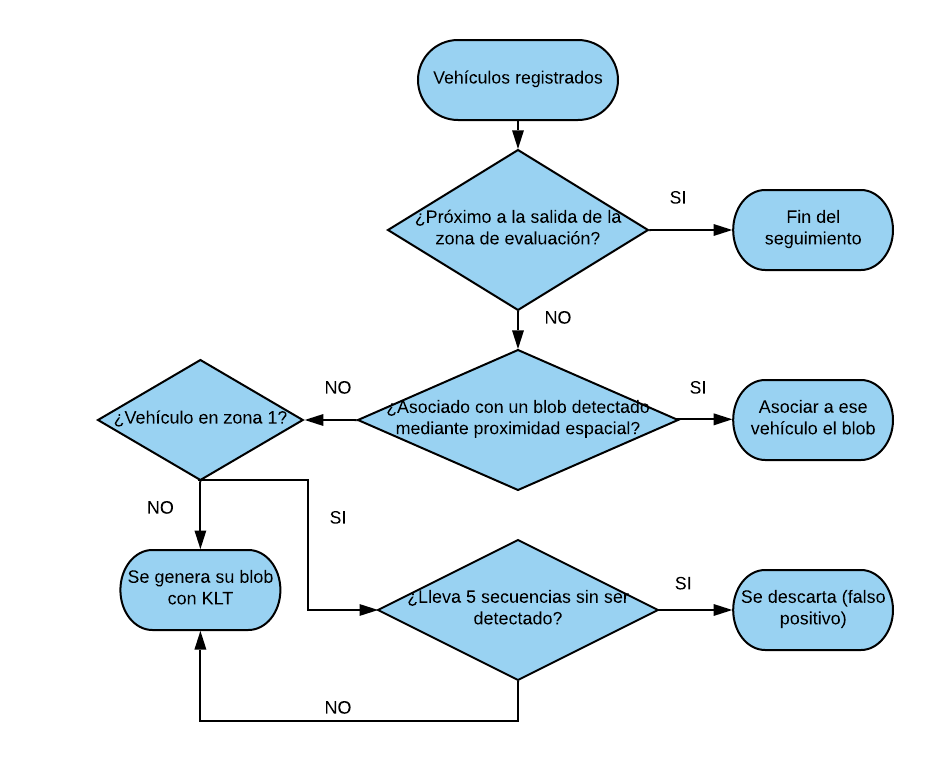
\includegraphics[width=0.9\textwidth]{figures/Diseno_global/diagrama_flujo1.png}
   \caption{Diagrama de Flujo de  los Vehículos Registrados}
	\label{fig.diagrama_flujo_vehiculos}
\end{center}
\end{figure}

\section{Detección y Clasificación}

Nuestro sistema toma como imágenes de entrada las adquiridas del vídeo que se esté monitorizando. Dichas imágenes pasan como entrada a la red neuronal, donde se detecta y clasifican los diversos vehículos. Toda la información se almacena en cada instante, para así poder realizar el tracking en función de la información registrada del instante anterior.

Tal y como ya se ha comentado anteriormente se ha hecho uso de \textit{Deep Learning}. En concreto se ha diseñado un sistema capaz de soportar redes neuronales entrenadas con diferentes \textit{frameworks} (\textit{TensorFlow}, \textit{Darknet} y \textit{Keras}) con el objetivo de detectar y clasificar los diferentes vehículos que aparezcan en la imagen. Con ello se ha pretendido realizar un sistema multiplataforma, el cual pueda adaptarse a los avances futuros de los diferentes entornos de \textit{Deep Learning}. Esto hace que nuestra aplicación no quede limitada ante la evolución de las redes neuronales.

En vídeos en carretera es muy probable que tengamos oclusiones y por supuesto vehículos que se vayan alejando, los cuales son bastante complejos de detectar. Para solventar esto nos hemos apoyado en \acrfull{klt}. Por tanto tenemos un sistema que complementa \textit{Deep Learning} con \acrshort{klt}. 

Para tener un sistema lo más robusto posible se han tenido en cuenta varios detalles:

\begin{itemize}
    \item Dentro de la zona de evaluación tenemos dos zonas. En la
     Figura ~\ref{fig.zona_evaluacion} quedan identificadas esas dos zonas.
    \begin{figure}[H] 
\begin{center}
	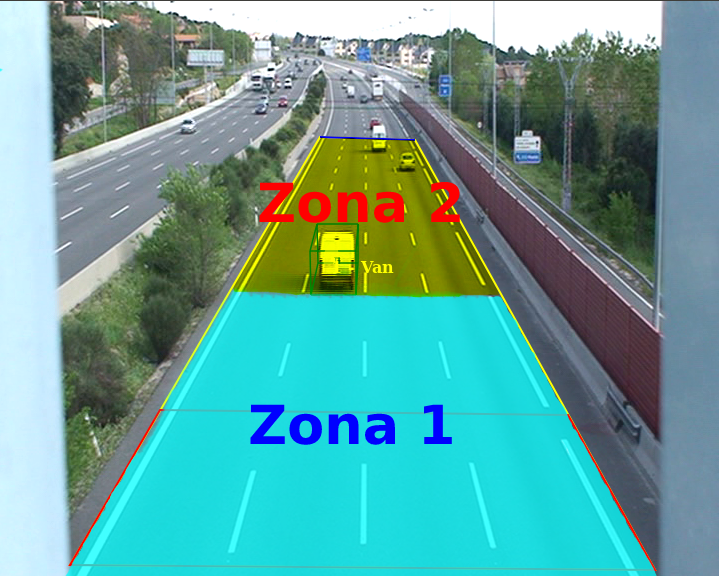
\includegraphics[width=0.7\textwidth]{figures/Diseno_global/zonas_evaluacion.png}
   \caption{Zonas identificadas en la zona de Evaluación}
	\label{fig.zona_evaluacion}
\end{center}

\end{figure}
    La zona 1 se corresponde con la mitad de la zona de evaluación por donde entran los vehículos. En esta zona es más sencillo detectar y clasificar los vehículos pues tienen mayor tamaño. La zona 2 hace referencia a la mitad por la que salen los vehículos, la cual es más compleja, pues los vehículos tendrán menor tamaño.
    \item Un vehículo siempre va a entrar a la zona de evaluación por la parte de entrada. Nunca puede aparecer de repente. Por ello no puede aparecer ningún vehículo nuevo en el medio de la carretera, es decir nunca se podrá estimar que se ha detectado un vehículo nuevo en la zona 2.
    \item Si en la zona 1 un vehículo no es detectado durante 5 secuencias seguidas se dará por hecho que ha sido un falso positivo y por tanto quedará descartado.
    \item Todo vehículo que se encuentre en la zona 2 se considerará que es un vehículo correcto. Si mediante \textit{Deep Learning} no somos capaces de detectar dicho vehículo, emplearemos \acrshort{klt} para localizarlo. 
\end{itemize}

En resumen, hay que tener en cuenta que no pueden aparecer vehículos nuevos en medio de la imagen, por tanto si esto sucede se considerará un falso positivo y se descartará. Otro aspecto que hay que tener en cuenta es que se podría dar una detección errónea, por ello si durante 5 secuencias seguidas un vehículo no ha sido detectado en la zona 1 se considerará como que era un falso positivo y se dejará de hacer su seguimiento.

Se han probado tres entornos diferentes para evaluar cual era el que mejores resultados obtenía. Para ello se hizo un primer entrenamiento con imágenes únicamente de buena calidad con el fin de determinar cual era el \textit{frameworks} que mejor funcionaba.


En los siguientes puntos se va a explicar el diseño que se ha llevado a cabo para integrar cada plataforma, en la aplicación \textit{Smart-Traffic-Sensor}.

\subsection{Entorno TensorFlow y red SSD MobilenetV2}

Para dar soporte dentro de la aplicación a redes de \textit{TensorFlow} se ha hecho uso del \textit{github models} de \textit{TensorFlow} ~\cite{tensorflow_models}, con el cual podemos entrenar una red pre-entrenada con nuestra propia base de datos. En este caso se ha empleado una red \acrfull{ssd} Mobilenet V2 entrenada con \acrshort{coco}, pues proporciona una buena relación entre la velocidad y la precisión. Para emplear dicha red se ha usado un archivo de configuración llamado \textit{ssd\_mobilenet\_v2\_coco.config}~\cite{ssd_mobilenetv2_config}.

La red \acrshort{ssd} MobileNet V2 es una red \acrshort{ssd} que en lugar de tener una red VGG-16 de base, tiene una red MobileNet. En la Figura ~\ref{fig.ssd_mobilenet} se puede ver dicho diseño.

\begin{figure}[H] 
\begin{center}
	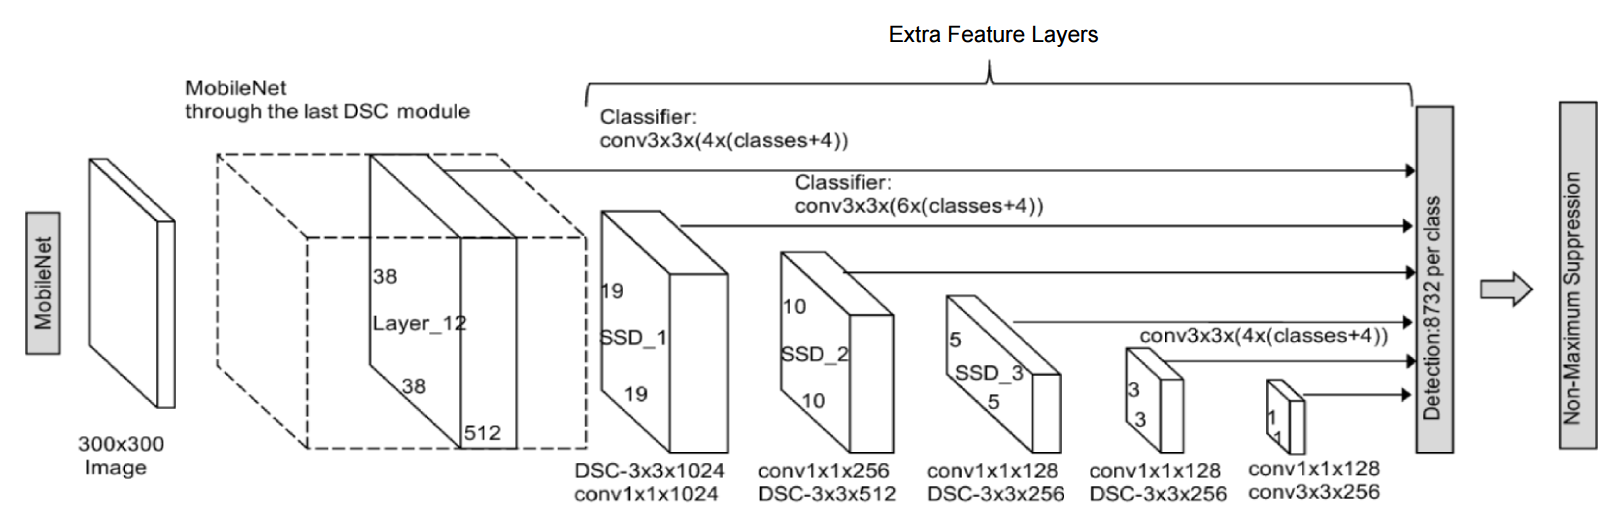
\includegraphics[width=1\textwidth]{figures/Diseno_global/ssd_mobilenet.png}
   \caption{Red \acrshort{ssd} Mobilenet V2}
	\label{fig.ssd_mobilenet}
\end{center}
\end{figure}

La primera parte de la red es la Mobilenet V2, en la cual se obtienen los mapas de características para poder realizar la clasificación y detección en las capas posteriores. 

\acrshort{ssd} ~\cite{ssd_article} es un método de detección de objetos en imágenes empleando una única red neuronal profunda. \acrshort{ssd} proporciona una gran ganancia de velocidad frente a Faster \acrshort{rcnn} \cite{rcnn_faster}, que funciona a una tasa de 7 fotogramas por segundo. El enfoque de \acrshort{ssd} se basa en una red convolucional \textit{feed-forward} que produce un conjunto de \textit{bounding boxes} de tamaño fijo y puntúa la presencia de instancias de clase de objeto en esos \textit{bounding boxes}. Tras esto realiza \textit{non-maximum suppression} para producir las detecciones finales. 

Dada una imagen de entrada y un conjunto de etiquetas de \textit{ground truth}, \acrshort{ssd} realiza el siguiente proceso:
\begin{enumerate}
\item La imagen pasa a través de una serie de capas convolucionales, produciendo varios conjuntos de mapas de características a diferentes escalas.
\item Para cada ubicación en cada uno de estos mapas de características, emplea un filtro convolucional de 3x3 para evaluar un pequeño conjunto de \textit{bounding boxes} por defecto.
\item Para cada \textit{bounding box} predice simultáneamente el desplazamiento del \textit{bounding box} y las probabilidades de clase.
\item Durante el entrenamiento hace que coincida el \textit{bounding box} del \textit{ground truth} con los \textit{bounding boxes} predichos según \textit{\acrfull{iou}}. El mejor \textit{bounding box} predicho se etiquetará como "positivo", junto con todos los demás \textit{bounding boxes} que tengan un ratio de \textit{Intersection over Union} con el \textit{ground truth} mayor de 0.5.
\end{enumerate}

\acrshort{ssd} parece sencillo, pero el entrenamiento tiene un desafío único. Clasificamos y estimamos \textit{bounding boxes} desde cada posición en la imagen, usando múltiples formas diferentes, en diferentes escalas. Como resultado, generamos un número mucho mayor de \textit{bounding boxes} que en otros modelos, y casi todos ellos son ejemplos negativos. Esto introduce un desequilibrio significativo entre los ejemplos de entrenamiento positivos y negativos.

Para solucionar este desequilibrio \acrshort{ssd} hace dos cosas. En primer lugar, utiliza la \acrfull{nms} para agrupar \textit{bounding boxes} muy superpuestos en un solo \textit{bounding box}. En otras palabras, si cuatro \textit{bounding boxes} de formas, tamaños, etc. similares contienen el mismo objeto, el \acrshort{nms} conservará el que tenga la mayor confianza y descartará el resto. En segundo lugar, el modelo usa una técnica llamada minería negativa para equilibrar las clases durante el entrenamiento. En la minería negativa dura, solo se utiliza un subconjunto de los ejemplos negativos con la mayor pérdida de entrenamiento (es decir, falsos positivos) en cada iteración de entrenamiento. \acrshort{ssd} mantiene una relación de 3: 1 de negativos a positivos.


Mobilenet emplea unas capas llamadas \textit{depthwise separable convolutions} en lugar de capas convolucionales para la clasificación. En una capa convolucional se extrae información mediante \textit{kernels} que recorren toda la imagen. Estos \textit{kernels} necesitan tener la misma profundidad que la imagen para ser aplicados, es decir, si tenemos una imagen RGB necesitaremos 3 \textit{kernels}, uno por cada canal de color. Las capas \textit{depthwise separable convolutions} siguen un proceso diferente a las convolucionales: 

\begin{enumerate}
    \item Realizan la operación \textit{depthwise convolution}, en la cual se aplican \textit{kernels} de igual profundidad que la imagen. Cada \textit{kernel} se aplica en cada canal de color por separado.
    \item Se lleva a cabo la operación \textit{pointwise convolution} en la cual se aplica un \textit{kernel} de 1x1xprofundidad de la imagen, con lo que se obtendrá así un único canal.
\end{enumerate}

Finalmente estos \textit{kernel} se combinan para obtener una única imagen. 
Si por ejemplo tenemos una imagen de 10x10x3 y se aplican capas convolucionales con \textit{kernels} de 3x3x3 el resultado será una imagen de 8x8x1. Si queremos aplicar 5 \textit{kernels} en total tendremos 5 \textit{kernels} de tamaño 3x3x3 que se moverán por la imagen 8x8 posiciones.

\begin{equation}\label{convolucional_formula}
N^{\circ} operaciones = 5x3x3x3x8x8 = 8640
\end{equation}

En el caso de \textit{depthwise separable convolutions} primero se realizará la operación \textit{depthwise convolution} con la cual obtendremos una imagen de 8x8x3 . Es decir, se emplearán 3 \textit{kernels}t de tamaño 3x3x1 para cada canal de color y estos \textit{kernels} se moveran 8x8 posiciones. Tras esto se aplicará la operación \textit{pointwise convolution}, en la cual se usará un \textit{kernel} de tamaño 1x1x3 para obtener finalmente una imagen de 8x8x1. Si tuvieramos 5 \textit{kernels} de tamaño 1x1x3 se moverán 8x8 posiciones.

\begin{equation}\label{mobilenet_formula}
N^{\circ} operaciones = (3x3x3x1x8x8) + (5x1x1x3x8x8) = 2688
\end{equation}

En conclusión, las capas \textit{depthwise separable convolutions} realizan el mismo trabajo que las convolucionales pero lo dividen en dos, consiguiendo asi reducir el número de operaciones.

Con el diseño que se ha explicado se ha entrenado un total de 3173 imágenes, de las cuales 2700 eran de \textit{train} y 473 de validación. Las imágenes de \textit{train} son las que se usan para generar el modelo. Los datos de validación seleccionan el modelo que mejores resultados obtiene.

 \subsection{Entorno Keras y red SSD VGG-16}
 
 Con \textit{Keras} se ha implementado una red \acrshort{ssd}. Para ello se ha recurrido al diseño realizados por Pierluigi Ferrari~\cite{ssd_ferrari}, el cual define una red \acrshort{ssd} que tiene como red base una VGG-16. En la Figura ~\ref{fig.ssd_300} se puede ver el diseño.
 
 \begin{figure}[H] 
\begin{center}
	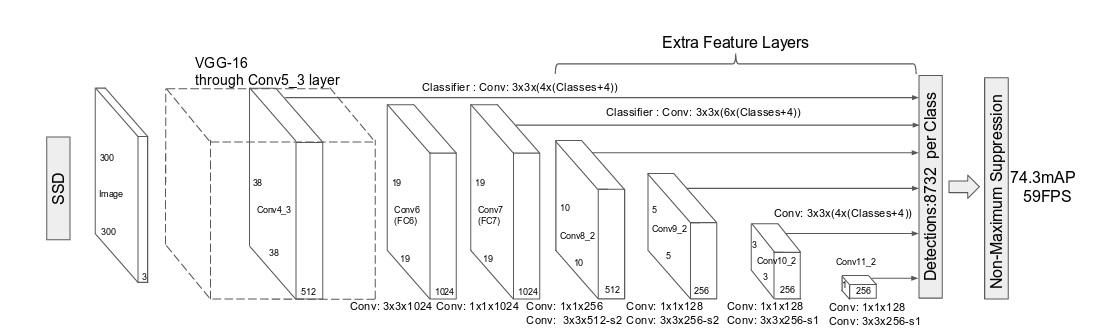
\includegraphics[width=1.1\textwidth]{figures/Diseno_global/ssd300.png}
   \caption{Red \acrshort{ssd}}
	\label{fig.ssd_300}
\end{center}
\end{figure}

VGG-16  está formada por 16 capas, de las cuales 13 son capas convolucionales, 2 capas totalmente conectadas y una capa de \textit{softmax} que se emplea para clasificar. En la Figura ~\ref{fig.vgg16} se puede ver cuál es la arquitectura de la red VGG.

 \begin{figure}[H] 
\begin{center}
	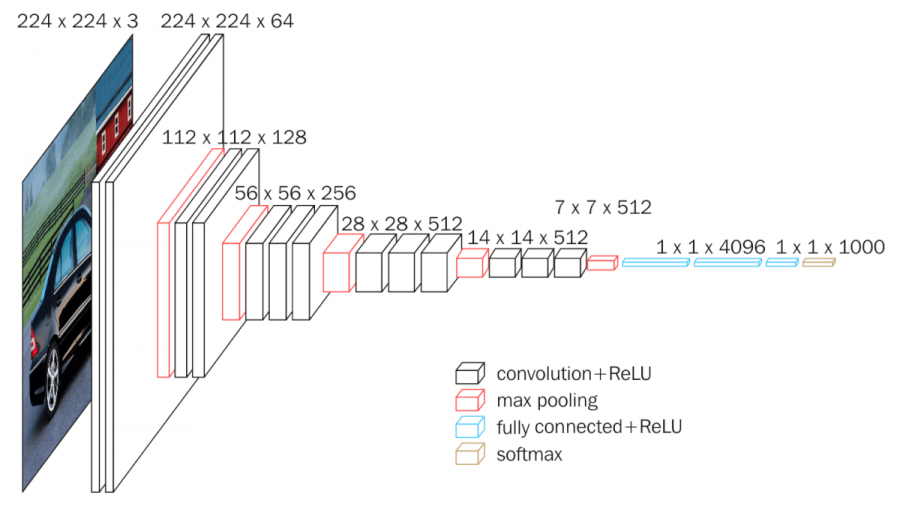
\includegraphics[width=0.8\textwidth]{figures/Diseno_global/vgg16.png}
   \caption{Red VGG-16}
	\label{fig.vgg16}
\end{center}
\end{figure}

\subsubsection{Entorno Darknet y red YOLOv3}

En este sistema se ha incluido \acrfull{yolo} debido a su gran éxito actualmente. \acrshort{yolo} ~\cite{yolo_article1} es otro enfoque para la detección de objetos. El trabajo previo a \acrshort{yolo} emplea clasificadores para realizar la detección. En esta aproximación se enmarca la detección de objetos como un problema de regresión en \textit{bounding boxes} espacialmente separados y probabilidades de clase asociadas. En la evaluación, una red neuronal única predice \textit{bounding boxes} y probabilidades de clase directamente desde imágenes completas. 

\acrshort{yolo} impone fuertes restricciones espaciales en las predicciones de los \textit{bounding boxes}, ya que cada celda de la cuadrícula solo predice dos \textit{bounding boxes} y solo puede tener una clase. Esta restricción espacial limita el número de objetos cercanos que nuestro modelo puede predecir. 

El modelo implementado es una red neuronal convolucional, donde las capas convolucionales iniciales extraen características de la imagen, mientras que las capas \textit{fully connected} predicen las probabilidades y coordenadas de salida. La red tiene 24 capas convolucionales seguidas por 2 capas \textit{fully connected}. 

La arquitectura unificada de \acrshort{yolo} (Figura~\ref{fig.yolov3}) es extremadamente rápida, procesando imágenes en tiempo real a 45 frames por segundo. Una versión más pequeña de la red, Fast \acrshort{yolo}, procesa 155 frames por segundo, logrando duplicar el \textit{\acrfull{map}} de otros detectores en tiempo real.

\begin{figure}[H] 
\begin{center}
	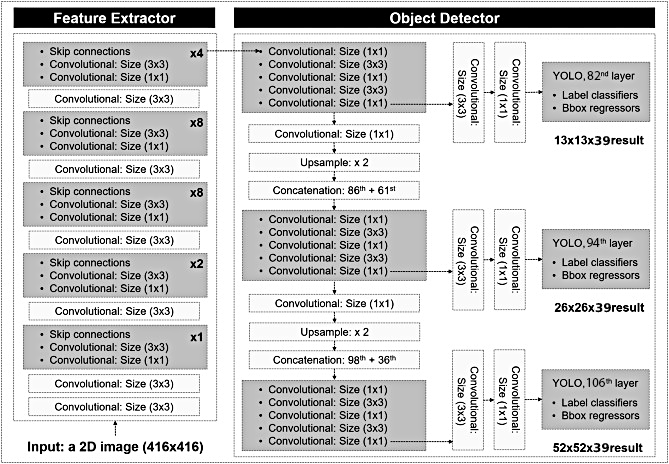
\includegraphics[width=0.9\textwidth]{figures/Diseno_global/yolov3.png}
   \caption{Arquitectura YOLO}
	\label{fig.yolov3}
\end{center}
\end{figure}

En comparación con los sistemas de detección más modernos, YOLO comete más errores de localización (especialmente con objetos pequeños), pero es menos probable que prediga falsos positivos en el fondo. Finalmente, \acrshort{yolo} aprende representaciones muy generales de objetos. Supera a otros métodos de detección, como DPM y \acrshort{rcnn}, en imágenes naturales y trabajos artísticos.


\section{Seguimiento de Vehículos}\label{sec.seguimiento}

Una vez tenemos los vehículos detectados y clasificados debemos realizar su seguimiento a lo largo de la carretera. Es decir, tenemos que asociar cada \textit{blob} detectado a los \textit{blob} anteriores de los que ya se llevaba un seguimiento. El algoritmo empleado para realizar este \textit{tracking} está basado en la proximidad espacial y \acrshort{klt}. 

\subsection{Emparejamiento por proximidad}

La diferencia de píxeles en la imagen entre la posición de un vehículo en \textit{t-1} y en \textit{t} es muy pequeña. Por tanto se puede decir que el blob de un vehículo en \textit{t} cae en una zona muy cercana al blob de ese mismo vehículo en \textit{t-1}. Esto se tendrá en cuenta a la hora de realizar el seguimiento, ya que cuando busquemos un vehículo en \textit{t} deberíamos enncontrarlo en un radio circular pequeño alrededor de la posición de ese mismo vehículo en \textit{t-1}. 

El algoritmo que se plantea en cuanto a la proximidad espacial es el empleado por Redouane Kachach en la versión anterior de la aplicación~\cite{redo_tesis}. En él se estima el área donde debería localizarse un vehículo en función de su posición en \textit{t-1}. A medida que los vehículos vayan avanzando este área se irá actualizando.

Al principio el área se toma como un círculo pues no tenemos suficientes datos acerca de su orientación. Pero a medida que el vehículo avanza y tenemos suficiente información para conocer su orientación tomaremos el área como una elipse con centro en el centro del vehículo en \textit{t-1}. 

Consideraremos que tenemos suficiente información para estimar su orientación cuando tengamos 6 posiciones de un vehículo. Se emplea regresión lineal para calcular la orientación del vehículo basándonos en la posición que va tomando el vehículo a medida que va avanzando. 

La regresión lineal consiste en minimizar $\sum_{i}\rho(r_i)$ , donde $r_i$  es la  distancia  con  el  i-ésimo  punto  y $\rho(r_i)$ es una función de la distancia. $\rho(r_i)$ se puede calcular como:

\begin{equation}\label{ec.regresion_lineal}
   \rho(r_i) = 2(\sqrt{1 +\frac{r^2}{2}} - 1) 
\end{equation}

Una vez tenemos información acerca de la orientación definiremos el área de búsqueda como una elipse que tiene como centro el mismo que el vehículo en \textit{t-1} y dirección la calculada con la Fórmula (~\ref{ec.regresion_lineal}).

Los emparejamientos entre los vehículos detectados en el instante \textit{t} y los blobs almacenados del instante \textit{t-1} se limita a los vehículos que caen dentro del área del círculo o la elipse que se obtiene en función de la posición del vehículo en el instante \textit{t-1}. En la Figura ~\ref{fig.area_vehiculo} se puede ver la evolución que sufre el área alrededor del vehículo a medida que avanza.

 \begin{figure}[H] 
\begin{center}
	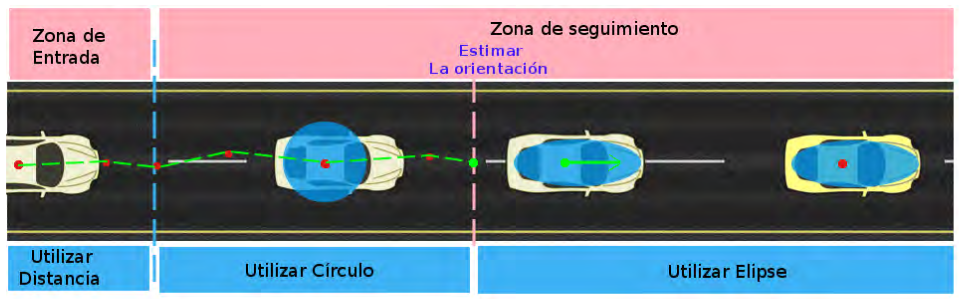
\includegraphics[width=0.9\textwidth]{figures/Diseno_global/areas_vehiculo.png}
   \caption{Evolución del área alrededor del vehículo}
	\label{fig.area_vehiculo}
\end{center}
\end{figure}


Estas elipses de definen como $C_{xc,yc,\omega}$, donde $\omega$ es la orientación y $(x_c, y_c)$ es el centro del vehículo. Además a la hora de describir una elipse debemos conocer sus dos ejes. Estos parámetros se pueden ver en la Figura ~\ref{fig.elipse}.

 \begin{figure}[H] 
\begin{center}
    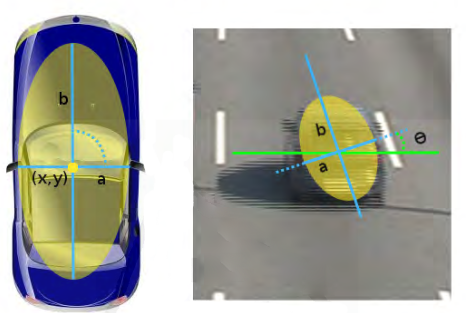
\includegraphics[width=0.7\textwidth]{figures/Diseno_global/elipse.png}
   \caption{Elipse asociada a los vehículos}
	\label{fig.elipse}
\end{center}
\end{figure}

Un blob 2D cuyo centro es $B(x,y)$ se encontrará dentro de la elipse  $C_{xc,yc,\omega}$ si se cumple:

\begin{equation}\label{ec.blob_elipse}
   C_{\omega} = \arctan(\frac{a_x}{a_y})
\end{equation}

\begin{equation} \scriptsize \label{ec.blob_elipse1}
   \left(\frac{cos(C_\omega)(B_x - C_{x_c}) + sin(C_\omega)(B_y - C_{y_c})}{a} \right)^2 + \left(\frac{cos(C_\omega)(B_y - C_{y_c}) - sin(C_\omega)(B_x - C_{x_c})}{b} \right)^2 \leq 1
\end{equation}

$a_x$ y $a_y$ son los componentes del vector de orientación. En la Figura ~\ref{fig.emparejamiento_blob} se puede ver cómo se realiza el \textit{tracking} entre dos \textit{blobs} consecutivos. 

 \begin{figure}[H] 
\begin{center}
   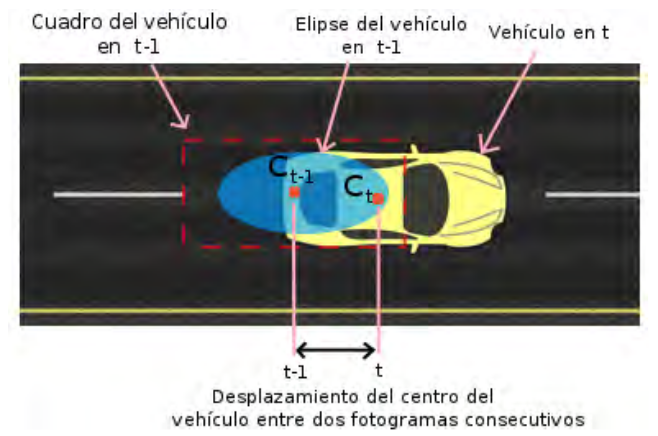
\includegraphics[width=0.7\textwidth]{figures/Diseno_global/emparejamiento_blob.png}
   \caption{Seguimiento con proximidad espacial}
	\label{fig.emparejamiento_blob}
\end{center}
\end{figure}


En la Figura~\ref{fig.proximidad_espacial} se muestra un ejemplo de \textit{Smart-Traffic-Sensor} donde se ve como se realiza el seguimiento de dos vehículos con proximidad espacial. El vehículo identificado como 2 en la imagen del instante t-1 se asocia al vehículo que se encuentra más cercano a su posición en la imagen del instante t. Lo mismo ocurre con el vehículo 3.

 \begin{figure}[H] 
\begin{center}
   \includegraphics[scale=0.3]{figures/Diseno_global/proximidad_espacial.png}
   \caption{Seguimiento con proximidad espacial \textit{Smart-Traffic-Sensor}}
	\label{fig.proximidad_espacial}
\end{center}
\end{figure}

En resumen, una detección deberá encontrarse dentro de un cierto área alrededor del \textit{blob} detectado en \textit{t-1} para poder ser identificado como el mismo vehículo. Podría darse el caso de que dos vehículos cayeran en dicho área. Por ello es necesario tener en cuenta la distancia euclídea entre el centro del blob del instante \textit{t-1} y el centro de los \textit{blob} en \textit{t}. Aquel \textit{blob} del instante \textit{t} que se encuentre a menor distancia del \textit{blob} del instante \textit{t-1} y por supuesto esté dentro del área alrededor del \textit{blob} \textit{t-1} será considerado como el mismo vehículo que el de \textit{
t-1}. Es decir si esto se cumple el \textit{blob} de \textit{t-1} y \textit{t} corresponden al  mismo vehículo pero en instantes consecutivos.

\subsection{Seguimiento por KLT}

El seguimiento se centra en asociar las detecciones actuales con los \textit{blobs} almacenados del instante anterior. En el seguimiento se tendrán ciertos aspectos en cuenta:

\begin{itemize}
    \item Si un \textit{blob} llega al final de la zona de evaluación se eliminará del seguimiento.
    \item Se recorrerán los \textit{blob} del instante \textit{t-1} almacenados con el fin de emparejarlos con los \textit{blob} detectados en el instante \textit{t}. Este emparejamiento se establecerá entre los \textit{blob} \textit{t} y \textit{t-1} que tengan menor distancia euclídea entre sus centros.
    \item Si el \textit{blob} \textit{t} asociado al \textit{blob} \textit{t-1} no cae dentro del área circular o elíptica que se genera alrededor del centro del  \textit{blob} \textit{t-1} no quedará emparejado a éste. 
    \item Si mediante proximidad espacial no somos capaces de emparejar un \textit{blob} \textit{t-1} emplearemos \acrshort{klt}.
\end{itemize}

El seguimiento se basa principalmente en la proximidad espacial pero se hará uso de \acrshort{klt} en casos problemáticos, haciendo asi más robusto nuestro sistema. \acrshort{klt} se calculará en todas las secuencias para ir actualizando los puntos característicos.

Si no se detecta un vehículo ya sea porque haya alguna oclusión o se encuentre muy lejos, se empleará \acrshort{klt}, pues se ha visto que funciona incluso ante oclusiones durante un pequeño número de fotogramas consecutivos.

Para poder realizar \acrshort{klt} necesitamos conocer el centro de masas de los vehículos y sus características visuales. En función de los puntos característicos del vehículo en \textit{t-1} , \acrshort{klt} calcula el emparejamiento para cada punto característico y como resultado genera un nuevo conjunto de puntos característicos correspondientes al vehículo en cuestión. Para llegar a conseguir un emparejamiento correcto el sistema se basa en votos de los puntos característicos que un objeto tiene asociado. 

Un ejemplo del seguimiento mediante \acrshort{klt} se puede ver en la Figura~\ref{fig.klt_deteccion}. En ella se puede ver como a pesar de haber una oclusión se sigue detectando el vehículo. En este caso \textit{Deep Learning} no era capaz de detectarlo, pero gracias al uso de \acrshort{klt} no llegamos a perderlo.

 \begin{figure}[H] 
\begin{center}
   \includegraphics[scale=0.5]{figures/Diseno_global/klt_deteccion.png}
   \caption{Seguimiento con KLT \textit{Smart-Traffic-Sensor}}
	\label{fig.klt_deteccion}
\end{center}
\end{figure}

A continuación se va a explicar más en detalle \acrshort{klt}.

Jean-Yves Bouguet~\cite{klt_bouguet} hicieron una implementación de \acrshort{klt} en la cual aplicaban \acrshort{klt} de forma recursiva sobre una pirámide de imágenes. Esta misma implementación es la que se ha empleado en este trabajo. 

Lukas Kanade es un método diferencial y local en el que se analiza la vecindad de cada píxel. En él se asume que el flujo óptico es constante en una vecindad, y se resuelve la ecuación del flujo óptico para todos los píxeles en esta vecindad por el método de los mínimos cuadrados. Para el cálculo de los vectores de velocidad se emplea la siguiente fórmula:

\begin{equation}\label{klt_formula}
   \begin{bmatrix}u \\ v\end{bmatrix} = \begin{bmatrix}
            \sum_{i}I_{xi}^2 & \sum_{i}I_{xi}I_{yi} \\
            \sum_{i}I_{xi}I_{yi} &  \sum_{i}I_{yi}^2 \\
\end{bmatrix}^{-1} \begin{bmatrix}
-\sum_{i}I_{xi}I_{ti} \\
-\sum_{i}I_{yi}I_{ti} \\
\end{bmatrix}
\end{equation}
\\

El vector $(u,v)$ es el vector de desplazamiento del flujo óptico.
$I_x$ es la media del gradiente en x entre dos imágenes consecutivas, es decir, si $I(t)$ es la imagen del instante actual e $I(t+1)$ es la imagen en el instante siguiente, la $I_x$ de estos fotogramas es:

\begin{equation}
    I_x = \frac{I_x(t)+I_x(t+1)}{2}
\end{equation}

$I_x(t)$ es el gradiente en el eje x de la imagen $I(t)$ e $I_x(t+1)$ es el gradiente en $x$ de la imagen $I(t+1)$. $I_y$ es la media de los gradientes en $y$ de la imagen $I(t)$ e $I(t+1)$:

\begin{equation}
    I_y = \frac{I_y(t)+I_y(t+1)}{2}
\end{equation}

$I_t$ es la diferencia entre $I(t)$ suavizada e $I(t+1)$ suavizada:

\begin{equation}
   I_t = I'(t+1) - I'(t) 
\end{equation}

Tal y como se ha dicho \acrshort{klt} se aplica en forma de \textit{kernels} de tamaño $\omega x \omega$ a lo largo de la imagen. El tamaño de los \textit{kernels} debe ser definido en función de la cantidad de movimiento que tenga la imagen. Un valor de \textit{kernel} pequeño será idóneo para evaluar desplazamientos pequeños de un punto. El uso de un tamaño grande de \textit{kernel} aumenta el riesgo de obtener un error, pero hay en casos en los que el desplazamiento de un punto es muy grande y esto es necesario.

En la Figura ~\ref{fig.klt_piramidal} se puede ver cómo funciona \acrshort{klt} de forma piramidal.

 \begin{figure}[H] 
\begin{center}
	\includegraphics[width=0.7\textwidth]{figures/Diseno_global/klt_piramidal.png}
   \caption{\acrshort{klt} Piramidal}
	\label{fig.klt_piramidal}
\end{center}
\end{figure}

Gracias al empleo de \acrshort{klt} piramidal se pueden estimar grandes desplazamientos con un tamaño de ventana muy pequeño.


\section{Estimación de la Velocidad}

Derivado del seguimiento de vehículos \textit{Smart-Traffic-Sensor} ofrece la funcionalidad de estimar la velocidad media que tienen estos vehículos durante su seguimiento.

\textit{Smart-Traffic-Sensor} tiene opciones para configurar la cámara, es decir para realizar su calibración. Al tener información de la cámara empleada tendremos información 3D de la imagen. Es decir podemos realizar una proyección al mundo 3D de nuestros puntos en la imagen.

Para calcular la velocidad sólo necesitamos conocer la distancia que ha recorrido el vehículo y el tiempo que ha tardado en hacerlo. Disponemos de una zona de evaluación por la cual discurren los vehículos, por tanto podemos saber cuánta distancia recorre por dicha zona de evaluación, y el tiempo que tarda en hacerlo. Para calcular la distancia tenemos que calcular la posición 3D de los vehículos y con ella hacer su diferencia. Esto se puede llevar a cabo haciendo uso de su homografía, la cual podemos estimar gracias a que conocemos los parámetros de la cámara.

\section{Interfaz Gráfica de la Aplicación}

La interfaz gráfica del proyecto nos da información acerca de lo que sucede en el vídeo que estamos monitorizando, además de mostrarnos en todo momento una ventana en la que se ve el vídeo que estamos monitorizando.

Esta interfaz gráfica tiene dos partes principales:
\begin{itemize}
    \item Una ventana denominada \textit{Input Video} en la que se ve el vídeo que evaluamos y su monitorizacion (detecciones, clasificación y seguimiento). Un ejemplo de esta ventana puede verse en la Figura~\ref{fig.input_video}.
     \begin{figure}[H] 
    \begin{center}
    	\includegraphics[scale=0.4]{figures/Diseno_global/sts_buena.png}
       \caption{Ventana \textit{Input Video}}
    	\label{fig.input_video}
    \end{center}
    \end{figure}
    \item La interfaz llamada \textit{Smart-Traffic-Sensor}, la cual controla toda nuestra aplicación y nos muestra información acerca de lo que se va registrando de la monitorización. Dicha ventana se puede ver en la Figura~\ref{fig.interfaz_sts}.
     \begin{figure}[H] 
    \begin{center}
    	\includegraphics[scale=0.5]{figures/Diseno_global/interfaz_grafica.png}
       \caption{Interfaz \textit{
       Smart-Traffic-Sensor}}
    	\label{fig.interfaz_sts}
    \end{center}
    \end{figure}
\end{itemize}

La interfaz \textit{Smart-Traffic-Sensor} nos ofrece diversas funcionalidades para modificar lo que se muestra en la ventana \textit{Input Video}, nos permite cambiar el método de detección, clasificación y seguimiento, además de mostrarnos información acerca de los vehículos que se están monitorizando.

A contiuación se va a explicar brevemente la funcionalidad de los botones que aplican en nuestro método, pues algunos solo aplican al funcionamiento del antiguo \textit{Traffic-Monitor}:
\begin{itemize}
    \item \textit{Play} permite detener y poner en marcha la ejecución del vídeo.
    \item \textit{Save} nos ofrece la posibilidad de guardar información acerca de la zona de evaluación, es decir, guardar información acerca del tamaño y los puntos en los que se encuentra la zona de evaluación.
    \item \textit{Classify} muestra los blobs y su clase (siempre que esté también activo \textit{Show Categories}).
    \item \textit{Proximity Tracking}, \textit{KLT tracking}, \textit{TensorFlow Tracking}, \textit{Keras Tracking} y \textit{Darknet Tracking} permiten cambiar de método para la detección, clasificación y seguimiento. \textit{Proximity Tracking}, \textit{KLT tracking} pertenecen al algoritmo que desarrollo Redouane en su tesis~\cite{redo_tesis}. Con \textit{Proximity Tracking} se emplea únicamente proximidad espacial para el seguimiento y en \textit{KLT tracking} se incluye \acrshort{klt} para los casos en los que la detección es insuficiente. Con \textit{TensorFlow Tracking}, \textit{Keras Tracking} y \textit{Darknet Tracking} se activa el método desarrollado en este trabajo. La única diferencia entre ellos es la plataforma de detección y clasificación.
    \item \textit{Show box} muestra el blob completamente pintado de verde. Solo aplicará si no está activo \textit{Classify}. En la Figura~\ref{fig.show_box} se puede ver un ejemplo.
        \begin{figure}[H] 
    \begin{center}
    	\includegraphics[scale=0.35]{figures/Diseno_global/show_box.png}
       \caption{\textit{Show box} activo}
    	\label{fig.show_box}
    \end{center}
    \end{figure}
    \item \textit{Show Categories} nos muestra la clase del vehículo monitorizado. Para que muestre la clase debe estar también activado \textit{Classify}.
    \item \textit{Show tracking zone} oculta o muestra la zona de evaluación.
    \textit{Show tracking info} nos permite ver en \textit{Input Video} toda la información de los vehículos monitorizados.
\end{itemize}

La interfaz también muestra un histórico de los vehículos monitorizados y una estadística total de la cantidad de vehículos de cada clase que han sido registrados. Esto puede verse en la Figura~\ref{fig.info_vehicles}.

    
Con todo ello tenemos una interfaz que nos muestra información acerca de los vehículos monitorizados muy completa.


    \begin{figure}[H] 
    \begin{center}
    	\includegraphics[scale=0.6]{figures/Diseno_global/info.png}
       \caption{Información de los Vehículos Monitorizados}
    	\label{fig.info_vehicles}
    \end{center}
    \end{figure}
    

\lhead[]{CAPÍTULO \thechapter. EXPERIMENTOS}
\chapter{Experimentos}\label{cap.experimentos}

A la hora de crear cualquier sistema es necesario hacer múltiples experimentos que nos permitan llegar a ciertas conclusiones que nos sean útiles a la hora de mejorar el diseño. Dichos experimentos deben ser evaluados de alguna forma para comprobar la calidad de los resultados que obtenemos. En este trabajo en concreto se ha recurrido a la herramienta \textit{DeepLearningSuite}~\cite{detectionsuite} para llevar a cabo dicha evaluación.

Con \textit{DeepLearningSuite} se obtienen medidas de calidad tales como la precición y el recall medios (\acrshort{map} y \acrshort{mar}) de todas las clases en función de la \acrfull{iou}. En nuestro caso nos hemos quedado con las medidas que tienen un \acrshort{iou} como mínimo de 0.5, pues se ha considerado que es suficiente para medir la calidad.

Este Capítulo vamos a dividirlo en cinco secciones en las cuales hablaremos de lo siguiente:
\begin{itemize}
    \item Evaluación de diversas redes neuronales
    \item Evaluación ampliando Dataset
    \item Evaluación de Darknet con diferentes conjuntos  de imágenes
    \item Evaluación de Smart-Traffic-Sensor
    \item Evaluación de los tiempos de procesamiento
\end{itemize}

A lo largo de este Capítulo se van a ver diferentes experimentos realizados y las medidas obtenidas con ellos en cuanto al \acrfull{map}, \acrfull{mar} con un mínimo de 0.5 \acrshort{iou}, y el tiempo de procesamiento que dedica al realizar las detecciones.

Hay que decir que todos los experimentos realizados con \textit{DeepLearningSuite} se han hecho desde un ordenador sin GPU, por ello se verá que los tiempos medios de procesamiento son un poco elevados.

\section{Evaluación de diversas redes neuronales}
 
Tal y como se ha comentado en el Capítulo~\ref{cap.diseno} se han realizado pruebas con diferentes \textit{frameworks}. En concreto con \textit{TensorFlow}, \textit{Keras}, y \textit{Darknet}. Con ello se pretendía ver cual era el framework que mejores resultados obtenía, además de dotar a \textit{Smart-Traffic-Sensor} de la capacidad de admitir redes entrenadas con diversos \textit{frameworks}.

Para llevar a cabo el entrenamiento en todos los \textit{frameworks} mencionados se han empleado un total de 3173 imágenes, de las cuales 2700 eran de \textit{train} y 473 de validación. Todas ellas en condiciones meteorológicas favorables y con buena calidad. La distribución de las muestras que posee la base de datos se indica en la Tabla~\ref{tabla_database}.

\begin{table}[H]
\begin{center}
\begin{tabular}{|l|l|}
\hline
Clases & Muestras \\
\hline \hline
Car & 15798 \\ \hline
Motorcycle & 143 \\ \hline
Van & 1437 \\ \hline
Bus & 274 \\ \hline
Truck & 765 \\ \hline
Small-Truck & 400 \\ \hline
Tank-Truck & 103 \\ \hline
Total & 18920 \\ \hline
\end{tabular}
\caption{Muestras de la Base de Datos del 1º entrenamiento}
\label{tabla_database}
\end{center}
\end{table}

En el entrenamiento se ha partido de modelos pre-entrenados. Para ver como el entrenamiento con nuestros datos consigue mejorar la capacidad de las redes a la hora de detectar objetos, se han evaluado las redes pre-entrenadas y las entrenadas. La evaluación se ha realizado sobre un conjunto de 303 imágenes, con muestras de diferentes clases de vehículos. En la Tabla~\ref{tabla_datos_primera_evaluacion} se puede ver que clases de muestras contenían las imágenes con las que se ha realizado el test.

\begin{table}[H]
\begin{center}
\begin{tabular}{|l|l|}
\hline
Clases & Muestras \\
\hline \hline
Car & 922 \\ \hline
Motorcycle & 19 \\ \hline
Van & 125 \\ \hline
Truck & 82 \\ \hline
Small-Truck & 112 \\ \hline
Total & 1260 \\ \hline
\end{tabular}
\caption{Muestras de los datos de Test de la primera evaluación}
\label{tabla_datos_primera_evaluacion}
\end{center}
\end{table}

En la Tabla~\ref{tabla_redes_preentrenadas} se pueden ver los resultados obtenidos tras evaluar las redes pre-entrenadas con algunos datos de test.
\begin{table}[H] 
\begin{center}
\begin{tabular}{|l|l|l|l|}
\hline
Redes Neuronales & mAP & mAR & Mean Inference Time (ms) \\ 
\hline \hline
Keras(VGG\_ILSVRC\_16\_layers\_fc\_reduced.h5) & 0 & 0 & 0\\ \hline
TensorFlow (frozen\_inference\_graph.pb) & 0.0035 & 0.0373 & 142 \\ \hline
Darknet  (darknet53.conv.74) & 0 & 0 & 14162 \\ \hline
\end{tabular}
\caption{Resultados Redes Pre-Entrenadas}
\label{tabla_redes_preentrenadas}
\end{center}
\end{table}

Los resultados que se obtienen con nuestras redes entrenadas se pueden ver en la Tabla~\ref{tabla_redes_entrenadas}.
\begin{table}[H]
\begin{center}
\begin{tabular}{|l|l|l|l|}
\hline
Redes Neuronales & mAP & mAR & Mean Inference Time (ms) \\ 
\hline \hline
Keras & 0.6709 & 0.7082 & 3194\\ \hline
TensorFlow  & 0.3283 & 0.4231 & 76 \\ \hline
Darknet  & 0.8641 & 0.9385 & 16894\\ \hline
\end{tabular}
\caption{Resultados Redes Entrenadas}
\label{tabla_redes_entrenadas}
\end{center}
\end{table}

Con toda esta información se puede ver claramente que es necesario re-entrenar las redes con nuestros datos para tener una cierta calidad, ya que cuanto más rico sea el \textit{dataset} con el que se entrena más información podrá adquirir acerca de los objetos a detectar.

Con esta evaluación también se puede ver que los resultados que se obtienen por la red entrenada con \textit{Darknet} son mejores que los de \textit{TensorFlow} y \textit{Keras}. Hay que recordar que con \textit{Darknet} se implementó una red \acrshort{yolo}, con \textit{TensorFlow} una \acrshort{ssd} Mobilenet y con \textit{Keras} una \acrshort{ssd} VGR-16.

Viendo los tiempos de detección se puede ver que cuanto más tiempo tarda la red en realizar la detección mejores resultados obtiene. Esto puede deberse a que la red contiene más capas neuronales o que posee mayor complejidad y por tanto dedica mayor tiempo al procesamiento.


\section{Evaluación ampliando Dataset}\label{sec.ampliado_dataset}

Tras la evaluación incial, la primera cuestión que se nos plantea es el enriquecer nuestra base de datos con mas imágenes para volver a entrenar la red y ver si sus resultados mejoran. 

La base de datos empleada en este caso para realizar el entrenamiento consta de 6717 imágenes, todas ellas de buena calidad y en buenas condiciones meteorológicas. De esas 6717 imágenes, 5323 se toman como \textit{train} y 1394 como validación. En la Tabla~\ref{tabla_redes_database_mayor} se puede ver la distribución de las muestras de la base de datos.

\begin{table}[H]
\begin{center}
\begin{tabular}{|l|l|}
\hline
Clases & Muestras \\
\hline \hline
Car & 28655 \\ \hline
Motorcycle & 1517 \\ \hline
Van & 4675 \\ \hline
Bus & 274 \\ \hline
Truck & 874 \\ \hline
Small-Truck & 663 \\ \hline
Tank-Truck & 103 \\ \hline
Total & 36762 \\ \hline
\end{tabular}
\caption{Características de la Base de Datos de Imágenes de Buena Calidad}
\label{tabla_redes_database_mayor}
\end{center}
\end{table}

Con esta nueva base de datos se ha vuelto a realizar el entrenamiento para evaluar como afecta el enriquecimiento de los datos. Además se ha evaluado una red entrenada por Arvind Jayaraman~\cite{CarND_VehicleDetection} para la detección de vehículos con \textit{TensorFlow}. Todo estos datos quedan recogidos en la Tabla~\ref{tabla_redes_entrenadas_mayor_database}

\begin{table}[H]
\begin{center}
\begin{tabular}{|l|l|l|l|}
\hline
Redes Neuronales & mAP & mAR & Mean Inference Time (ms) \\ 
\hline \hline
Keras & 0.7478 & 0.7831 & 3427\\ \hline
TensorFlow  & 0.5484 & 0.61361 & 83 \\ \hline
Darknet  & 0.9180 & 0.9499 & 15357\\ \hline
Arvind Jayaraman & 0.0384 & 0.0613 & 289\\ \hline
\end{tabular}
\caption{Resultados Redes Entrenadas}
\label{tabla_redes_entrenadas_mayor_database}
\end{center}
\end{table}

Con estos resultados se puede afirmar que el enriquecer la base de datos con mayor información nos da mayor calidad. Además se ha evaluado la red entrenada por Arvind Jayaraman, con lo que se ha visto que se obtienen muy malos resultados.

\section{Evaluación de Darknet con diferentes conjuntos  de imágenes}

En este punto ya tenemos identificada cual es la red neuronal que mejores resultados obtiene (\textit{Darknet}). Es con esta red con la que vamos a continuar haciendo experimentos, es decir, nos hemos centrado en esta red con el fin de mejorar nuestros resultados y llegar a un sistema lo más robusto posible.

Para poder mejorar nuestra red neuronal se ha incrementado la base de datos con imágenes de mala calidad y en condiciones meteorológicas desfavorables (lluvia y niebla). En las Figuras~\ref{fig.buena_calidad},~\ref{fig.malas_condiciones} y ~\ref{fig.mala_calidad} se pueden ver ejemplos de dichas imágenes.

\begin{figure}[H] 
\begin{center}
	\includegraphics[width=1\textwidth]{figures/Experimentos/buena_calidad.png}
   \caption{Ejemplos de Imágenes de Buena Calidad}
	\label{fig.buena_calidad}
\end{center}
\end{figure}

\begin{figure}[H] 
\begin{center}
	\includegraphics[width=1\textwidth]{figures/Experimentos/malas_condiciones.png}
   \caption{Ejemplos de Imágenes de Malas Condiciones Climatológicas (Niebla y lluvia)}
	\label{fig.malas_condiciones}
\end{center}
\end{figure}

\begin{figure}[H] 
\begin{center}
	\includegraphics[width=1\textwidth]{figures/Experimentos/mala_calidad.png}
   \caption{Ejemplos de Imágenes de Mala Calidad}
	\label{fig.mala_calidad}
\end{center}
\end{figure}

En total se ha creado una base de datos final para el entrenamiento de 9246 imágenes, de las cuales 7401 se usaban como \textit{train} y 1845 como validación. En la Tabla~\ref{base_datos_final_train} se puede observar la cantidad de imágenes que se han empleado en el entrenamiento en función de su tipo (buena calidad, mala calidad y condiciones meteorológicas desfavorables).

\begin{table}[H]
\begin{center}
\begin{tabular}{|l|l|l|l|}
\hline
Tipo  & Imágenes de Train & Imágenes de Test & Total \\
\hline \hline
Buena Calidad & 5323 &  1394 & 6717 \\ \hline
Condiciones Meteorológicas malas & 1568 & 324 & 1892 \\ \hline
Mala Calidad & 510 & 127 & 637 \\ \hline
\end{tabular}
\caption{Base de Datos Final}
\label{base_datos_final_train}
\end{center}
\end{table}

La cantidad de muestras de cada clase que tienen las imágenes de buena calidad puede verse en la Tabla~\ref{tabla_redes_database_mayor}. Los tipos de muestras que hay en las imágenes de malas condiciones climatológicas pueden verse en la Tabla~\ref{tabla_redes_database_malas_condiciones} y los de las imágenes de mala calidad en la Tabla~\ref{tabla_redes_database_mala_calidad}.

\begin{table}[H]
\begin{center}
\begin{tabular}{|l|l|}
\hline
Clases & Muestras \\
\hline \hline
Car & 6921 \\ \hline
Motorcycle & 335 \\ \hline
Van & 709 \\ \hline
Bus & 100 \\ \hline
Small-Truck & 183 \\ \hline
Total & 8248 \\ \hline
\end{tabular}
\caption{Características de la Base de Datos con condiciones climatológicas desfavorables}
\label{tabla_redes_database_malas_condiciones}
\end{center}
\end{table}

\begin{table}[H]
\begin{center}
\begin{tabular}{|l|l|}
\hline
Clases & Muestras \\
\hline \hline
Car & 1571 \\ \hline
Motorcycle & 21 \\ \hline
Van & 56 \\ \hline
Bus & 27 \\ \hline
Truck & 82 \\ \hline
Small-Truck & 60 \\ \hline
Tank-truck & 16 \\ \hline
Total & 1833 \\ \hline
\end{tabular}
\caption{Características de la Base de Datos de Mala Calidad}
\label{tabla_redes_database_mala_calidad}
\end{center}
\end{table}

Para evaluar como afecta el hecho de incorporar imágenes con diferentes condiciones se ha realizado un estudio que engloba 3 etapas:

\begin{enumerate}
    \item En primer lugar se entrenó la red neuronal con imágenes de buena calidad y se evaluó dicha red con  conjuntos de test de imágenes de buena calidad, malas condiciones meteorológicas y mala calidad.
    \item Entrenámos la red neuronal con imágenes de buena calidad y malas condiciones climatológicas. La red resultante la evaluámos con imágenes de buena calidad, malas condiciones meteorológicas y mala calidad.
    \item Finalmente realizamos un entrenamiento con toda la base de datos y lo evaluámos con imágenes de todos los tipos.
\end{enumerate}

\subsection{Red Neuronal con Imágenes de Buena Calidad}

En un primer lugar tal y como se contaba en la Sección~\ref{sec.ampliado_dataset} se entrenó nuestra red neuronal con un conjunto de un total de 6717 imágenes de buena calidad. Las imágenes de este conjunto incluían información acerca de las diferentes clases que contempla nuestro modelo. Se puede ver en la Tabla~\ref{tabla_redes_database_mayor} la cantidad de muestras de cada clase que contiene este conjunto.

El objetivo de entrenar la red neuronal con solo imágenes de buena calidad es ver como se comporta frente a imágenes de diferentes condiciones. Para ello se ha evaluado este modelo con los 3 tipos de imágenes que tenemos (buena calidad, mala calidad y condiciones desfavorables) por separado y finalmente con un conjunto que incluía imágenes de todos los tipos.

En la Tabla~\ref{tab_img_test_buenas} se muestra información acerca de las imágenes de test de buena calidad.
\begin{table}[H] 
\begin{center}
\begin{tabular}{|l|l|}
\hline
Nº de Imágenes  & 389 \\
\hline \hline
Nº de Muestras Totales & 1657\\ \hline
Nº Car & 1463 \\ \hline
Nº Motorcycle & 9 \\ \hline
Nº Van & 155 \\ \hline
Nº Truck & 8 \\ \hline
Nº Small-Truck & 22 \\ \hline
\end{tabular}
\caption{Imágenes de Test de Buena Calidad}
\label{tab_img_test_buenas}
\end{center}
\end{table}

La Tabla~\ref{tab_img_test_malas_condiciones} nos da información acerca de las imágenes de test de malas condiciones meteorológicas empleadas en la evaluación.
\begin{table}[H] 
\begin{center}
\begin{tabular}{|l|l|}
\hline
Nº de Imágenes  & 71 \\
\hline \hline
Nº de Muestras Totales & 287\\ \hline
Nº Car & 263 \\ \hline
Nº Motorcycle & 1 \\ \hline
Nº Van & 23 \\ \hline
\end{tabular}
\caption{Imágenes de Test de Malas Condiciones Meteorológicas}
\label{tab_img_test_malas_condiciones}
\end{center}
\end{table}

El conjunto de imágenes de test con mala calidad queda caracterizado en la Tabla~\ref{tab_img_test_mala_calidad}.

\begin{table}[H] 
\begin{center}
\begin{tabular}{|l|l|}
\hline
Nº de Imágenes  & 68 \\
\hline \hline
Nº de Muestras Totales & 199\\ \hline
Nº Car & 176 \\ \hline
Nº Motorcycle & 3 \\ \hline
Nº Van & 11 \\ \hline
Nº Small-Truck & 9 \\ \hline
\end{tabular}
\caption{Imágenes de Test de Mala Calidad}
\label{tab_img_test_mala_calidad}
\end{center}
\end{table}


Tras evaluar el modelo entrenado con todos los conjuntos de datos de test se han obtenido los resultados indicados en la Tabla~\ref{resultados_test_buenas}. Hay que decir que se ha evaluado los conjuntos de datos por separado y finalmente se ha hecho una evaluación a un grupo de imágenes de test, a las cuales hemos llamado \textit{Combinado} (incluyen 68 imágenes de cada tipo). Este grupo de imágenes llamado \textit{Combinado} se ve caracterizado en la Tabla~\ref{test_combinado}.

\begin{table}[H] 
\begin{center}
\begin{tabular}{|l|l|l|l|}
\hline
 Conjuntos de Test & Nº de Imágenes & mAP & mAR  \\ 
\hline \hline
Buena Calidad & 389 & 0.9200 & 0.9494 \\ \hline
Malas Condiciones Meteorológicas & 71 & 0.8986 & 0.9379 \\ \hline
Mala Calidad  & 68 & 0.4727 & 0.5470\\ \hline
Combinado & 204 & 0.8311 & 0.8599\\ \hline
\end{tabular}
\caption{Resultados Modelo entrenado con Imágenes de Buena Calidad}
\label{resultados_test_buenas}
\end{center}
\end{table}

\begin{table}[H] 
\begin{center}
\begin{tabular}{|l|l|l|l|}
\hline
Nº de Imágenes  & 204 \\
\hline \hline
Nº de Muestras Totales & 771\\ \hline
Nº Car & 666 \\ \hline
Nº Motorcycle & 7 \\ \hline
Nº Van & 77 \\ \hline
Nº Truck & 5 \\ \hline
Nº Small-Truck & 16 \\ \hline
\end{tabular}
\caption{Conjunto de Test Combinado}
\label{test_combinado}
\end{center}
\end{table}

Observando los resultados se puede comprobar como la red entrenada se comporta perfectamente con las imágenes de buena calidad tal y como era de esperar. Con las imágenes con condiciones meteorológicas desfavorables los resultados también son bastante buenos a pesar de no haber sido entrenada con dichos datos.  Pero en el caso de las imágenes de mala calidad se obtienen resultados muy pobres.

\subsection{Red Neuronal con Imágenes de Buena Calidad y Malas Condiciones Meteorológicas}

Tras realizar la evaluación del modelo entrenado con imágenes de buena calidad se procedió a entrenar de nuevo el modelo incluyendo imágenes con condiciones climatológicas malas. Es decir, se ha entrenado el modelo con 6717 imágenes de buena calidad y 1892 imágenes con malas condiciones meteorológicas. Los resultados que se obtienen tras la evaluación pueden comprobarse en la Tabla~\ref{resultados_test_buenas_malas_condiciones}.

\begin{table}[H] 
\begin{center}
\begin{tabular}{|l|l|l|l|}
\hline
 Conjuntos de Test & Nº de Imágenes & mAP & mAR  \\ 
\hline \hline
Buena Calidad & 389 & 0.7759 & 0.8488 \\ \hline
Malas Condiciones Meteorológicas & 71 & 0.9697 & 0.9753 \\ \hline
Mala Calidad  & 68 & 0.6835 & 0.6957\\ \hline
Combinado & 204 & 0.8188 & 0.8442\\ \hline
\end{tabular}
\caption{Resultados Modelo entrenado con Imágenes de Buena Calidad y Condiciones Meteorológicas Malas}
\label{resultados_test_buenas_malas_condiciones}
\end{center}
\end{table}

El hecho de incluir imágenes con condiciones meteorológicas malas hace que el modelo sea capaz de funcionar en mejores condiciones con dicho tipo de imágenes. Además al tener estas imágenes de peor calidad debido a las malas condiciones meteorológicas beneficia al modelo a la hora de detectar vehículos en imágenes de mala calidad. Aunque también afecta a las imágenes de buena calidad, pues la calidad de la detección queda un poco reducida. Si nos fijamos en los resultados con el conjunto total son un pelín inferiores al modelo entrenado únicamente con imágenes de buena calidad, pero son bastante similares.


\subsection{Red Neuronal con todo el conjunto de datos}

Finalmente se ha entrenado el modelo con toda la base de datos. Esta base de datos tiene las características que se indican en las Tablas~\ref{base_datos_final_train},~\ref{tabla_redes_database_mayor}, ~\ref{tabla_redes_database_malas_condiciones} y ~\ref{tabla_redes_database_mala_calidad}. Los resultados que se obtienen tras la evaluación pueden verse en la Tabla~\ref{resultados_test_todas_img}.

\begin{table}[H] 
\begin{center}
\begin{tabular}{|l|l|l|l|}
\hline
 Conjuntos de Test & Nº de Imágenes & mAP & mAR  \\ 
\hline \hline
Buena Calidad & 389 & 0.7287 & 0.7802 \\ \hline
Malas Condiciones Meteorológicas & 71 & 0.9730 & 0.9779 \\ \hline
Mala Calidad  & 68 & 0.8844 & 0.9010\\ \hline
Combinado & 204 & 0.8606 & 0.8899\\ \hline
\end{tabular}
\caption{Resultados Modelo entrenado con Toda la Base de Datos}
\label{resultados_test_todas_img}
\end{center}
\end{table}

Al entrenar la red con toda la base de datos los resultados en cuanto a las imágenes de buena calidad quedan algo reducidos de nuevo. Pero en el caso de las imágenes de mala calidad y las de condiciones climatológicas desfavorables los resultados mejoran respecto  a los experimentos anteriores. Consiguiendo así que la evaluación sobre un conjunto de datos de todos los tipos quede mejorada respecto a las pruebas anteriores. 

Con esto se puede ver que cuanto más diversidad tenga la base de datos mayor capacidad tendrá para detectar vehículos en diferentes escenarios. Es decir, enriquecer la base de datos con mayores casos hace que el sistema sea más robusto frente a cambios. 

\section{Comparativa con técnicas del estado del arte}
A continuación vamos a hacer un repaso de los resultados respecto a la detección de vehículos que hemos encontrado en la diferente literatura publicada. Para ver con ello si los resultados que obtenemos son comparables con los que se están publicando.

Y. Abdullah, G. Mehmet, A. Iman and B. Erkan ~\cite{rcnn_detection} propusieron dos soluciones. Una con Faster \acrshort{rcnn} y otra con \acrshort{rcnn}. En su artículo indican el \acrshort{map} obtenido para dos conjuntos de datos tanto con Faster \acrshort{rcnn} como con \acrshort{rcnn}. Esto se puede ver en la Tabla~\ref{resultados_abdullah}.

\begin{table}[H] 
\begin{center}
\begin{tabular}{|l|l|}
\hline
Método & mAP  \\ 
\hline \hline
Faster R-CNN (Dataset 1) & 0.728  \\ \hline
Faster R-CNN (Dataset 2)  & 0.757 \\ \hline
R-CNN (Dataset 1) & 0.647  \\ \hline
R-CNN (Dataset 2)  & 0.657 \\ \hline
Smart-Traffic-Sensor & 0.8926 \\  \hline
\end{tabular}
\caption{Resultados de Y. Abdullah, G. Mehmet, A. Iman and B. Erkan ~\cite{rcnn_detection}}
\label{resultados_abdullah}
\end{center}
\end{table}

L. Chen, F. Ye, Y. Ruan, H. Fan and Q. Chen~\cite{l_chen} usan \textit{k-means} para obtener características de las imágenes y emplearlas durante el entrenamiento. Además concatenan características de diferentes tamaños de imagen. Para realizar la detección emplean \acrshort{cnn}. En la Tabla~\ref{resultados_lchen} se puede ver el \acrshort{map} obtenido con su diseño, asi como los resultados que ha obtenido con otro tipo de redes neuronales.

\begin{table}[H] 
\begin{center}
\begin{tabular}{|l|l|}
\hline
Método & mAP  \\ 
\hline \hline
Fast R-CNN & 0.672  \\ \hline
Faster R-CNN & 0.692 \\ \hline
YOLO & 0.589  \\ \hline
SSD300  & 0.688 \\ \hline
SSD512  & 0.712 \\ \hline
Diseño de L. Chen. et al. & 0.757 \\ \hline
Smart-Traffic-Sensor & 0.8926 \\  \hline
\end{tabular}
\caption{Resultados de L. Chen, F. Ye, Y. Ruan, H. Fan and Q. Chen ~\cite{l_chen}}
\label{resultados_lchen}
\end{center}
\end{table}

Ricardo Guerrero-Gómez-Olmedo, Roberto López-Sastre, Saturnino Maldonado-Bascón and Antonio Fernández-Caballero~\cite{gram-tracking} plantean el uso de filtros de Kalman para realizar el seguimiento y descriptores \acrshort{hog} para la detección y clasificación. En su artículo dicen que la máxima precisión que obtuvieron era de 0.4872.

Albert Soto~\cite{albert_soto} propone el uso de \acrshort{yolo} para la detección de vehículos y llega a obtener una precisión de 0.5893 y un  \textit{recall} de 0.4092.


Viendo todos estos resultados se puede observar que \textit{Smart-Traffic-Sensor} consigue superarlos.Gran parte de esta mejora se debe a la propia arquitectura de red Yolov3, pero otra parte se debe al entrenamiento con la base de datos propia que hemos realizado. En cualquier caso se ha integrado con éxito en la aplicación \textit{Smart-Traffic-Sensor}. Con ello podemos afirmar que hemos llegado a obtener un sistema muy robusto y que aparentemente su calidad es suficientemente buena. Además hemos cumplido con creces el objetivo de mejorar los resultados que ofrecía \textit{Traffic-Monitor}. 

\section{Evaluación de Smart-Traffic-Sensor}

\textit{Smart-Traffic-Sensor} se basa principalmente en \textit{Deep Learning}, pero lo combina con \acrshort{klt} cuando las detecciones realizadas por \textit{Deep Learning} no son suficientes. Esto dota al sistema de mayor robustez. 

El objetivo de este punto es evaluar la calidad del sistema \textit{Smart-Traffic-Sensor} y compararla con el sistema inicial del que se partía (\textit{Traffic-Monitor}~\cite{redo_tesis}). En este sistema la carretera se dividía en una zona de entrada y otra de seguimiento. En la zona de entrada se confirmaba la detección de cada vehículo para posteriormente llevarle un seguimiento.  El sistema de detección que emplea se  basa en la detección del fondo para obtener las detecciones de los vehículos. Una vez pasan estos vehículos a la zona de seguimiento es cuando comienza a clasificarlos y emparejarlos. El seguimiento combina \acrshort{klt} con proximidad espacial al igual que se hace en \textit{Smart-Traffic-Sensor}.

Para la evaluación hemos empleado tres videos con condiciones diferentes (uno con buena calida, otro de lluvia y por último uno de mala calidad). \textit{DeepLearningSuite} realiza evaluaciones de modelos entrenados sobre un conjunto de datos. En este caso no queremos evaluar el modelo sino el sistema global. Por ello se ha modificado \textit{DeepLearningSuite} para poder evaluar muestras que se almacenen en un \textit{.txt}. 

En resumen la evaluación del sistema \textit{Smart-Traffic-Sensor} se ha realizado siguiendo los siguientes pasos:

\begin{enumerate}
    \item Se ejecuta \textit{Smart-Traffic-Sensor} con un vídeo y se guardan sus detecciones finales en archivos \textit{.txt}, asi como sus respectivas imágenes.
    \item Nos quedamos con una parte de las detecciones e imágenes obtenidas. Por ejemplo cada 6 imágenes nos quedamos con una. Esto se hace pues sino tendríamos que evaluar una cantidad excesiva de imágenes.
    \item Etiquetamos las imágenes almacenadas con \textit{labelImg}~\cite{labelimg}. Pues necesitamos comparar las detecciones realizadas por \textit{Smart-Traffic-Sensor} con alguna referencia.
    \item Comparamos las detecciones obtenidas por \textit{Smart-Traffic-Sensor} con las etiquetas. Para ello nos hemos apoyado en \textit{DeepLearningSuite}.
\end{enumerate}


A continuación se muestran los resultados obtenidos para cada video con \textit{Smart-Traffic-Sensor}, \textit{Traffic-Monitor}~\cite{redo_tesis} y empleando únicamente el modelo entrenado.

En primer lugar se evaluó un vídeo de buena calidad, del cual podemos ver en la Figura~\ref{fig.video_buena_calidad} una de las detecciones realizadas por \textit{Smart-Traffic-Sensor}.

\begin{figure}[H] 
\begin{center}
	\includegraphics[width=0.7\textwidth]{figures/Experimentos/sts_buena.png}
   \caption{Detecciones Smart-Traffic-Sensor Vídeo Buena Calidad}
	\label{fig.video_buena_calidad}
\end{center}
\end{figure}

De este vídeo se extrajo un total de 299 imágenes que se componen de las muestras que se indican en la Tabla~\ref{tabla_video_bueno}.

\begin{table}[H] 
\begin{center}
\begin{tabular}{|l|l|l|l|}
\hline
Nº de Imágenes  & 299 \\
\hline \hline
Nº de Muestras Totales & 1297\\ \hline
Nº Car & 966 \\ \hline
Nº Motorcycle & 17 \\ \hline
Nº Van & 145 \\ \hline
Nº Truck & 71 \\ \hline
Nº Small-Truck & 98 \\ \hline
\end{tabular}
\caption{Imágenes de Test del Vídeo de Buena Calidad}
\label{tabla_video_bueno}
\end{center}
\end{table}

Los resultados obtenidos con el vídeo de buena calidad se pueden ver en la Tabla~\ref{resultados_video_bueno}. Un vídeo del funcionamiento de \textit{Smart-Traffic-Sensor} se puede ver en \footnote{\url{https://www.youtube.com/watch?v=s0ozbxs0YmY&feature=youtu.be}}.

\begin{table}[H] 
\begin{center}
\begin{tabular}{|l|l|l|l|}
\hline
Tipo de Sistema & mAP & mAR  \\ 
\hline \hline
Smart-Traffic-Sensor & 0.8926 & 0.9009 \\ \hline
Traffic-Monitor & 0.4374 & 0.5940 \\ \hline
Redes Neuronales & 0.8316 & 0.8966\\ \hline
\end{tabular}
\caption{Resultados Vídeo de Buena Calidad}
\label{resultados_video_bueno}
\end{center}
\end{table}

Observando los resultados en esta primera evaluación se puede verificar que el sistema que obtiene mejores resultados es el \textit{Smart-Traffic-Sensor}. El hecho de combinar \acrshort{klt} con las detecciones realizadas mediante \textit{Deep Learning} lo dota de mayor robustez. Esto se hace evidente si nos fijamos en los resultados que se obtienen mediante redes neuronales, con los cuales podemos ver que el hecho de complementarlo con \acrshort{klt} hace que el sistema mejore. No obstante los resultados que se obtienen mediante las redes neuronales son de muy buena calidad, demostrando su gran capacidad a la hora de detectar vehículos. El uso de \acrshort{klt} simplemente lo complementa en casos de oclusiones o vehículos que se vean muy pequeños debido a su lejanía. Por el contrario los resultados que da \textit{Traffic-Monitor} son un poco pobres si los comparamos con los conseguidos gracias a \textit{Smart-Traffic-Sensor}. En las sucesivas pruebas que se han hecho con \textit{Traffic-Monitor} se ha apreciado que no funciona bien con vehículos lejanos (en muchas ocasiones los coches los clasifica como motocicletas) y que en muchas ocasiones tiene dificultad para diferenciar entre coche y furgoneta. Cuando se trata de furgonetas pequeñas las confunde con coches. Esto se debe a que la clasificación se hace mediante modelos 3D, razón por la cual una furgoneta pequeña puede aproximarse más al modelo 3D de un coche que al de una furgoneta grande.


El segundo vídeo que se ha evaluado es un vídeo con condiciones meteorológicas desfavorables. En concreto se trata de un vídeo en condiciones de lluvia. En la Figura~\ref{fig.video_malas_condiciones} se puede ver un ejemplo de \textit{Smart-Traffic-Sensor}.

\begin{figure}[H] 
\begin{center}
	\includegraphics[width=0.7\textwidth]{figures/Experimentos/sts_malas_condiciones.png}
   \caption{Detecciones Smart-Traffic-Sensor Vídeo Malas Condiciones Meteorológicas}
	\label{fig.video_malas_condiciones}
\end{center}
\end{figure}

Con este vídeo se han obtenido 138 imágenes que se componen tan solo de coches tal y como se indica en la Tabla~\ref{tabla_video_malas_condiciones}. Los vídeos que se obtuvieron en condiciones de lluvia no contenían ningún otro tipo de vehículo.

\begin{table}[H] 
\begin{center}
\begin{tabular}{|l|l|l|l|}
\hline
Nº de Imágenes  & 138 \\
\hline \hline
Nº de Muestras Totales & 544\\ \hline
Nº Car & 544 \\ \hline
\end{tabular}
\caption{Imágenes de Test del Vídeo de Malas Condiciones Meteorológicas}
\label{tabla_video_malas_condiciones}
\end{center}
\end{table}

Los resultados obtenidos al evaluar el vídeo de malas condiciones climatológicas se pueden observar en la Tabla~\ref{resultados_video_malas_condiciones}. Podemos ver como se comporta \textit{Smart-Traffic-Sensor} con este vídeo en \footnote{\url{https://www.youtube.com/watch?v=YxpfMtxIr_Q&feature=youtu.be}}.

\begin{table}[H] 
\begin{center}
\begin{tabular}{|l|l|l|l|}
\hline
Tipo de Sistema & mAP & mAR  \\ 
\hline \hline
Smart-Traffic-Sensor & 0.9899 & 0.9926 \\ \hline
Traffic-Monitor & 0.2407 & 0.3162 \\ \hline
Redes Neuronales & 0.9659 & 0.9889\\ \hline
\end{tabular}
\caption{Resultados Vídeo de Malas Condiciones Meteorológicas}
\label{resultados_video_malas_condiciones}
\end{center}
\end{table}

Recapitulando todos los resultados de nuevo se observa que \textit{Smart-Traffic-Sensor} es el sistema que mejores resultados obtiene. A pesar de encontrarnos en condiciones de lluvia es capaz de funcionar y con muy buenos resultados. Con esta prueba se puede ver que \textit{Traffic-Monitor} no es robusto ante cambios, pues no es capaz de funcionar correctamente con lluvia. Esto queda indicado en la tesis que describe \textit{Traffic-Monitor}~\cite{redo_tesis}, en la cual se aclara que la aplicación funciona únicamente con buenas condiciones.

El tercer vídeo que se empleó para evaluar el sistema se trata de un vídeo con mala calidad. En la Figura~\ref{fig.video_mala_calidad} se muestra un ejemplo de dicho vídeo.


\begin{figure}[H] 
\begin{center}
	\includegraphics[width=0.7\textwidth]{figures/Experimentos/sts_mala_calidad.png}
   \caption{Detecciones Smart-Traffic-Sensor Vídeo Mala Calidad}
	\label{fig.video_mala_calidad}
\end{center}
\end{figure}

De este vídeo se han obtenido 75 imágenes para poder realizar su evaluación. Estas imágenes se componen de coches, motocicletas y furgonetas tal y como se indica en la Tabla~\ref{tabla_video_mala_calidad}. 

\begin{table}[H] 
\begin{center}
\begin{tabular}{|l|l|l|l|}
\hline
Nº de Imágenes  & 75 \\
\hline \hline
Nº de Muestras Totales & 109\\ \hline
Nº Car & 72 \\ \hline
Nº Motorcycle & 6 \\ \hline
Nº Van & 31 \\ \hline
\end{tabular}
\caption{Imágenes de Test del Vídeo de Mala Calidad}
\label{tabla_video_mala_calidad}
\end{center}
\end{table}

Los resultados obtenidos al evaluar el vídeo de mala calidad se pueden observar en la Tabla~\ref{resultados_video_mala_calidad}. Se puede ver el comportamiento de \textit{Smart-Traffic-Sensor} con este vídeo en \footnote{\url{https://www.youtube.com/watch?v=WZLAyreBNyU&feature=youtu.be}}.

\begin{table}[H] 
\begin{center}
\begin{tabular}{|l|l|l|}
\hline
Tipo de Sistema & mAP & mAR  \\ 
\hline \hline
Smart-Traffic-Sensor & 0.9439 & 0.9444 \\ \hline
Traffic-Monitor & 0.4479 & 0.6303 \\ \hline
Redes Neuronales & 0.9390 & 0.9300\\ \hline
\end{tabular}
\caption{Resultados Vídeo de Mala Calidad}
\label{resultados_video_mala_calidad}
\end{center}
\end{table}

Con toda la información recapitulada se puede decir que \textit{Smart-Traffic-Sensor} es robusto ante imágenes de mala calidad y en condiciones meteorológicas malas. Además es capaz de continuar realizando el seguimiento de los vehículos cuando estos se encuentran muy lejos.
Evidentemente funciona mejor con vehículos próximos, pues es más sencillo detectarlos, pero aún asi es  capaz de detectarlos con gran calidad. Si nos fijamos en los resultados que se obtienen en los tres vídeos se puede comprobar que son mejores para vídeos de mala calidad y condiciones meteorológicas desfavorables que en el caso de buena calidad. Esto tiene su explicación, ya que las exigencias que le marcamos a los datos con buena calidad son mayores. Es decir, en los vídeos de mala calidad y condiciones meteorológicas malas  no esperamos que el sistema sea capaz de detectar vehículos lejanos, pues ni siquiera es sencillo para un ser humano poder clasificar dichos vehículos. Por ello la zona de evaluación que se marca no engloba vehículos que se encuentren muy lejos. A parte de esto, da la casualidad que en estos vídeos la cámara se encuentra a menor distancia de los vehículos que en el caso del vídeo de buena calidad. Esto se hace evidente porque los vehículos que entran en la zona de evaluación tienen mayor tamaño que los que se pueden ver en el vídeo de buena calidad.

Otro detalle es que en el vídeo de buena calidad aparecen más clases de vehículos que en los otros casos, en los cuales la mayoría son coches. La base de datos con la que se ha entrenado la red neuronal posee mayor cantidad de coches que del resto de vehículos, es decir se encuentra desbalanceada. Esto nos lleva a que el modelo llegue a aprender mejor la categoría coche que el resto de categorías. No obstante, se ha apreciado que en todas las categorías se obtienen grandes resultados, exceptuando el caso de las motocicletas. Cuando avanzan los vehículos por la carretera se va reduciendo su tamaño, pues se van alejando. Las motocicletas son vehículos de menor tamaño que el resto de categorías, por ello a nada que avancen empezarán a tomar un tamaño muy reducido, haciendo muy difícil su clasificación. Por esta razón los resultados en cuanto a las motocicletas suelen ser peores a no ser que se encuentren próximos a la cámara y por tanto tengan mayores dimensiones.

Para ver como se comporta el sistema frente a las diversas categorías se han obtenido resultados para cada categoría en el vídeo de buena calidad y en el de mala calidad con \textit{Smart-Traffic-Sensor}. En el de condiciones meteorológicas desfavorable no se ha realizado, pues todos los vehículos que aparecían se correspondían con la categoría coche.

En la Tabla~\ref{resultados_categoria_video_buena_calidad} se pueden ver los resultados que se obtienen con el vídeo de buena calidad y en la Tabla~\ref{resultados_categoria_video_mala_calidad} se pueden apreciar los resultados que nos da el vídeo de mala calidad.

\begin{table}[H] 
\begin{center}
\begin{tabular}{|l|l|l|l|}
\hline
Tipo de Vehículo & mAP & mAR  \\ 
\hline \hline
Car & 0.9457 & 0.9679 \\ \hline
Motorcycle & 0.7029 & 0.7059 \\ \hline
Van & 0.8809 & 0.8897\\ \hline
Truck & 0.9703 & 0.9718\\ \hline
Small-Truck & 0.9604 & 0.9694\\ \hline
\end{tabular}
\caption{Resultados para las Diferentes Categorías en Vídeo de Buena Calidad}
\label{resultados_categoria_video_buena_calidad}
\end{center}
\end{table}

\begin{table}[H] 
\begin{center}
\begin{tabular}{|l|l|l|l|}
\hline
Tipo de Vehículo & mAP & mAR  \\ 
\hline \hline
Car & 1 & 1 \\ \hline
Motorcycle & 0.8317 & 0.8333 \\ \hline
Van & 1 & 1 \\ \hline
\end{tabular}
\caption{Resultados para las Diferentes Categorías en Vídeo de Mala Calidad}
\label{resultados_categoria_video_mala_calidad}
\end{center}
\end{table}

En ambos casos se hace evidente que la categoría motocicleta es la que peores resultados da, debido a su tamaño y por tanto a su complejidad para ser detectada y clasificada.

\section{Evaluación de los Tiempos de Procesamiento de las Redes}

Tal y como se ha indicado todos los experimentos realizados con \textit{DeepLearningSuite} se han hecho desde un ordenador sin GPU. Para saber si estas redes neuronales tienen un tiempo de procesamiento que nos permita trabajar en tiempo real con un ordenador por supuesto con GPU hemos empleado un servidor. Del cual hemos extraido los resultados con el fin de saber que nuestras redes son capacez de trabajar rápidamente.

En la Tabla~\ref{tiempos} se pueden ver los resultados obtenidos.

\begin{table}[H]
\begin{center}
\begin{tabular}{|l|l|l|l|}
\hline
Tipo de Red & Tiempo (ms)  \\ 
\hline \hline
Keras & 45 \\ \hline
TensorFlow & 19 \\ \hline
Darknet & 48 \\ \hline
\end{tabular}
\caption{Tiempos de procesamiento}
\label{tiempos}
\end{center}
\end{table}

Los resultados que se obtienen respecto a los tiempos de procesamiento son bastante razonables y por supuesto permiten trabajar en tiempo real.


\lhead[]{CAPÍTULO \thechapter. CONCLUSIONES}
\chapter{Conclusiones}\label{cap.conclusiones}

A lo largo de la memoria se ha explicado todo el proyecto realizado. Se han abordado todos los pasos que se han llevado a cabo; desde el comienzo en el que se parte de la literatura de otros autores hasta los experimentos sobre nuestro propio sistema. Es decir, se ha dado una visión general de todo lo que se ha hecho para llegar a la aplicación \textit{Smart-Traffic-Sensor} actual.

En este capítulo se recapitulan los objetivos planteados y el grado en el que se han satisfecho, las conclusiones a las que se ha llegado y las contribuciones principales de este TFM. Finalmente se plantearán sus posibles líneas futuras.

\section{Conclusiones}

Este trabajo parte de una versión previa denominada \textit{Traffic-Monitor}~\cite{traffic_monitor_redo}. En ella se plantea una solución clásica para la monitorización de vehículos. El objetivo principal de este TFM es mejorar los resultados respecto a los que se obtienen con \textit{Traffic-Monitor}. Este objetivo principal se ha alcanzado exitosamente programando una
aplicación nueva, en C++, llamada \textit{Smart-Traffic-Sensor} que sustituye al motor algorítmico anterior de detección, clasificación y seguimiento por otro basado en redes neuronales. Esta aplicación ha sido validada experimentalmente y mejora objetivamente las prestaciones. Concretamente se plantearon cuatro  objetivos:
\begin{itemize}
    \item Realizar la monitorización haciendo uso de técnicas más actuales como \textit{Deep Learning}. Se ha reemplazado el antiguo sistema de detección basado en aprendizaje y substracción de fondo por una detección neuronal en la que se han probado varias redes diferentes, incluso en distintas plataformas y con diversos tipos de imágenes. Dichas plataformas empleadas son: \textit{Keras}, \textit{TensorFlow} y \textit{Darknet}.
    \item Evolucionar hacia una clasificación basada en redes neuronales. Pues se partía de un sistema (\textit{TrafficMonitor}) que empleaba patrones volumétricos junto SVM para la clasificación de vehículos. Dicho sistema era capaz de distinguir entre 5 clases posibles (Motocicletas, Coches, Furgonetas, Autobuses y Camiones). En \textit{Smart-Traffic-Sensor} se ha incluido redes neuronales con el objetivo de clasificar los vehículos en función de 7 clases: Motocicletas, Coches, Furgonetas, Autobuses, Camiones Pequeños, Camiones y Camiones Cisterna.
    \item Dotar al sistema de mayor robustez ante diversidad de imágenes tales como imágenes con mala calidad o con condiciones meteorológicas adversas. Esta mejora se ha conseguido gracias a la recopilacion de una extensa base de datos que incluía imágenes con condiciones meteorológicas difíciles o de baja calidad.
    \item Se ha recopilado una base de datos para el entrenamiento y el test en función a tres fuentes: 
    \begin{itemize}
        \item 3460 imágenes de buena calidad de la base de datos de Redouane Kachach~\cite{traffic_monitor_lab}
        \item 4994 imágenes de \acrfull{gram}~\cite{guerrero2013iwinac}, de las cuales 3646 eran de niebla y  1348 de condiciones normales.
        \item 1320 imágenes de cámaras de tráfico en abierto obtenidas de forma online. De ellas 615 se trataban de situaciones de lluvia y 705 de imágenes con mala calidad.
    \end{itemize} 
    Para su uso en el entrenamiento de las redes neuronales y por supuesto para el test, es necesario tener todas las imágenes etiquetadas. Este proceso se debe realizar manualmente haciendo uso de alguna herramienta que permita marcar las posiciones de los vehículos y sus clases. En este TFM se ha empleado labelImg~\cite{labelimg} para etiquetar todas las imágenes.
\end{itemize}

Los cuatro subobjetivos se han tenido en cuenta a lo largo de todo el trabajo, diseñando un sistema capaz de monitorizar vehículos basándonos principalmente en las detecciones que se obtienen mediante redes neuronales y dotándole de la capacidad de detectar vehículos en diferentes tipos de imágenes.
Todo el sistema se ha analizado experimentalmente con la ayuda de la herramienta \textit{DetectionSuite}, que ofrece estadísticos como \acrshort{map} y \acrshort{mar}. Esta herramienta junto con la base de datos propia elaborada en este TFM ha permitido seleccionar la mejor red neuronal de todas las exploradas (la de YOLOv3), y comparar su rendimiento con otras técnicas del estado del arte y con la aplicación anterior.

Tras evaluar nuestro trabajo se han podido extraer algunas conclusiones técnicas:
\begin{itemize}
    \item Cuanta más información empleamos en el entrenamiento, mayor versatilidad tendremos en las redes neuronales conseguidas.
    \item El tamaño de los vehículos influye a la hora de realizar las detecciones. Cuanto más pequeños sean los vehículos mayor dificultad habrá para detectarlos. Esta cuestión afecta directamente a las motocicletas, las cuales de por si poseen menor tamaño. Este hecho hace que en cuanto se alejen un poco de la cámara su tamaño quede muy reducido, haciendo muy difícil su detección mediante redes neuronales.
    \item Las clases de las que poseemos mayor cantidad de datos en el entrenamiento normalmente obtienen mejores resultados, pues se tiene mayor información acerca de ellas. Este hecho apunta a que enriqueciendo aún más la base de datos de entrenamiento con más muestras se pueden conseguir mejores resultados de detección y clasificación.
\end{itemize}


\section{Trabajos Futuros}

Si bien este trabajo ha supuesto un paso adelante respecto de la versión anterior de la aplicación, abre también nuevas posibilidades de mejora y extensión de la funcionalidad. En esta sección se van a comentar posibles líneas futuras de este proyecto.

\begin{enumerate}
    \item La base de datos que se ha empleado solo tiene vehículos que se ven por su parte trasera. Por tanto todo el trabajo realizado solo se ha centrado en secuencias de vídeos en las que los vehículos se ven por su parte trasera. Esto podría extenderse a diversas posiciones de los vehículos, desde vehículos que se vean por la parte frontal hasta vehículos que se vean de forma lateral. Con ello se conseguiría enriquecer la base de  datos y por tanto obtener un modelo mucho más versatil que funcionara con cualquier disposición de los vehículos.
    \item En este trabajo se han incluido imágenes con condiciones meteorológicas malas, pero solo de lluvia y niebla, pues no se consiguió obtener una base de datos con otras condiciones. Se deberían incluir imágenes con mayores condiciones de niebla, con nieve, con borrascas, etc. Es decir, condiciones mucho más adversas para ver si es capaz de seguir comportándose bien.
    \item Otra línea posible es dar el paso hacia la detección de vehículos en condiciones nocturnas, aunque en esta cuestión sería necesario el uso de cámaras infrarrojas.
    \item Otro punto interesante a explorar en cuanto a las redes neuronales empleadas, es diseñar una red propia, con la que poder hacer las detecciones y clasificaciones de los vehículos.
    \item También se podría extender el sistema para que fuera capaz de detectar automáticamente desde las imágenes incidentes o situaciones de interés. Por ejemplo peatón en calzada, vehículo en dirección contraria, accidente, atasco, etc.
\end{enumerate}{}


%%%%%%%%%%%%%%% Bibliograí­a %%%%%%%%%%%%%%%
\nocite{*}
\bibliographystyle{unsrt}
\bibliography{Bibliografia.bib}
\addcontentsline{toc}{chapter}{Bibliografía}

\end{document}
